%\documentclass[serif(Seeger and Opper??), mathserif, professionalfont]{beamer} % Remove notes for no notes
\documentclass[serif, mathserif, professionalfont]{beamer} % Remove notes for no notes
%\documentclass[notes]{beamer}       % print frame + notes
%\documentclass[notes=only]{beamer}   % only notes
%\documentclass{beamer}              % only frames
\usepackage{animate}
\usetheme{Prowler}
\usenavigationsymbolstemplate{}
\renewcommand{\newblock}{}
\setlength{\parskip}{1em}

\usepackage{natbib}
\bibliographystyle{apalike}%plainnat}

\usepackage{bm}
\usepackage{xmpmulti}
\usepackage{amsmath}
\usepackage{amssymb}
\usepackage{palatino}
\usepackage{graphicx}
\usepackage{subfigure}
\usepackage{relsize}
\usepackage{setspace}
\usepackage{pxfonts}
\usepackage{multicol}
\usepackage{color}
\usepackage{tikz,pgfplots}
\usepackage{comment}
\usepackage{cancel}
\usetikzlibrary{pgfplots.groupplots}
\usetikzlibrary{plotmarks}
\pgfplotsset{compat=newest}
\pgfplotsset{filter discard warning=false}
\usepgfplotslibrary{groupplots}
\definecolor{english}{rgb}{0.0, 0.5, 0.0}
\definecolor{ballblue}{rgb}{0.13, 0.67, 0.8}
\input{definitions.tex}
\input{notationDef.tex}

\newcommand{\aV}{\mathbf{a}}
\newcommand{\fV}{\mappingFunctionVector}
\newcommand{\yV}{\dataVector}
\newcommand{\noiseVar}{\dataStd^{2}}
\newcommand{\xV}{\inputVector}
\newcommand{\Wmat}{\bm{W}}
\newcommand{\Cmat}{\bm{C}}
\newcommand{\muV}{\bm{\mu}}
\newcommand{\sigmaV}{\bm{\sigma}}
%\newcommand{\likVar}{\beta^{-1}}

%\definecolor{intract}{rgb}{0.227, 0.038, 0.54}
\definecolor{intract}{RGB}{227, 38, 54}
\definecolor{tract}{RGB}{86, 130, 3}

\title{Non-Gaussian likelihoods for Gaussian Processes}
\author{\large Alan Saul}
\institute{{
\includegraphics[height=1.1cm]{../diagrams/prowler-primary-logo-lbg.png}}}
\date{}

\defbeamertemplate*{title page}{customized}[1][]
{
	\centering
    %\setbeamercolor{coloredboxstuff}{fg=yellow,bg=blue}
  	\begin{beamercolorbox}[wd=\paperwidth,ht=8.8ex,dp=5.8ex]{frametitle}
   		 \centering  \usebeamerfont{title}\inserttitle
     \end{beamercolorbox}
 
   %\vspace{1.4cm}
   \bigskip
   \insertauthor\par
   \insertinstitute\par
   \insertdate\par
 
}

\begin{document}
%\frame{
%\begin{center}
    %{\huge Non-Gaussian likelihoods for Gaussian Processes}\\
    %\vspace{2em}
    %Alan Saul\\
    %University of Sheffield\\
    %\vspace{2em}
    %%\includegraphics[width=0.4\textwidth]{../../../logo_sheff}
%\end{center}
%}
\addtobeamertemplate{frametitle}{}{%
\begin{tikzpicture}[remember picture,overlay]
\node[anchor=north east,yshift=2pt] at (current page.north east) {
\includegraphics[height=0.8cm]{../diagrams/prowler-icon-agent.png}};
\end{tikzpicture}}

\frame{\titlepage}


\frame{
\frametitle{Outline}
    \tableofcontents%[currentsection]%,hideallsubsections,subsubsectionstyle=hide]
}
\note{
    Motivation:
        What is a likelihood?
        non-Gaussian likelihoods, examples, 
        Bernoulli, Student-T, Poisson
        True posterior approximation not possible, all the following methods look at approximating this true posterior with a Gaussian distribution in some way.
        Once we have a Gaussian approximation to the posterior, we can use it as normal, for example making predictions etc.
        Many ways in which we could approximate the distribution, approximate around shape of a single mode, approximate overall density, should we care more about capturing density of leaving it out if we have to choose?
        Show an overview of how the different methods might approximate different distributions
    Laplace approximation
        Find the mode of the true posterior distribution
        Do a taylor expansion around this point, which finds the curvature around this point
        Approximate with a Gaussian with this mean and the same curvature
    KL method
        We say we have a Gaussian distribution, whos parameters we can tweak to match the shape of the posterior
        We define a similarity measure between our Gaussian distribution, and the true posterior, this is the KL.
        KL is the average additional amount of information required to specify the values of $f$ as a result of using an approximate distribution $q(f)$ instead of the true distribution, $p(f|y)$.
        It is not a symmetrical quantity and is always zero or positive (we must provide some additional information, or no information at all).
        Show some examples of how the KL changes for different likelihoods, maybe a convolution
        We can't compute the KL divergence between the true posterior and the approximate posterior, as it requires integrating over a quantity we can't compute directly?
        The trick is to try and minimize the $KL[q(f|y)||p(f|y)]$, by forming a lower bound on the marginal likelihood which we will in turn maximise
        This needs lots of figures!
        Leads to distributions $q(f)$ that avoid regions of $p(f|y)$ that have low density (heavily penalized for putting density where there is little)
    Expectation propagation
        This is a more algorithmic approach to making the approximation. Shown to be the most effective method for the classification likelihood.
        Looks at approximating the true posterior with a product of site-approximations (Gaussian distributions).
        These site distributions are -not- Gaussian approximations to each likelihood component, but overall make the marginal likelihood similar to true marginal
        Iterative procedure, give outline
        Moment match - set the mean and variances of the two distributions to be equal
        Although for EP the KL divergence is only for each of the marginals individually $KL[p(f_i|y_i)||q(fi)]$, not the full KL divergence $KL[p(f|y)||q(f)]$, this KL divergence is minimized when density is assigned by $q(fi)$ to regions where $p(fi|yi)$ has density (heavily penalized for not putting density where there is lots)
    Overall properties, when to use which?
        Laplace approximation 
            Pros - Very fast
            Cons - Poor approximation if the mode does not well describe the posterior, for example Bernoulli likelihood (probit)
                 - As a result it can assign lots of density to areas where there is none
            When - When the posterior is well characterized by its mode, for example Poisson.
        KL method
            Pros - Can be relatively quick, and lends it self to sparse approximations
                 - Principled in that it we are directly optimizing a measure of similarity between an approximation and true distribution
            Cons - 
            When - When the we 
        EP method
            Pros - Very effective for certain likelihoods (classification)
            Cons - Slow though possible to extend to sparse case. 
                 - Convergence issues for certain likelihoods
                 - Must be able to match moments
            When -
        MCMC methods
            If accuracy is key, it is also possible to use a range of different sampling techniques
            These have a tendency to be very slow though in the limit of infinite samples, they are theoretically exact.
        \cite{Approximations for Binary Gaussian Process Classification}
    Bonus
        Heteroscedastic likelihoods
}

\frame{
    \frametitle{GP regression - recap so far}
    \begin{overprint}
        Model the observations as a distorted version of the process $\fV_{i} = f(\xV_{i})$:
    \begin{equation*}
        \yV_{i} \sim \gaussianSamp{f(\xV_{i})}{\noiseVar}
        %\yV_{i} \sim \gaussianDist{\yV_{i}}{f(\xV_{i})}{\noiseVar}
    \end{equation*}
    $f$ is a non-linear function, in our case we assume it is latent, and is assigned a Gaussian process prior.
    \end{overprint}
    \begin{overprint}
        \centerline{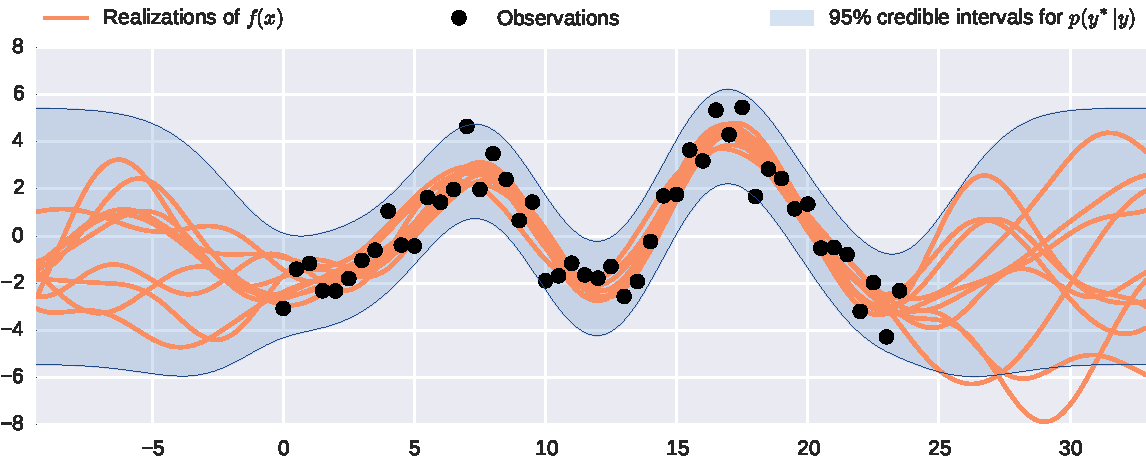
\includegraphics[width=1\textwidth]{../diagrams/PosteriorGP.pdf}}
    \end{overprint}
}

\frame{
    \frametitle{GP regression setting}
    So far we have assumed that the latent values, $\fV$, have been corrupted by Gaussian noise.
    Everything remains analytically tractable.
    \begin{align*}
        \text{Gaussian Prior:} & & \fV \sim \mathcal{GP}(\zerosVector, \Kff) = p(\fV)\\
        \text{Gaussian likelihood:} & & \yV \sim \gaussianSamp{\fV}{\noiseVar\eye} = \prod^{\numData}_{i=1} p(\yV_{i}|\fV_{i})\\
        \text{Gaussian posterior:} & & p(\fV|\yV) \propto \gaussianDist{\yV}{\fV}{\noiseVar\eye}\gaussianDist{\fV}{\zerosVector}{\Kff}
    \end{align*}
}

\section{Motivation}
\frame{
\frametitle{Outline}
    \tableofcontents[currentsection]
}

\frame{
    \frametitle{Motivation}
    \begin{itemize}
        \item You have been given some data you wish to model.
        \item You believe that the observations are connected through some underlying unknown function.
        \item You know from your understanding of the data generation process, that the observations are not Gaussian.
        \item You still want to learn, as best as possible, what is the unknown function being used, and make predictions.
    \end{itemize}
    \begin{overprint}
        \centerline{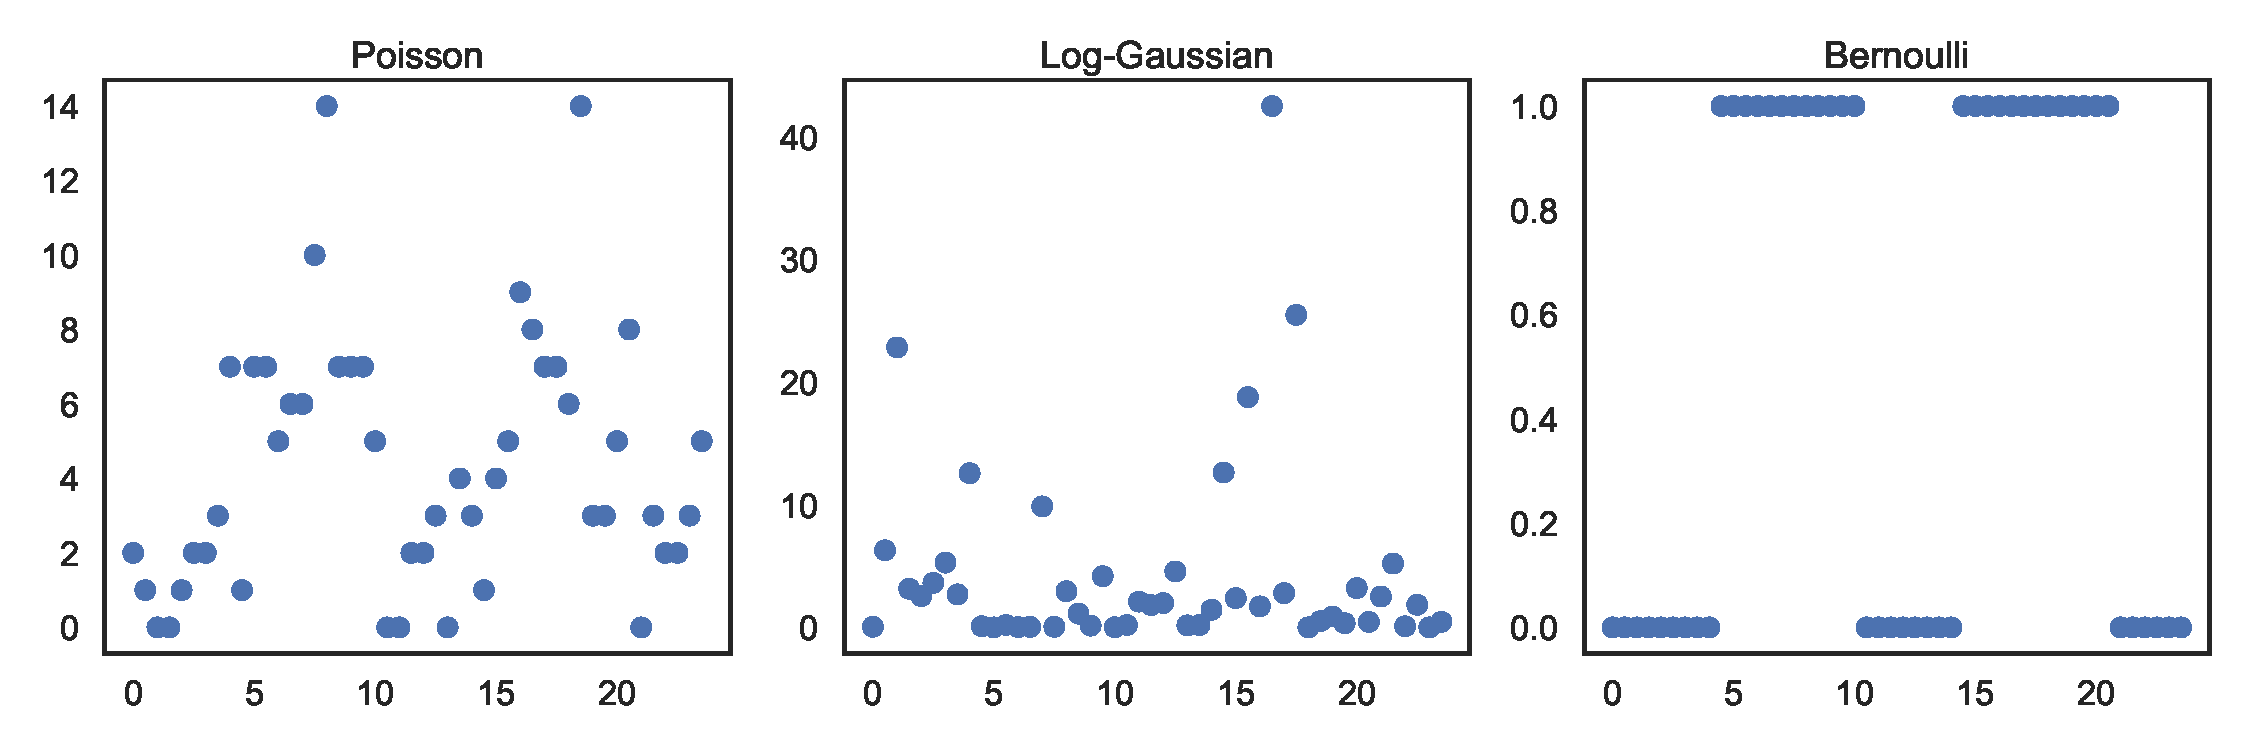
\includegraphics[width=.99\textwidth]{../diagrams/datatypes.pdf}}
    \end{overprint}
}

\frame{
    \frametitle{Likelihood}
    \begin{itemize}
        \uncover<+->{\item $p(\yV|\fV)$ is the probability that we would see some random variables, $\yV$, if we knew the latent function values $\fV$, which act as parameters.}
        \uncover<+->{\item Given the observed values for $\yV$ are fixed, it can also be seen as the likelihood that some latent function values, $\fV$, would give rise to the observed values of $\yV$. Note this is a \emph{function} of $\fV$, and doesn't integrate to $1$ in $\fV$.}
        \uncover<+->{\item Often observations aren't observed by simple Gaussian corruptions of the underlying latent function, $\fV$.}
        %\item So far assumed that the distortion of the underlying latent function, $\fV$, that gives rise to the observed data, $\yV$, is independent and normally distributed.
        \uncover<+->{\item In the case of count data, binary data, etc, we need to choose a different likelihood function.}
    \end{itemize}
}

\frame{
    \frametitle{Likelihood}
    \centering $p(y|f)$ as a function of y, with fixed f
    \begin{overprint}
        \centerline{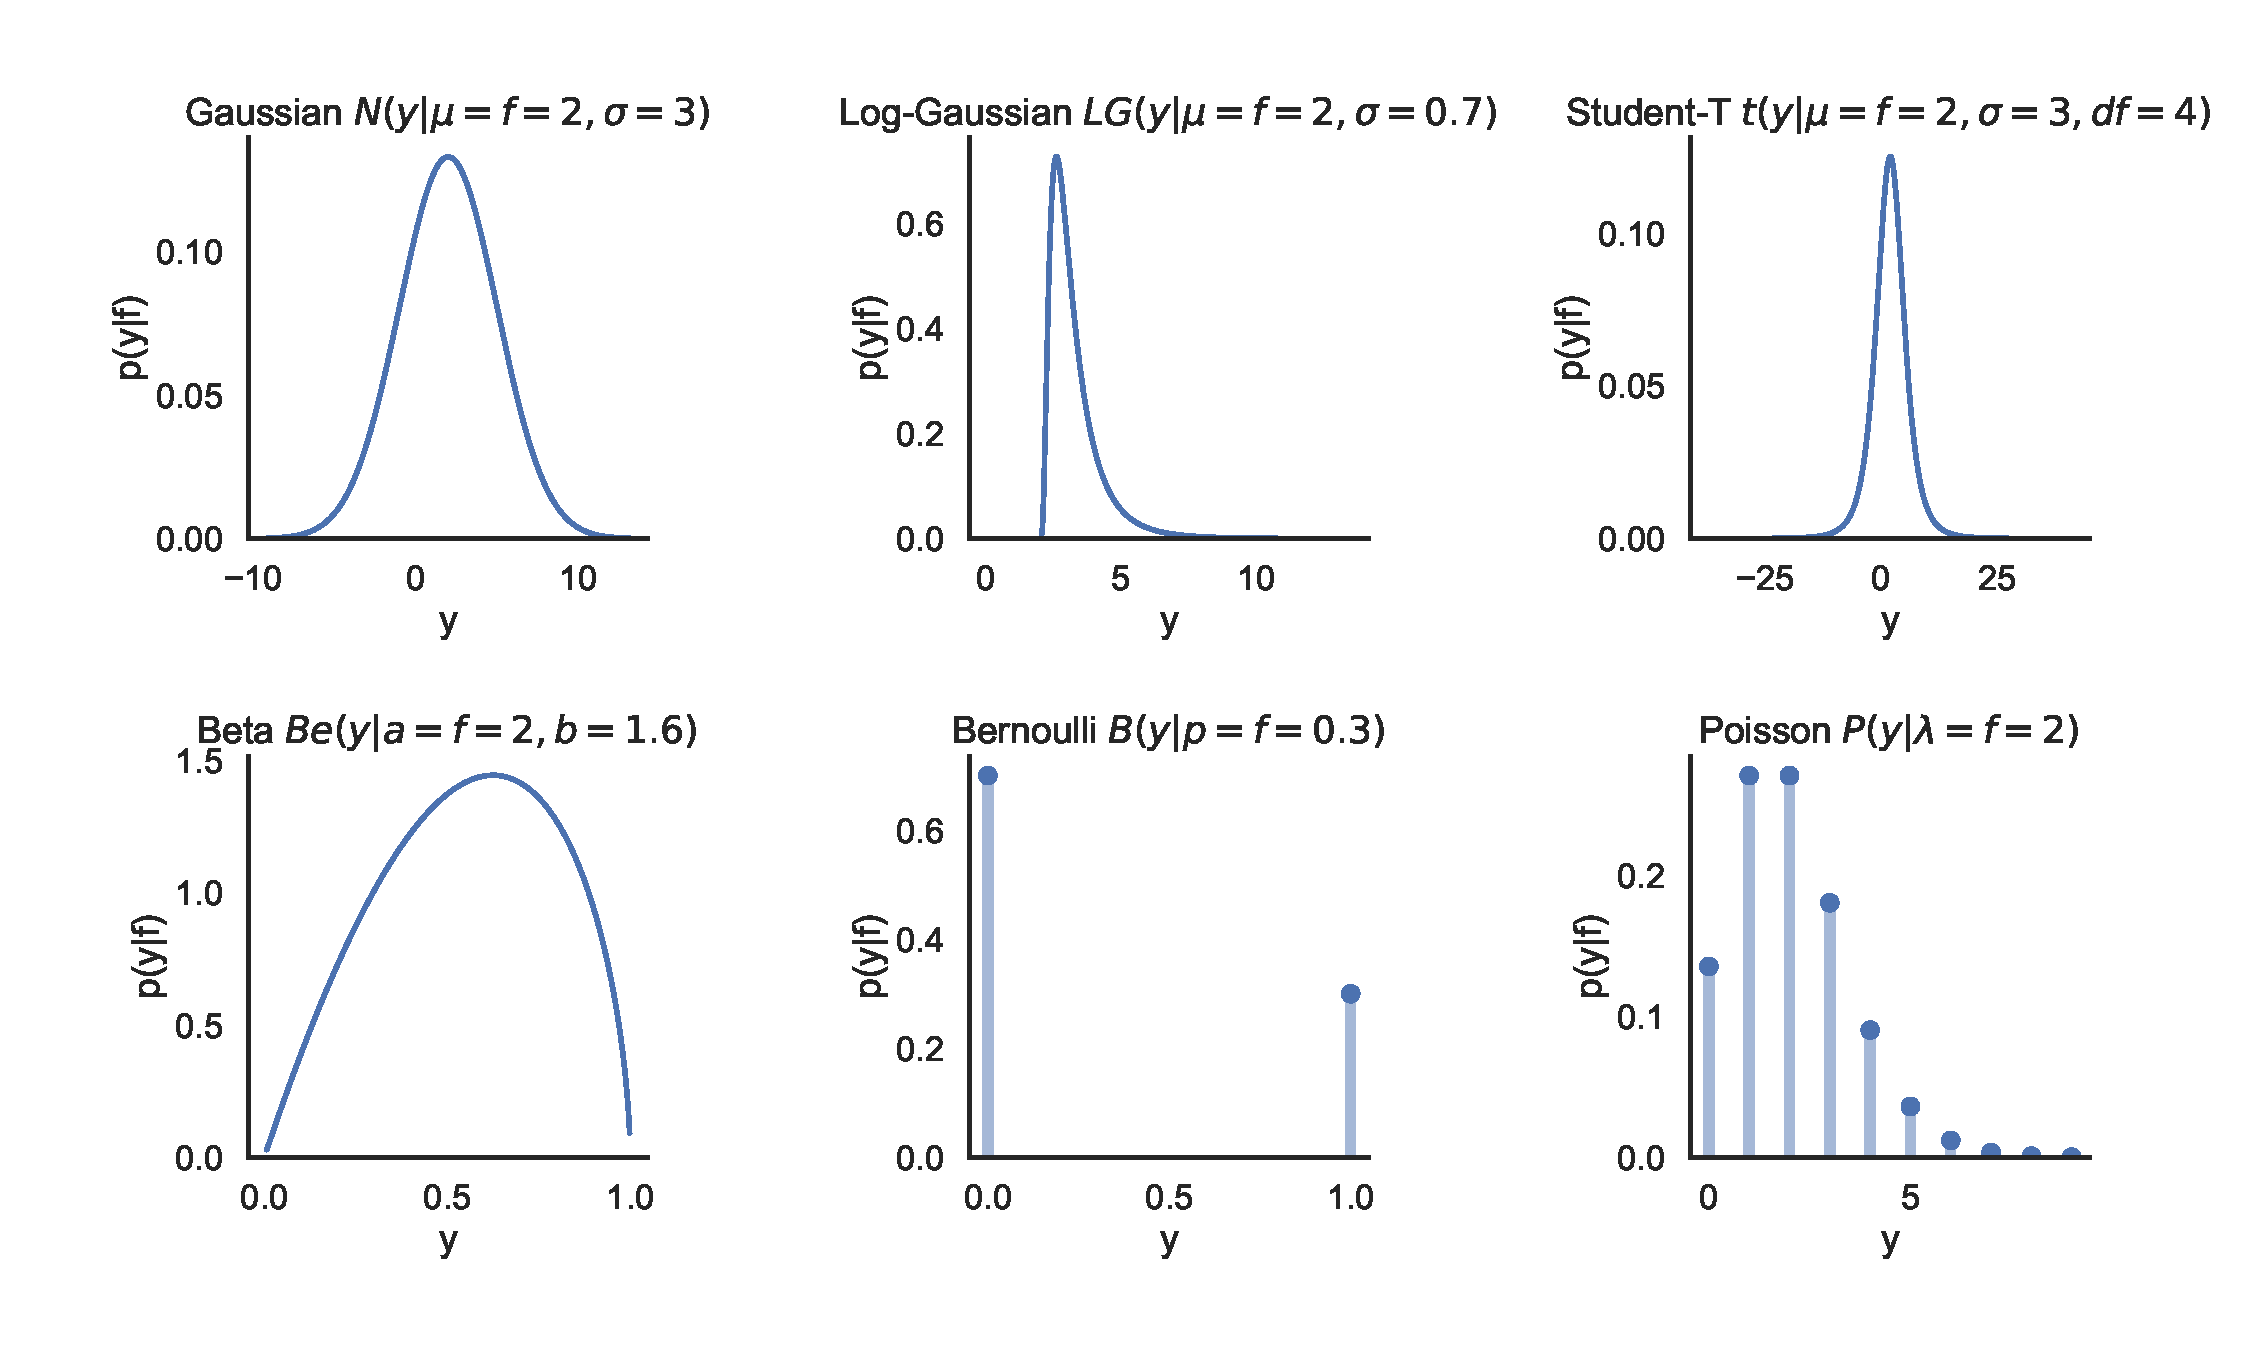
\includegraphics[width=.99\textwidth]{../diagrams/all_likelihoods.pdf}}
    \end{overprint}
}

\frame{
    \frametitle{Likelihood}
    \centering $p(y|f)$ as a function of f, with fixed y
    \begin{overprint}
        \centerline{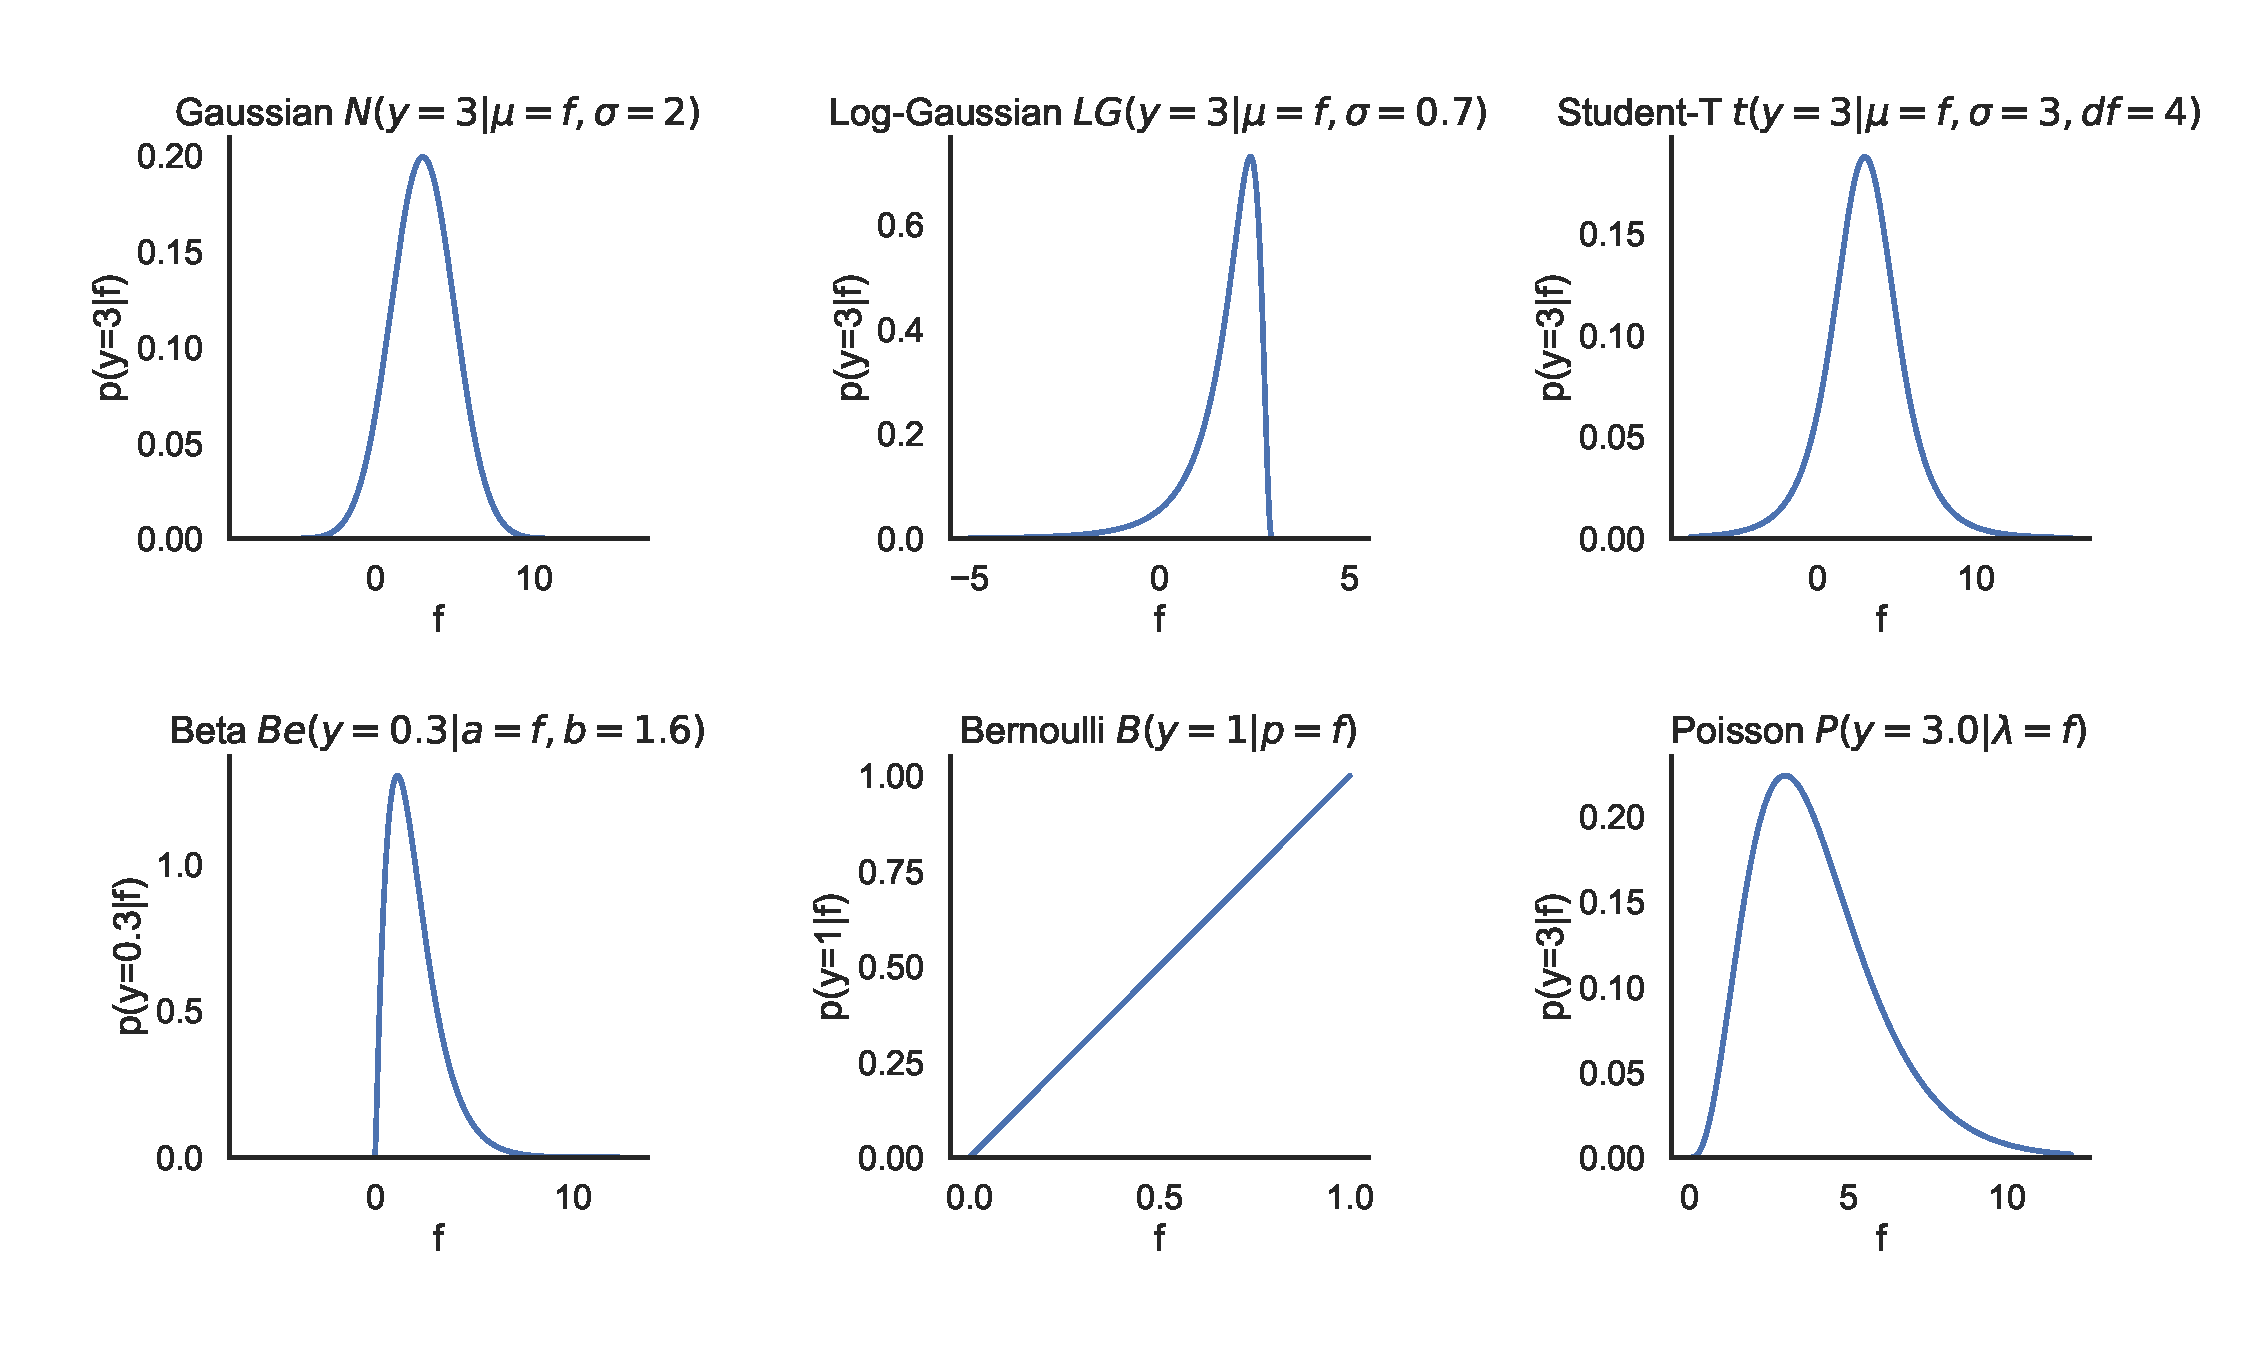
\includegraphics[width=.99\textwidth]{../diagrams/all_actual_likelihoods.pdf}}
    \end{overprint}
}
% ON THE BOARD ILLUSTRATE THE STUDENT-T

\frame{
    \frametitle{Binary example}
    \begin{itemize}
        \item Binary outcomes for $\yV_{i}$, $\yV_{i} \in [0,1]$.
        \item Model the probability of $\yV_{i} = 1$ with transformation of GP, with Bernoulli likelihood.
        \item Probability of $1$ must be between $0$ and $1$, thus use squashing transformation, $\lambda(\fV_{i}) = \Phi(\fV_{i})$.
    \end{itemize}
    \begin{align*}
        p(\yV_{i}|\lambda(\fV_{i})) = \left\{
            \begin{array}{ll}
                \lambda(\fV_{i}), & \text{if $\yV_{i} = 1$}\\
                1-\lambda(\fV_{i}), & \text{if $\yV_{i} = 0$}
            \end{array}
        \right.
    \end{align*}
    %\begin{align*}
        %p(\yV_{i}|\lambda(\fV_{i})) = \left\{
            %\begin{array}{ll}
                %1, & \text{with probability $\lambda(\fV_{i})$.}\\
                %0, & \text{with probability $1-\lambda(\fV_{i})$.}
            %\end{array}
        %\right.
    %\end{align*}
    %\begin{align*}
        %\yV_{i} = \left\{
            %\begin{array}{ll}
                %1, & \text{with probability $\lambda(\fV_{i})$.}\\
                %0, & \text{with probability $1-\lambda(\fV_{i})$.}
            %\end{array}
        %\right.
    %\end{align*}
    \centerline{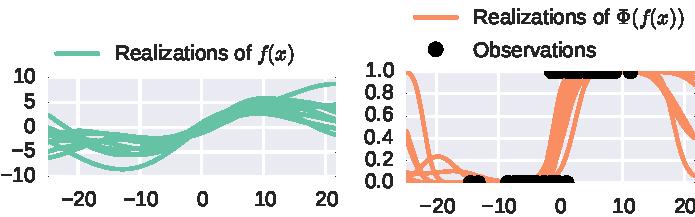
\includegraphics[width=1.0\textwidth]{../diagrams/BernoulliPosterior.pdf}}
}

\frame{
    \frametitle{Count data example}
    \begin{overprint}
    \begin{itemize}
        \item Non-negative and discrete values only for $\yV_{i}$, $\yV_{i} \in \mathbb{N}$.
        \item Model the \emph{rate} or \emph{intensity}, $\lambda$, of events with a transformation of a Gaussian process.
        \item Rate parameter must remain positive, use transformation to maintain positiveness $\lambda(\fV_{i}) = \exp(\fV_{i})$ or $\lambda(\fV_{i}) = \fV_{i}^2$
    \end{itemize}
    \begin{align*}
        \yV_{i} \sim \text{Poisson}(\yV_{i}|\lambda_{i} = \lambda(\fV_{i}))\quad\quad
        \text{Poisson}(\yV_{i}|\lambda_{i}) = \frac{\lambda_{i}^{\yV_{i}}}{!\yV_{i}}e^{-\lambda_{i}}
    \end{align*}
\end{overprint}
\begin{overprint}
    \centerline{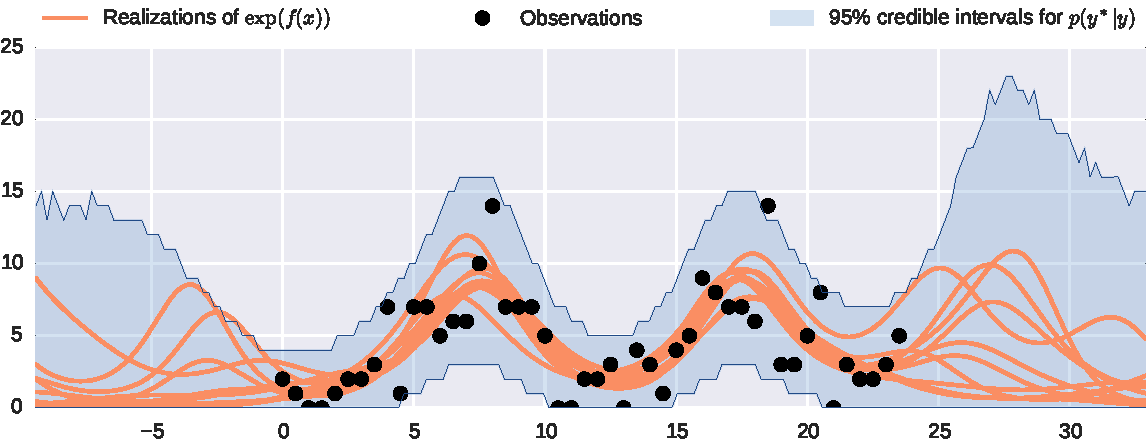
\includegraphics[width=.8\textwidth]{../diagrams/PoissonPosterior.pdf}}
\end{overprint}
}

\frame{
    \frametitle{Application example}
\begin{columns}[onlytextwidth]
    \begin{column}{0.5\textwidth}
        \begin{itemize}
            \item Chicago crime counts.
            \item Same Poisson likelihood.
            \item 2D-input to kernel.
        \end{itemize}
    \end{column}
    \begin{column}{0.5\textwidth}
        \begin{overprint}
            \centerline{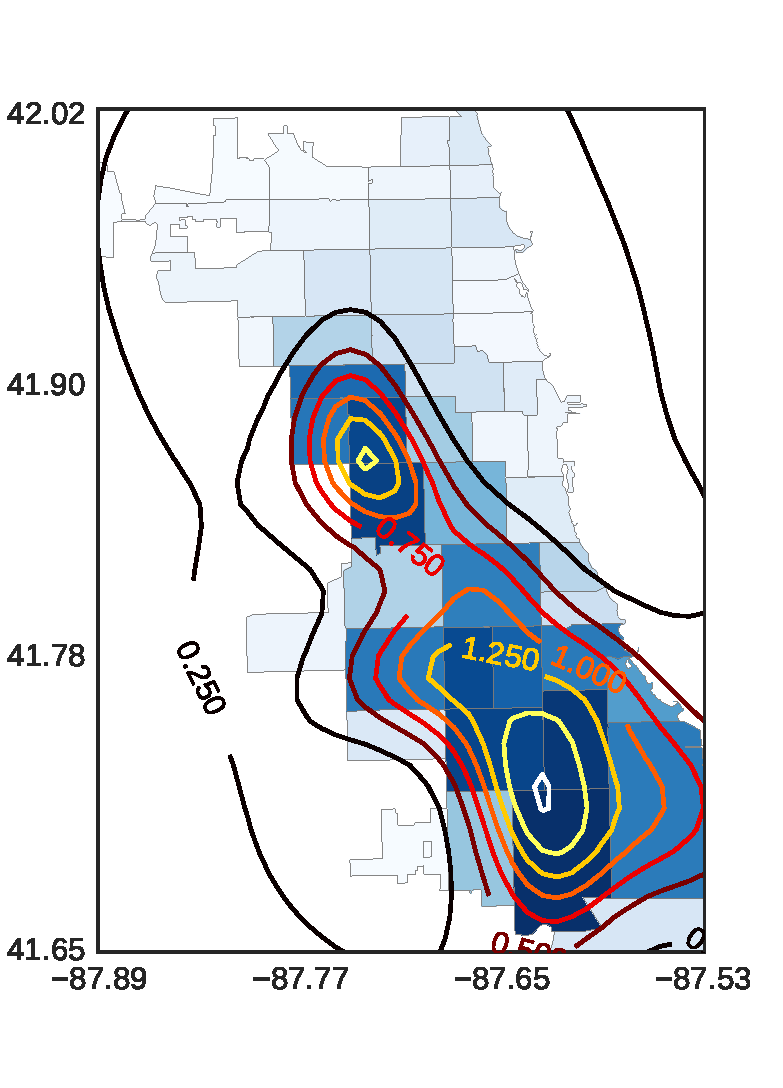
\includegraphics[width=\textwidth]{../diagrams/crime_func_f_fast.pdf}}
        \end{overprint}
    \end{column}
\end{columns}
}

%\frame{
    %\frametitle{Application example}
    %MORE COMPLEX MOTIVATING APPLICATION. MNIST MULTICLASS
%}


\section{Non-Gaussian posteriors}
\frame{
\frametitle{Outline}
    \tableofcontents[currentsection]
}

\frame{
    \frametitle{Non-Gaussian posteriors}
    \begin{itemize}
        \item Exact computation of posterior is no longer analytically tractable due to non-conjugate Gaussian process prior to non-Gaussian likelihood, $p(\yV|\fV)$.
    \end{itemize}
    \begin{equation*}
        {\color{intract}p(\fV|\yV)} = \frac{p(\fV)\prod^{\numData}_{i=1}p(\yV_{i}|\fV_{i})}{\color{intract}\int p(\fV)\prod^{\numData}_{i=1}p(\yV_{i}|\fV_{i})\,d\fV}
    \end{equation*}

    Why is it so difficult?
}

\frame{
    \frametitle{Non-Gaussian posteriors illustrated}
    \begin{itemize}
        \item Consider one observation, $y_{1} = 1$, at input $x_{1}$.
        \item Can normalise easily with numerical integration, $\int p(y_1=1|\lambda(f_1))p(f_1) df_1$.
    \end{itemize}
    \begin{overprint}
        \onslide<1>\centerline{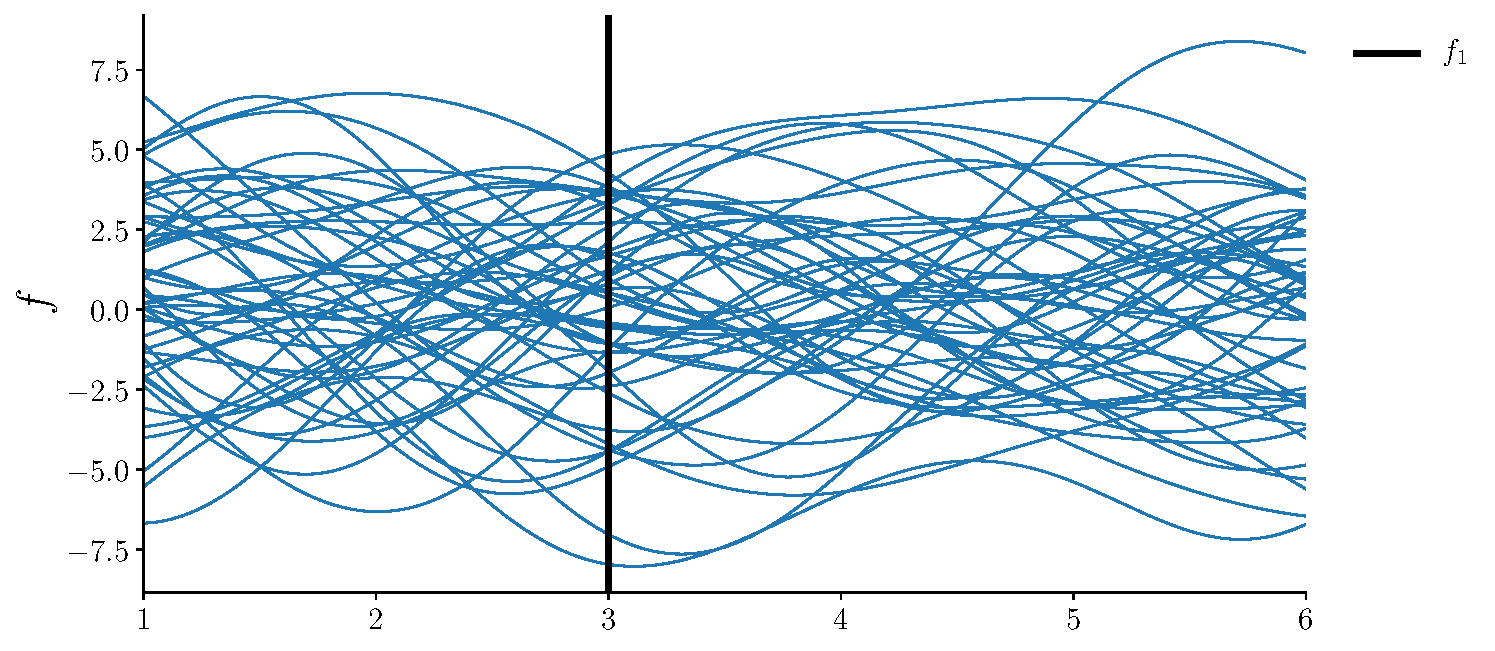
\includegraphics[width=0.9\textwidth]{../diagrams/1d_gp_prior_samples.pdf}}
        \onslide<2>\centerline{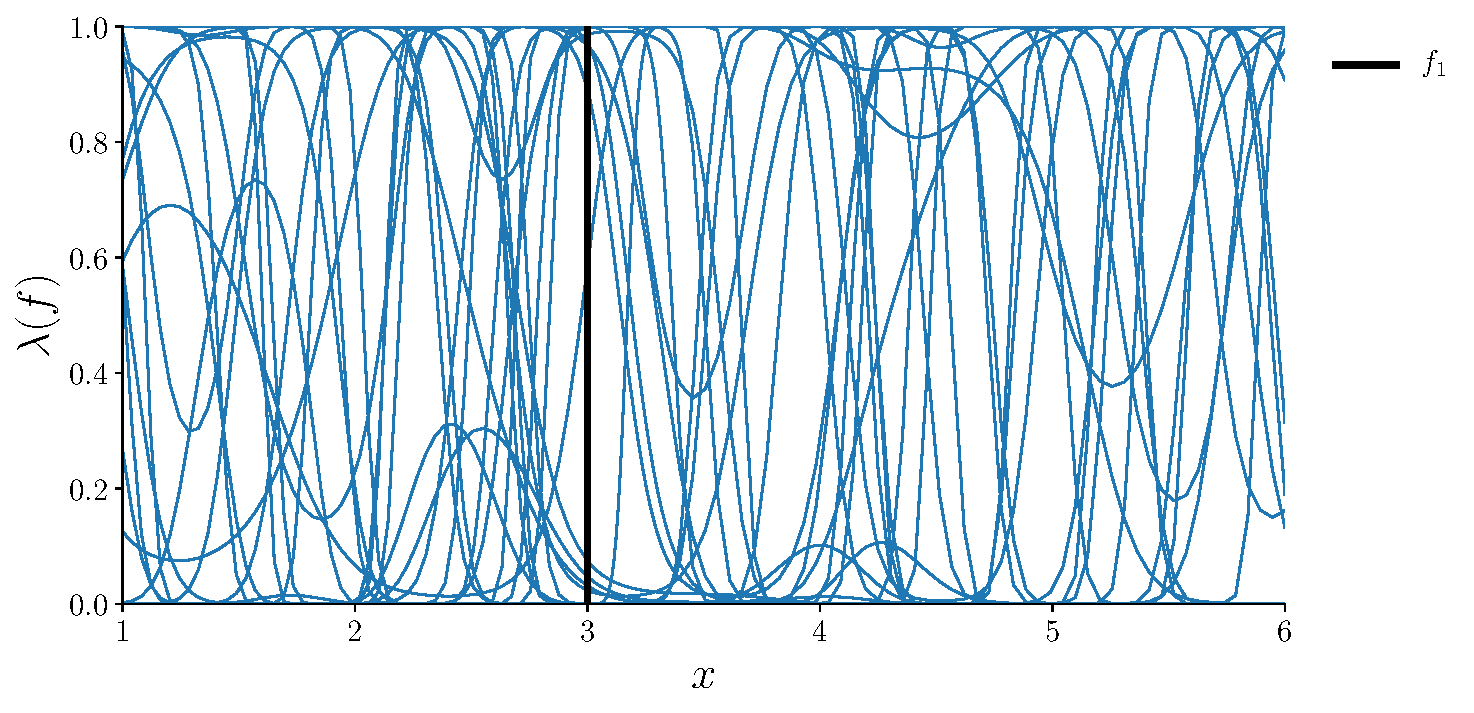
\includegraphics[width=0.9\textwidth]{../diagrams/1d_squashed_gp_prior_samples.pdf}}
        \onslide<3>\centerline{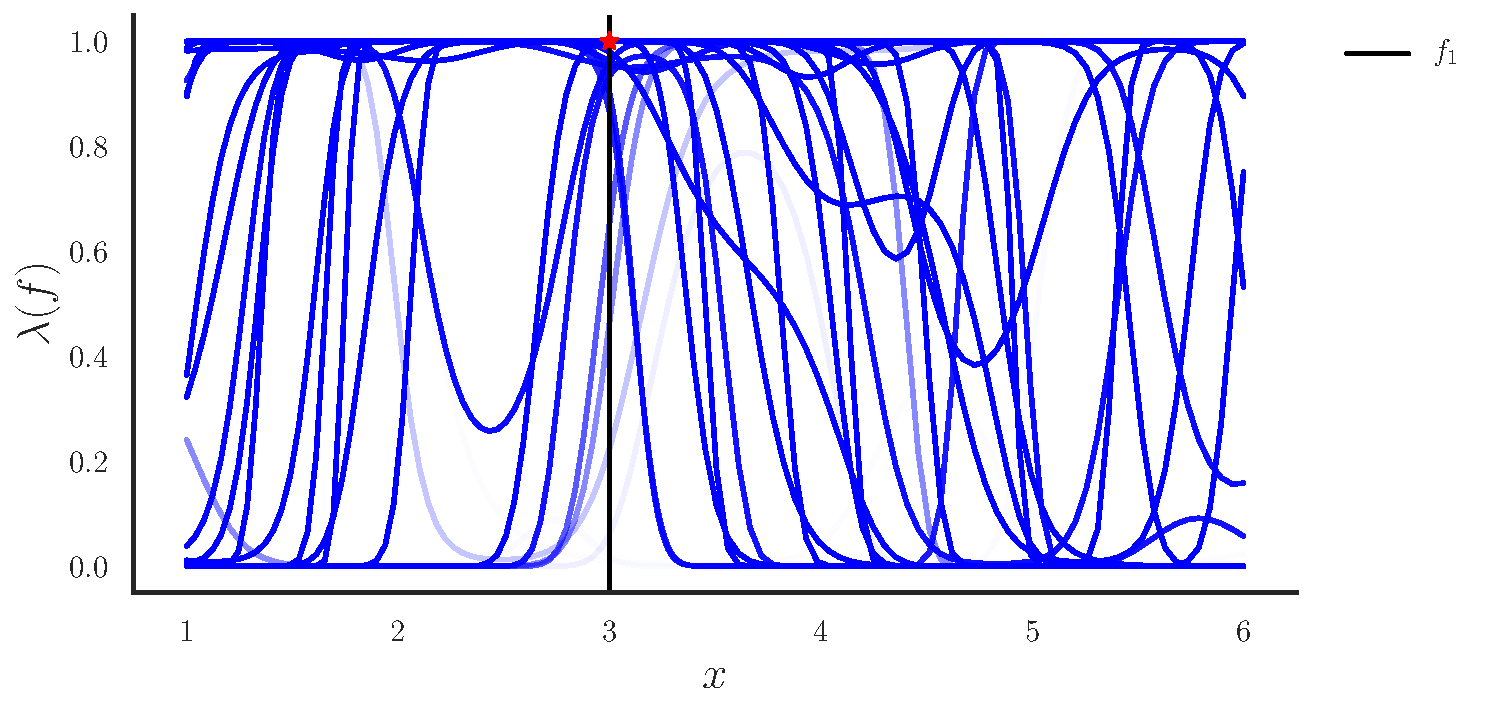
\includegraphics[width=0.9\textwidth]{../diagrams/1d_gp_post_samples.pdf}}
    \end{overprint}
}
% So I've told you that its difficult to do this integration, but I now want to illustrate why this is the case. Often when people talk about the posterior they only really illustrate the posterior in one dimension, I think its useful to understand what is really happening when we get to this problem with Gaussian processes, that is we need to do this integral in a far higher dimension.

\frame{
    \frametitle{Non-Gaussian posteriors illustrated}
    \begin{overprint}
        \centerline{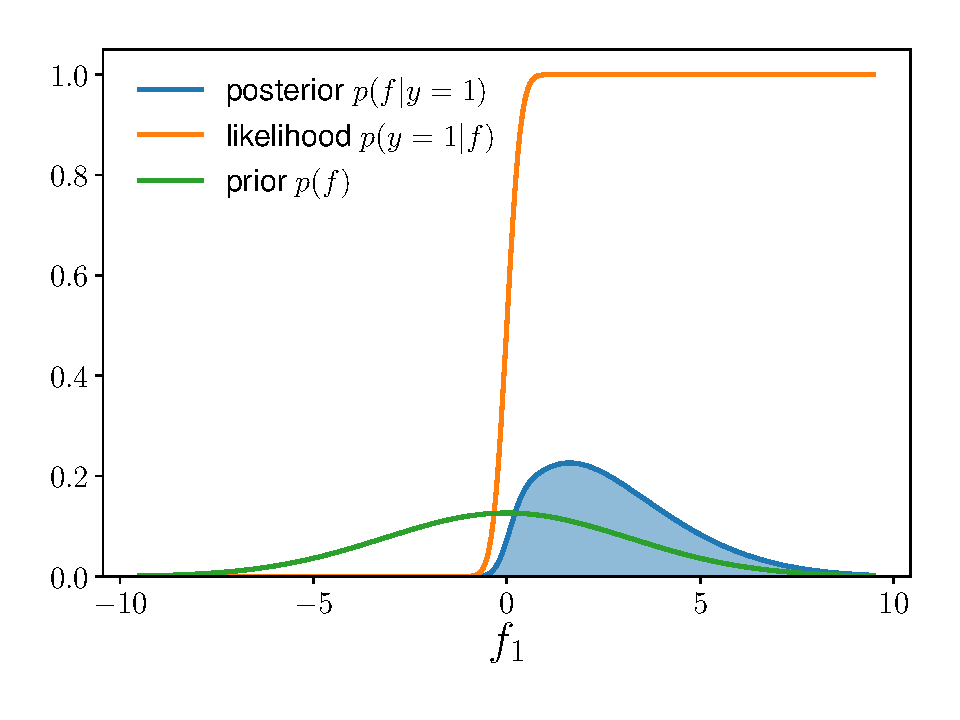
\includegraphics[width=0.9\textwidth]{../diagrams/1d_marginals.pdf}}
    \end{overprint}
}

\frame{
    \frametitle{Non-Gaussian posteriors illustrated}
    \begin{itemize}
        \item Now two observations, $y_{1} = 1$ and $y_{2} = 1$ at $x_{1}$ and $x_{2}$
        \item Need to calculate the joint posterior, $p(\fV|\yV) = p(f_{1}, f_{2}| y_{1}=1, y_{2}=1)$.
        \item Requires 2D integral $p(y_1=1,y_2=1|\lambda(f_1),\lambda(f_2))p(f_1, f_2) df_1 df_2$.
    \end{itemize}
    \begin{overprint}
        \onslide<1>\centerline{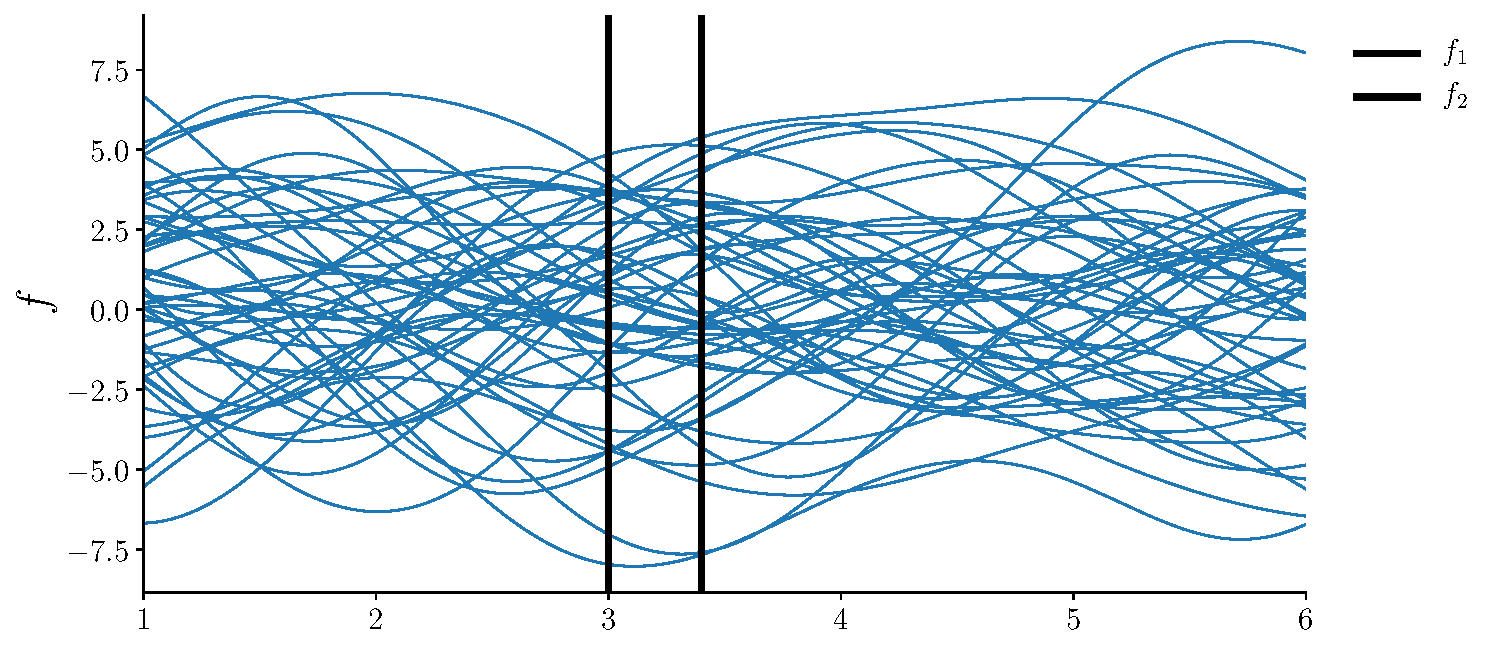
\includegraphics[width=0.8\textwidth]{../diagrams/2d_gp_prior_samples.pdf}}
        \onslide<2>\centerline{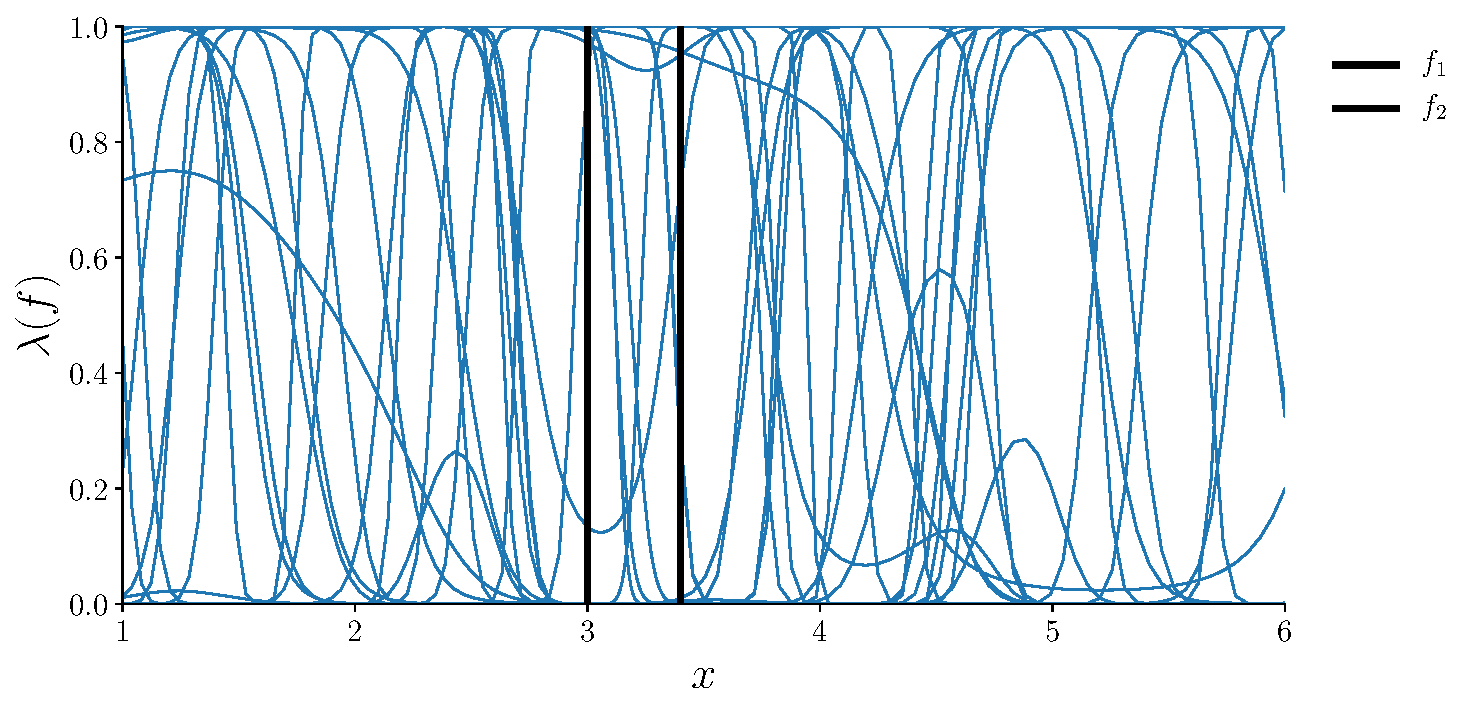
\includegraphics[width=0.8\textwidth]{../diagrams/2d_squashed_gp_prior_samples.pdf}}
        \onslide<3>\centerline{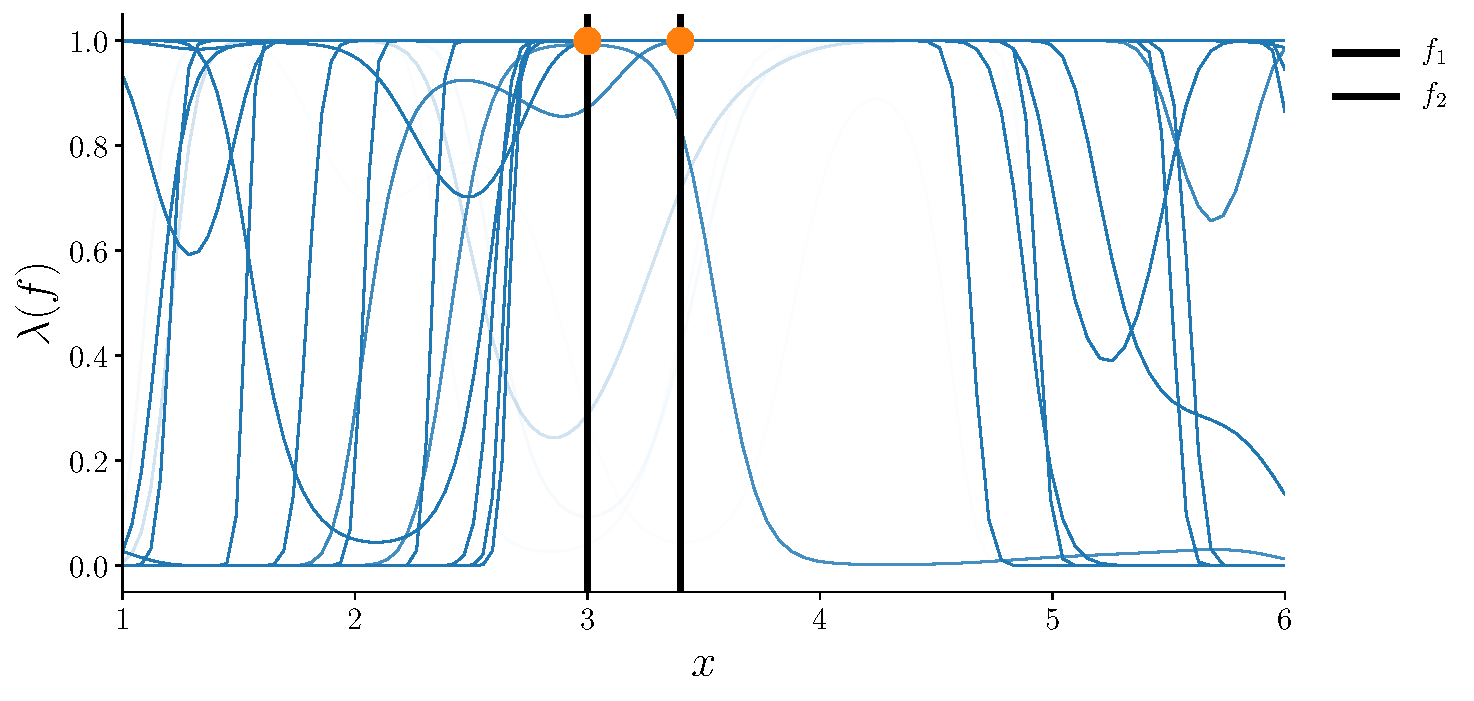
\includegraphics[width=0.8\textwidth]{../diagrams/2d_gp_post_samples.pdf}}
    \end{overprint}
}

\frame{
    \frametitle{Non-Gaussian posteriors illustrated}
    \begin{itemize}
        \item To find the true posterior values, we need to perform a two dimensional integral.
        \item Still possible, but things are getting more difficult quickly.
    \end{itemize}
    \begin{overprint}
        \onslide<1>\centerline{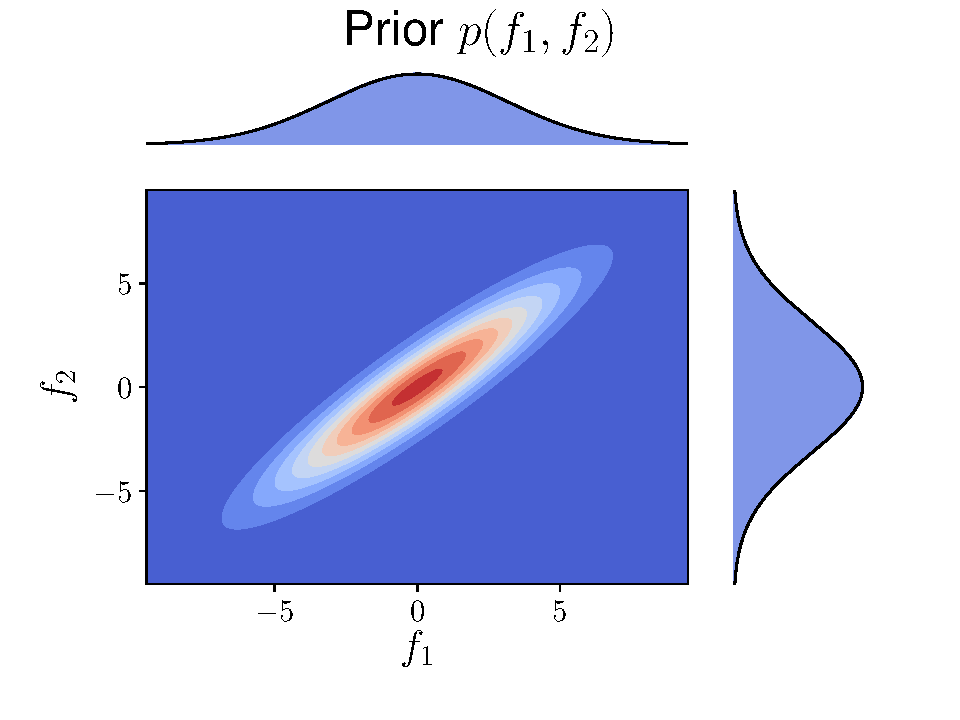
\includegraphics[width=0.8\textwidth]{../diagrams/2d_joint_prior.pdf}}
        \onslide<2>\centerline{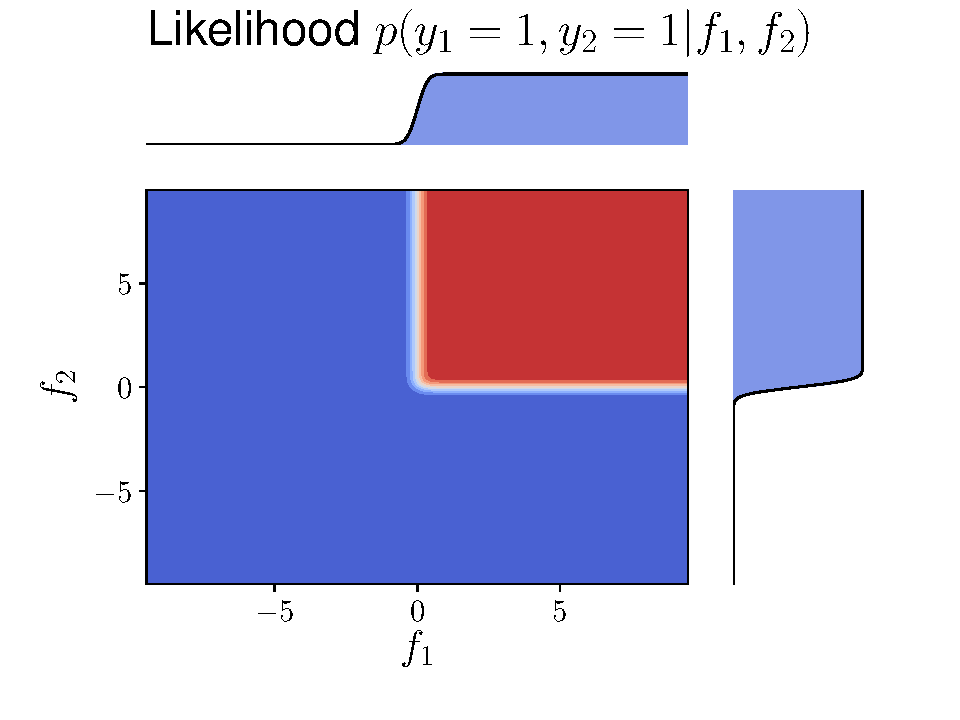
\includegraphics[width=0.8\textwidth]{../diagrams/2d_joint_likelihood.pdf}}
        \onslide<3>\centerline{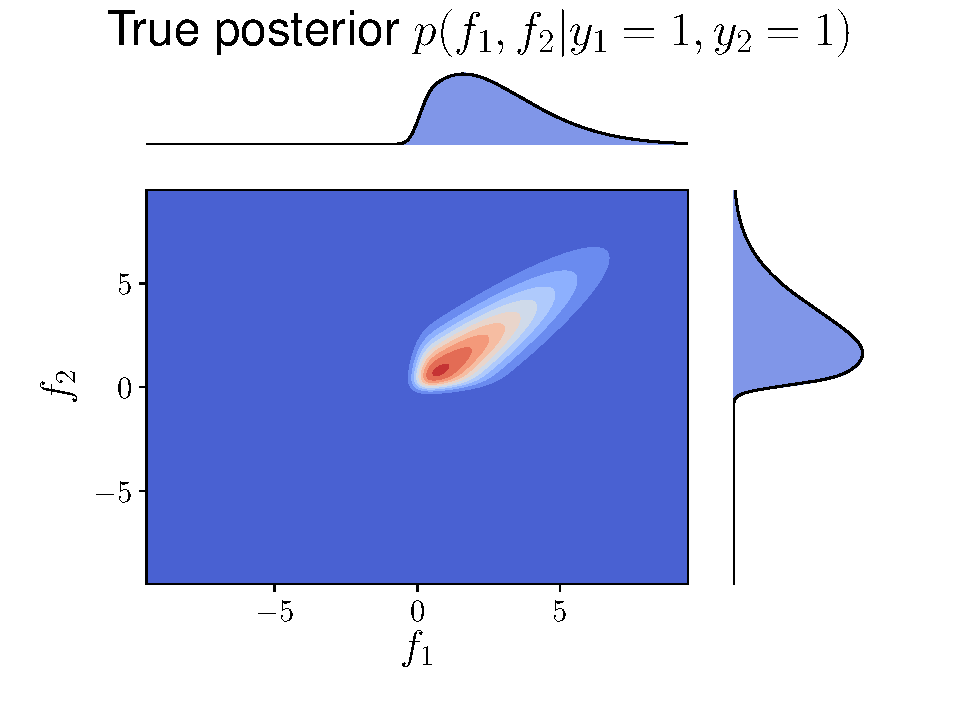
\includegraphics[width=0.8\textwidth]{../diagrams/2d_joint_posterior.pdf}}
    \end{overprint}
}

\frame{
   \frametitle{Approaches to handling non-Gaussian posteriors}
   Generally fall into two areas:
   \begin{itemize}
        \item Sampling methods that obtain samples of the posterior.
        \item Approximation of the posterior with something of known form.
   \end{itemize}

   Today we will focus on the latter.\\~\\

    \centerline{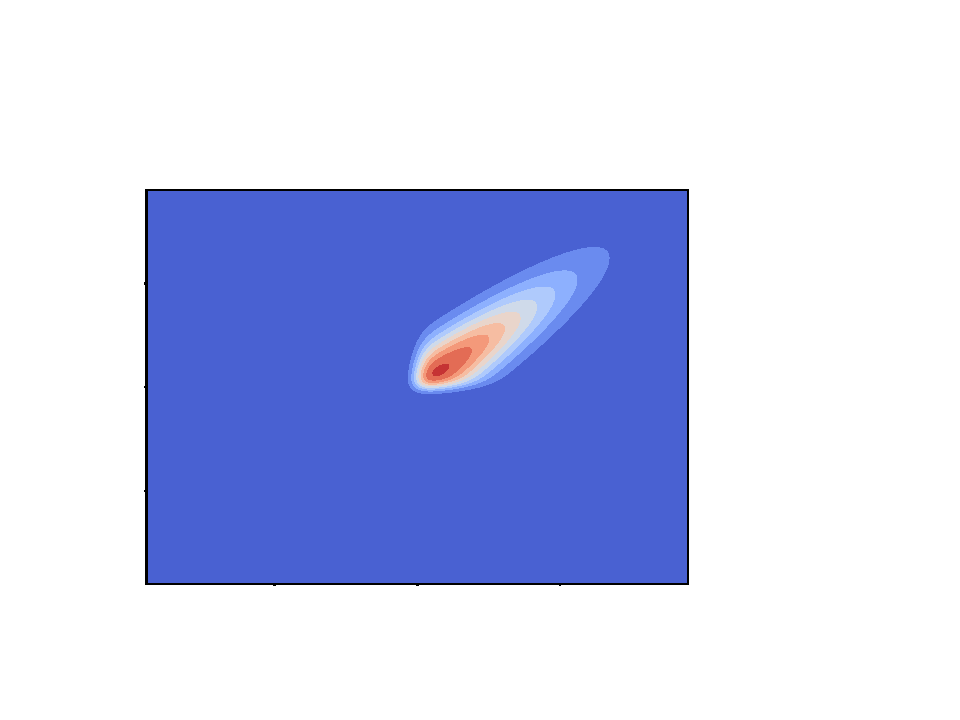
\includegraphics[width=0.3\textwidth]{../diagrams/2d_joint_posterior_no_marginals.pdf}
                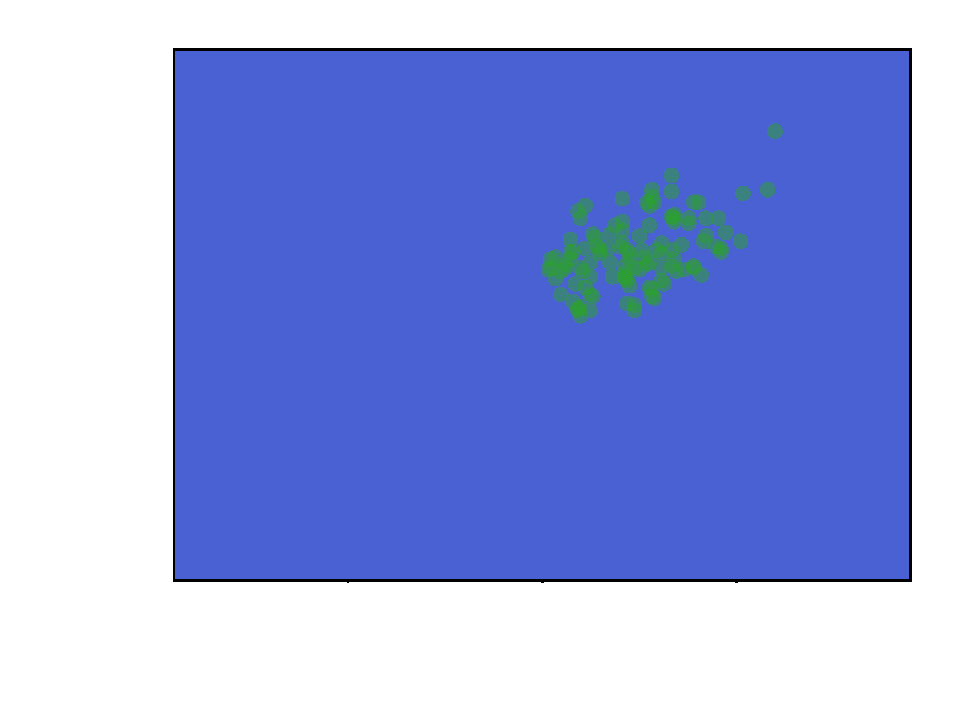
\includegraphics[width=0.3\textwidth]{../diagrams/2d_joint_posterior_samples.pdf}
                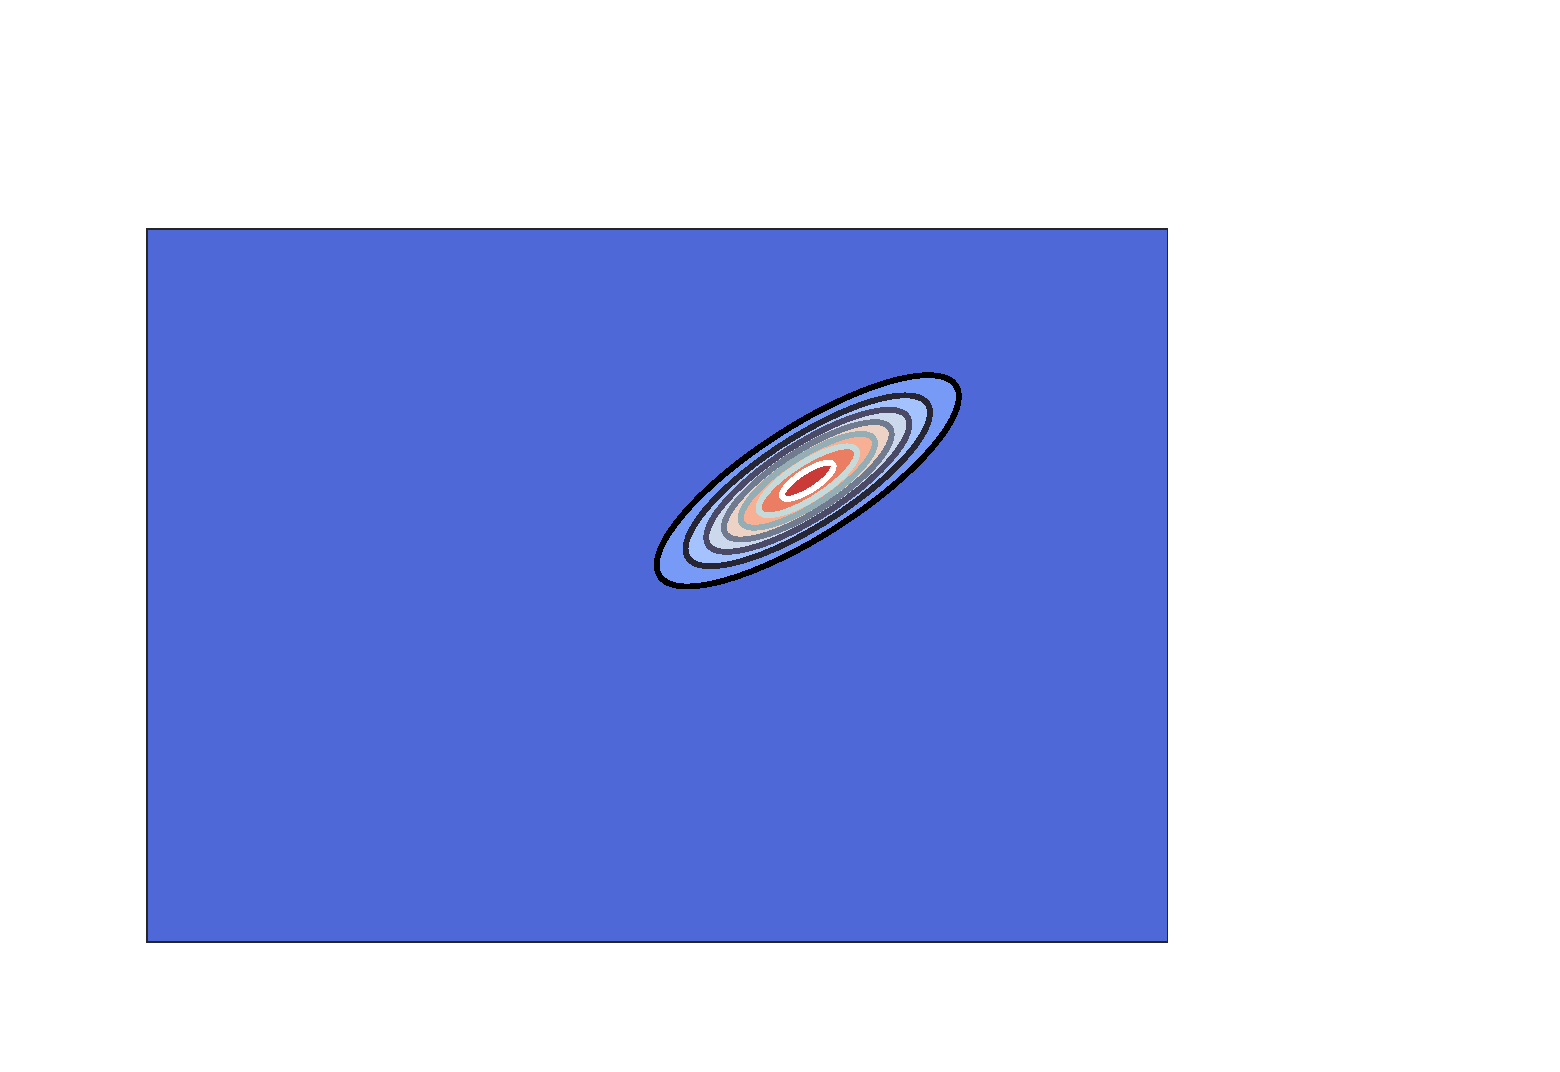
\includegraphics[width=0.31\textwidth]{../diagrams/joint_kl_no_marginals.pdf}}
}

\frame{
    \frametitle{Non-Gaussian posterior approximation}
    \begin{itemize}
        \item Various methods to make a Gaussian approximation, ${\color{intract}p(\fV|\yV)} \approx q(\fV) = \gaussianDist{\fV}{\mathbf{\mu}=?}{\Cmat=?}$.
        \item Only need to obtain an approximate posterior at the training locations.
        \item At test locations, the data only effects their probabily via the posterior at these locations.
    \end{itemize}
    \begin{align*}
        p(\fV, \fV^{*}|\xV^{*}, \xV, \yV) &= p(\fV^*|\fV, \xV^{*})p(\fV|\xV, \yV)\\
        &\propto p(\fV^{*}|\fV, \xV^{*})p(\yV|\fV, \xV)p(\fV|\xV)
    \end{align*}
}

\frame{
    \frametitle{Why do we want an the posterior anyway?}
    True posterior, posterior approximation, or samples are needed to make predictions at new locations, $\xV^{*}$.
    \begin{align*}
        p(\fV^{*}|\xV^{*}, \xV, \yV) &= \int p(\fV^{*}|\fV, \xV^{*}){\color{intract}{p(\fV|\yV, \xV)}} d\fV\\
        q(\fV^{*}|\xV^{*}, \xV, \yV) &= \int p(\fV^{*}|\fV, \xV^{*})q(\fV|\xV) d\fV
    \end{align*}
}

\section{Approximate methods}
\frame{
\frametitle{Outline}
    \tableofcontents[currentsection]
}

\frame{
    \frametitle{Methods overview}
    Given choice of Gaussian approximation of posterior. How do we choose the parameter values $\mu$ and $\Cmat$?

    There a number of different methods in which to choose how to set the parameters of our Gaussian approximation.
}

\frame{
    \frametitle{Parameters effect - mean}
    %\animategraphics[loop,width=1\linewidth]{20}{../diagrams/animations/mean-change-frame-}{0}{199}
}

\frame{
    \frametitle{Parameters effect - variance}
    %\animategraphics[loop,width=1\linewidth]{20}{../diagrams/animations/L-change-frame-}{0}{199}
}

\frame{
    \frametitle{How to choose the parameters?}
    Two approaches that we might take:
    \begin{itemize}
        \item Is to match the mean and variance at some point, for example the mode.
        \item Attempt to minimise some divergence measure between the approximate distribution and the true distribution.
    \end{itemize}

    \begin{itemize}
        \item Laplace takes the former
        \item Variational bayes takes the latter
        \item EP kind of takes the latter
    \end{itemize}
}

\subsection{Laplace approximation}
\frame{
\frametitle{Outline}
    \tableofcontents[currentsection]
}

\frame{
    \frametitle{Laplace approximation}
    Task: for some generic random variable, $z$, and data, $y$, find a good approximation to difficult to compute posterior distribution, $\color{intract}p(z|y)$.\\~\\
    Laplace approach: fit a Gaussian by matching the curvature at the modal point of the posterior.
    \begin{itemize}
        \item Use a second-order taylor expansion around the mode of the log-posterior.
        \item Use the expansion to find an equivalent Gaussian in the probability space.
    \end{itemize}
}

\frame{
    \frametitle{Laplace approximation}
    \begin{itemize}
        \item Log of a Gaussian distribution, $q(\fV) = \gaussianDist{\fV}{\hat{\mu}}{\hat{\Cmat}}$, is a quadratic function of $\fV$.
        \item A second-order taylor expansion is an approximation of a function using only quadratic terms.
        \item Laplace approximation expands the un-normalised posterior, and then uses it to set the linear and quadratic terms of the log $q(\fV)$.
        \item The first and second derivatives of the form of the log-posterior, at the mode, will match the derivatives of the approximate Gaussian at this same point.
    \end{itemize}
}

\frame{
    \frametitle{Second-order taylor expansion}
    \begin{align*}
        \uncover<+->{p(\fV|\yV) &= \frac{1}{{\color{intract}Z}}h(\fV)\\}
        \uncover<+->{\log p(\fV|\yV) &= \log \frac{1}{{\color{intract}Z}} + \log h(\fV)\\}
        \uncover<+->{&\approx \log \frac{1}{{\color{intract}Z}} + \log h(\aV) + \frac{d\log h(\aV)}{d\aV}(\fV - \aV)\\
        &+ \frac{1}{2}(\fV - \aV)^\top\frac{d^{2}\log h(\aV)}{d\aV^{2}}(\fV - \aV)}
    \end{align*}
    \uncover<+->{
    In our case we want to make our expansion around the mode, $\hat{\fV}$:
    \begin{align*}
        \left.\frac{d\log h(\aV)}{d\aV}\right|_{\aV=\hat{\fV}} = \zerosVector
    \end{align*}
}
}

\frame{%
    \frametitle{Second-order taylor expansion}
    \begin{align*}
        \uncover<+->{\log p(\fV|\yV) &\approx \log \frac{1}{{\color{intract}Z}} + \log h(\hat{\fV}) + \frac{d\log h(\hat{\fV})}{d\hat{\fV}}(\fV - \hat{\fV})\\
        &+ \frac{1}{2}(\fV - \hat{\fV})^\top\frac{d^{2}\log h(\hat{\fV})}{d\hat{\fV}^{2}}(\fV - \hat{\fV})\\}
        \uncover<+->{p(\fV|\yV) &= \frac{1}{{\color{intract}Z}}h(\hat{\fV})\exp\left\{-\frac{1}{2}(\fV - \hat{\fV})^{\top}\left(-\frac{d^{2}\log h(\hat{\fV})}{d\fV^{2}}\right)(\fV - \hat{\fV})\right\}\\}
        \uncover<+->{&= \gaussianDist{\fV}{\hat{\fV}}{\left(-\frac{d^{2}\log h(\hat{\fV})}{d\fV^{2}}\right)^{-1}}}
    \end{align*}
}

\frame{%
    \frametitle{Laplace appoximation for Gaussian processes}
    In our case, $h(\fV) = p(\yV|\fV)p(\fV)$, so we need to evaluate
    \begin{align*}
        -\frac{d^{2}\log h(\hat{\fV})}{d\fV^{2}} &= -\frac{d^{2}(\log p(\yV|\hat{\fV}) + \log p(\hat{\fV}))}{d\fV^{2}}\\
        &= -\frac{d^{2}\log p(\yV|\hat{\fV})}{d\fV^{2}} + \mathbf{K}^{-1}\\
        &\triangleq \Wmat + \mathbf{K}^{-1}
    \end{align*}
    giving a posterior approximation:
    \begin{align*}
        p(\fV|\yV) \approx q(\fV) = \gaussianDist{\fV}{\hat{\fV}}{\left(\Wmat + \mathbf{K}^{-1}\right)^{-1}}
    \end{align*}
    }

\frame{
    \frametitle{Laplace approximation - algorithm overview}
    \begin{itemize}
        \item Find the mode, $\hat{\fV}$ of the true log posterior, via Newton's method.
        \item Use second-order Taylor expansion around this modal value.
        \item Form Gaussian approximation setting the mean equal to the posterior mode, $\hat{\fV}$, and matching the curvature.
        \item ${\color{intract}p(\fV|\yV)} \approx q(\fV|\muV,\Cmat) = \gaussianDist{\fV}{\hat{\fV}}{(\mathbf{K}^{-1} + \Wmat)^{-1}}$
        \item $\Wmat \triangleq -\frac{d^{2}\log p(\yV|\hat{\fV})}{d\hat{\fV}^{2}}$.
        \item For factorizing likelihoods (most), $\Wmat$ is diagonal.
    \end{itemize}
}
\note{The actual optimization is in log space, but here we show the result in the distribution space}

\frame{
    \frametitle{Visualization of Laplace}
    %\animategraphics[controls]{1}{../diagrams/laplace-anim}{0}{6}
    \centering
    \multiinclude[<+>][format=pdf,graphics={scale=0.6}]{../diagrams/animations/laplace-anim-log-Poisson}
}
\frame{
    \frametitle{Visualization of Laplace}
    %\animategraphics[controls]{1}{../diagrams/laplace-anim}{0}{6}
    \centering
    \multiinclude[<+>][format=pdf,graphics={scale=0.6}]{../diagrams/animations/laplace-anim-full-Poisson}
}

\frame{
    \frametitle{Visualise of Laplace - Bernoulli}
    \centering
    \multiinclude[<+>][format=pdf,graphics={scale=0.6}]{../diagrams/animations/laplace-anim-full-Bernoulli}
}

\subsection{Variational bayes}
\frame{
\frametitle{Outline}
    \tableofcontents[currentsection]
}

\frame{
    \frametitle{Variational Bayes (VB)}
    Task: for some generic random variable, $z$, and data, $y$, find a good approximation to difficult to compute posterior distribution, $\color{intract}p(z|y)$.\\~\\
    VB approach: minimise a divergence measure between an approximate posterior, $\color{tract}q(z)$ and true posterior, $\color{intract}p(z|y)$.
    \begin{itemize}
        \item KL divergence, $\color{intract}\KL{q(z)}{p(z|y)}$.
        \item Minimize this with respect to parameters of $\color{tract}q(z)$.
    \end{itemize}
}
% previously tried to approximate the posterior using a local point. Really want something that more globally captures the characteristics of the non-Gaussian posterior
% why KL? What about others? Alpha, F?

\frame{
    \frametitle{KL divergence}
    \begin{itemize}
        \item General for any two distributions $q(\xV)$ and $p(\xV)$.
        \item $\KL{q(\xV)}{p(\xV)}$ is the average additional amount of information required to specify the values of $\xV$ as a result of using an approximate distribution $q(\xV)$ instead of the true distribution, $p(\xV)$.
        \item $\KL{q(\xV)}{p(\xV)} = \expectationDist{\log \frac{q(\xV)}{p(\xV)}}{q(\xV)}$
        \item Always 0 or positive, not symmetric.
        \item Lets look at how it changes with response to changes in the approximating distribution.
    \end{itemize}
}

\frame{
    \frametitle{KL varying mean}
    %\animategraphics[controls]{1}{../diagrams/KL_gaussian_mu}{0}{6}
    %\animategraphics[loop,width=1\linewidth]{12}{../diagrams/KL_gaussian_mu-}{0}{4}
    \multiinclude[<+>][format=pdf,graphics={scale=0.4}]{../diagrams/KL_gaussian_mu}
}

\frame{
    \frametitle{KL varying variance}
    %\animategraphics[controls]{1}{../diagrams/KL_gaussian_mu}{0}{6}
    %\animategraphics[loop,width=1\linewidth]{12}{../diagrams/KL_gaussian_var-}{0}{4}
    \multiinclude[<+>][format=pdf,graphics={scale=0.4}]{../diagrams/KL_gaussian_var}
}

\frame{
    \frametitle{Variational Bayes}
    Don't have access to or can't compute for computational reasons: $\color{intract}p(z|y)$ or $\color{intract}p(y)$, and hence $\color{intract}\KL{q(z)}{p(z|y)}$\\~\\
    How can we minimize something we can't compute?
    \begin{itemize}
        \item Can compute $q(z)$ and $p(y|z)$ for any $z$. 
        \item $q(z)$ is parameterised by `variational parameters'.
        \item True posterior using Bayes rule, ${\color{intract}p(z|y)} = \frac{p(y|z)p(z)}{{\color{intract}p(y)}}$.
        \item $\color{intract}p(y)$ doesn't change when variational parameters are changed.
    \end{itemize}
}

%\frame{
    %\frametitle{Variational Bayes - Derivation}
    %\begin{align*}
        %\color{intract}\KL{q(z)}{p(z|y)} &= \expectationDist{\log \frac{q(z)}{{\color{intract}p(z|y)}}}{q(z)}\\
        %&= \expectationDist{\log \frac{q(z)}{p(z)}p(y|z)p(y)}{q(z)}\\
        %&= \expectationDist{\log \frac{q(z)}{p(z)} - \log p(y|z) + {\color{intract}\log p(y)}}{q(z)}\\
        %&= \KL{q(z)}{p(z)} - \expectationDist{\log p(y|z)}{q(z)} + {\color{intract}\log p(y)}\\
        %{\color{intract}\log p(y)} &= {\color{tract}\expectationDist{\log p(y|z)}{q(z)}} - {\color{tract}\KL{q(z)}{p(z)}} + {\color{intract}\KL{q(z)}{p(z|y)}}
    %\end{align*}
%}

\frame{
    \frametitle{Variational Bayes - Derivation}
    \begin{align*}
        \uncover<+->{&\color{intract}\KL{q(z)}{p(z|y)}\\}
        \uncover<+->{&= \int q(z)\left[\log \frac{q(z)}{{\color{intract}p(z|y)}}\right] dz\\}
        %&= \int q(z)\left[\log \frac{q(z)p(y|z)p(y)}{p(z)}\right] dz\\
        \uncover<+->{&= \int q(z)\left[\log \frac{q(z)}{p(z)} - \log p(y|z) + {\color{intract}\log p(y)}\right] dz\\}
        \uncover<+->{&= {\color{tract}\KL{q(z)}{p(z)}} - {\color{tract}\int q(z)\left[\log p(y|z)\right] dz} + {\color{intract}\log p(y)}\\}
        \uncover<+->{{\color{intract}\log p(y)} &= {\color{tract}\int q(z)\left[\log p(y|z)\right] dz} - {\color{tract}\KL{q(z)}{p(z)}} + {\color{intract}\KL{q(z)}{p(z|y)}}\\}
    \end{align*}
}
\frame{
    \frametitle{Variational Bayes - Derivation}
    \begin{align*}
        {\color{intract}\log p(y)} &= {\color{tract}\int q(z)\left[\log p(y|z)\right] dz} - {\color{tract}\KL{q(z)}{p(z)}} + {\color{intract}\KL{q(z)}{p(z|y)}}\\
        &\geq {\color{tract} \int q(z)\left[\log p(y|z)\right] dz} - {\color{tract}\KL{q(z)}{p(z)}}
    \end{align*}
    \begin{itemize}
        \item Tractable terms give lower bound on $\log p(y)$ as $\color{intract}\KL{q(z)}{p(z|y)}$ always positive.
        \item Adjust variational parameters of $q(z)$ to make tractable terms as large as possible, thus $\color{intract}\KL{q(z)}{p(z|y)}$ as small as possible.
    \end{itemize}
}

\frame{
    \frametitle{VB optimisation illustration}
    %\animategraphics[loop,width=1\linewidth]{15}{../diagrams/animations/vb-frame-}{0}{39}
}

%\frame{
    %\frametitle{Variational Bayes derivation}
    %\begin{itemize}
        %\item Assume Gaussian approximate posterior, $q(\fV) = \gaussianDist{\fV}{\muV}{\Cmat}$.
        %\item True posterior using Bayes rule, ${\color{intract}p(\fV|\yV)} = \frac{p(\yV|\fV)p(\fV)}{{\color{intract}p(\yV)}}$.
        %\item Cannot compute the KL divergence as we cannot compute the true posterior, $p(\fV|\yV)$.
    %\end{itemize}
    %\begin{align*}
        %\color{intract}\KL{q(\fV)}{p(\fV|\yV)} &= \expectationDist{\log \frac{q(\fV)}{{\color{intract}p(\fV|\yV)}}}{q(\fV)}\\
                                               %%&= \expectationDist{\log \frac{q(\fV)}{p(\fV)}p(\yV|\fV)p(\yV)}{q(\fV)}\\
                                               %&= \expectationDist{\log \frac{q(\fV)}{p(\fV)} - \log p(\yV|\fV) + {\color{intract}\log p(\yV)}}{q(\fV)}\\
                                               %&= \KL{q(\fV)}{p(\fV)} - \expectationDist{\log p(\yV|\fV)}{q(\fV)} + {\color{intract}\log p(\yV)}\\
        %{\color{intract}\log p(\yV)} &= {\color{tract}\expectationDist{\log p(\yV|\fV)}{q(\fV)}} - {\color{tract}\KL{q(\fV)}{p(\fV)}} + {\color{intract}\KL{q(\fV)}{p(\fV|\yV)}}
    %\end{align*}
%}

\frame{
    \frametitle{Variational Bayes for Gaussian processes}
    \begin{itemize}
        \item Make a Gaussian approximation, $q(\fV) = \gaussianDist{\fV}{\muV}{\Cmat}$, as similar possible to true posterior, ${\color{intract}p(\fV|\yV)}$.
        \item Treat $\muV$ and $\Cmat$ as `variational parameters', effecting quality of approximation.
        \item True posterior using Bayes rule, ${\color{intract}p(\fV|\yV)} = \frac{p(\yV|\fV)p(\fV)}{{\color{intract}p(\yV)}}$.
        \item Cannot compute the KL divergence as we cannot compute the true posterior, $p(\fV|\yV)$.
    \end{itemize}
    \begin{align*}
        \color{intract}\KL{q(\fV)}{p(\fV|\yV)} &= \expectationDist{\log \frac{q(\fV)}{{\color{intract}p(\fV|\yV)}}}{q(\fV)}\\
                                               %&= \expectationDist{\log \frac{q(\fV)}{p(\fV)}p(\yV|\fV)p(\yV)}{q(\fV)}\\
                                               &= \expectationDist{\log \frac{q(\fV)}{p(\fV)} - \log p(\yV|\fV) + {\color{intract}\log p(\yV)}}{q(\fV)}\\
                                               &= \KL{q(\fV)}{p(\fV)} - \expectationDist{\log p(\yV|\fV)}{q(\fV)} + {\color{intract}\log p(\yV)}\\
        {\color{intract}\log p(\yV)} &= {\color{tract}\expectationDist{\log p(\yV|\fV)}{q(\fV)}} - {\color{tract}\KL{q(\fV)}{p(\fV)}} + {\color{intract}\KL{q(\fV)}{p(\fV|\yV)}}
    \end{align*}
}

\frame{
    \frametitle{Variational Bayes for Gaussian processes - bound}
    \begin{align*} 
        {\color{intract}\log p(\yV)} &= {\color{tract}\expectationDist{\log p(\yV|\fV)}{q(\fV)}} - {\color{tract}\KL{q(\fV)}{p(\fV)}} + {\color{intract}\KL{q(\fV)}{p(\fV|\yV)}}\\
        &\geq {\color{tract}\expectationDist{\log p(\yV|\fV)}{q(\fV)}} - {\color{tract}\KL{q(\fV)}{p(\fV)}}
    \end{align*}
    \begin{itemize}
        \item Adjust variational parameters $\muV$ and $\Cmat$ to make tractable terms as large as possible, thus $\color{intract}\KL{q(\fV)}{p(\fV|\yV)}$ as small as possible.
        \item ${\color{tract}\expectationDist{\log p(\yV|\fV)}{q(\fV)}}$ with factorizing likelihood can be done with a series of $\numData$ 1 dimensional integrals.
        \item In practice, can reduce the number of variational parameters by reparameterizing $\Cmat = (\Kff - 2\Lambda)^{-1}$ by noting that the bound is constant in off diagonal terms of $\Cmat$.
    \end{itemize}
}

\frame{
    \frametitle{VB optimisation illustration for Gaussian processes }
    %\animategraphics[loop,width=1\linewidth]{20}{../diagrams/animations/VGP-classification-frame-}{0}{237}
}

\subsection{Expectation propagation}
\frame{
\frametitle{Outline}
    \tableofcontents[currentsection]
}

\frame{
    \frametitle{Expectation propagation}
    \begin{align*}
        {\color{red}p(\fV|\yV)} &\propto p(\fV)\prod^{\numData}_{i=1}p(\yV_{i}|\fV_{i})\\
        q(\fV|\yV) &\triangleq \frac{1}{Z_{ep}}p(\fV)\prod^{\numData}_{i=1}t_{i}(\fV_{i}|\tilde{Z}_{i}, \tilde{\mu}_{i}, \tilde{\sigma}^{2}_{i}) = \gaussianDist{\fV}{\muV}{\Sigma}\\
        t_{i} &\triangleq \tilde{Z}_{i} \gaussianDist{\fV_{i}}{\tilde{\muV}_{i}}{\tilde{\sigmaV}^{2}_{i}}
    \end{align*}
    \begin{itemize}
        \item Individual likelihood terms, $p(\yV_{i}|\fV_{i})$, replaced by independent local likelihood functions, $t_{i}$.
        \item Uses an iterative algorithm to update $t_{i}$'s. 
        %\item Visit each $i$ and find $t_{i}$ such that the approximate marginal moments of $q(\fV_{i}) = \int p(\fV)\prod^{n}_{j=1}t_{i}(\fV_{i}|\tilde{Z}_{i}, \tilde{\mu}_{i}, \tilde{\sigma}^{2}_{i})\,d\fV_{k \neq i}$ agree with marginals of $\int p(\fV)p(\yV_{i}|\fV_{i})\prod^{n}_{j \neq i}t_{i}(\fV_{i}|\tilde{Z}_{i}, \tilde{\mu}_{i}, \tilde{\sigma}^{2}_{i})\,d\fV_{k \neq i}$
    \end{itemize}
}

\frame{
    \frametitle{Expectation propagation}
    \begin{enumerate}
        \item From the approximate current posterior, $q(\fV|\yV)$, leave out one of the local likelihoods, $t_{i}$, and marginalise $\fV_{j}$ where $j \neq i$, giving rise to the marginal \emph{cavity distribution}, $q_{-i}(\fV_{i})$.
        \item Combine resulting cavity distribution, $q_{-i}(\fV_{i})$, with exact likelihood contribution, $p(\yV_{i}|\fV_{i})$, giving non-Gaussian un-normalized distribution, $\hat{q}(\fV_{i}) \triangleq p(\yV_{i}|\fV_{i})q_{-i}(\fV_{i})$.
        \item Choose a un-normalized Gaussian approximation to this distribution, $\gaussianDist{\fV_{i}}{\hat{\muV_{i}}}{\hat{\sigmaV}^{2}_{i}}\hat{Z}_{i}$, by finding moments of $\hat{q}(\fV_{i})$.
            %, thus minimizing $\KL{p(\yV_{i}|\fV_{i})q_{-i}(\fV_{i})}{\gaussianDist{\fV_{i}}{\hat{\muV_{i}}}{\hat{\sigmaV}^{2}_{i}}}$
        \item Replace parameters of $t_{i}$ with those that produce the same moments as this approximation.
        \item Choose another $i$ and start again. Repeat to convergence.
    \end{enumerate}
}

\frame{
    \frametitle{Expectation propagation - in math}
    Step 1. First choose a local likelihood contribution, $i$, to leave out, and find the marginal cavity distribution,
    \begin{align*}
        q(\fV|\yV) \propto p(\fV)\prod^{\numData}_{j=1}t_{j}(\fV_{j}) 
        &\rightarrow \frac{p(\fV)\prod^{\numData}_{j=1}t_{j}(\fV_{j})}{t_{i}(\fV_{i})} 
        \rightarrow p(\fV)\prod^{\numData}_{j \neq i}t_{j}(\fV_{j})\\
        &\rightarrow \int p(\fV)\prod_{j \neq i}t_{j}(\fV_{j})\,d\fV_{j \neq i}\triangleq q_{-i}(\fV_{i})
    \end{align*}
    Step 2.  $p(\yV_{i}|\fV_{i})q_{-i}(\fV_{i}) \triangleq \hat{q}(\fV_{i})$

    Step 3.  $\hat{q}(\fV_{i}) \approx \gaussianDist{\fV_{i}}{\hat{\muV_{i}}}{\hat{\sigmaV}^{2}_{i}}\hat{Z}_{i}$
    
    Step 4: Compute parameters of $t_{i}(\fV_{i}|\tilde{Z}_{i}, \tilde{\mu}_{i}, \tilde{\sigma}^{2}_{i})$ making moments of $q(\fV_{i})$ match those of $\hat{Z}_{i}\gaussianDist{\fV_{i}}{\hat{\muV_{i}}}{\hat{\sigmaV}^{2}_{i}}$.

}
\note{Write full unnormalized posterior down, marginalize all $j \neq i$. Calculate moments of left hand side. Find new $t_{i}$ which matches these moments for this marginal}

%\frame{
    %\frametitle{Expectation propgation - illustrated}
    %ILLUSTRATION OF EP. Titlted distribution, cavity distribution, etc.
%}

\subsection{Comparisons}
\frame{
\frametitle{Outline}
    \tableofcontents[currentsection]
}

\frame{
    \frametitle{Comparing posterior approximations}
    \begin{overprint}
        \onslide<1>\centerline{
            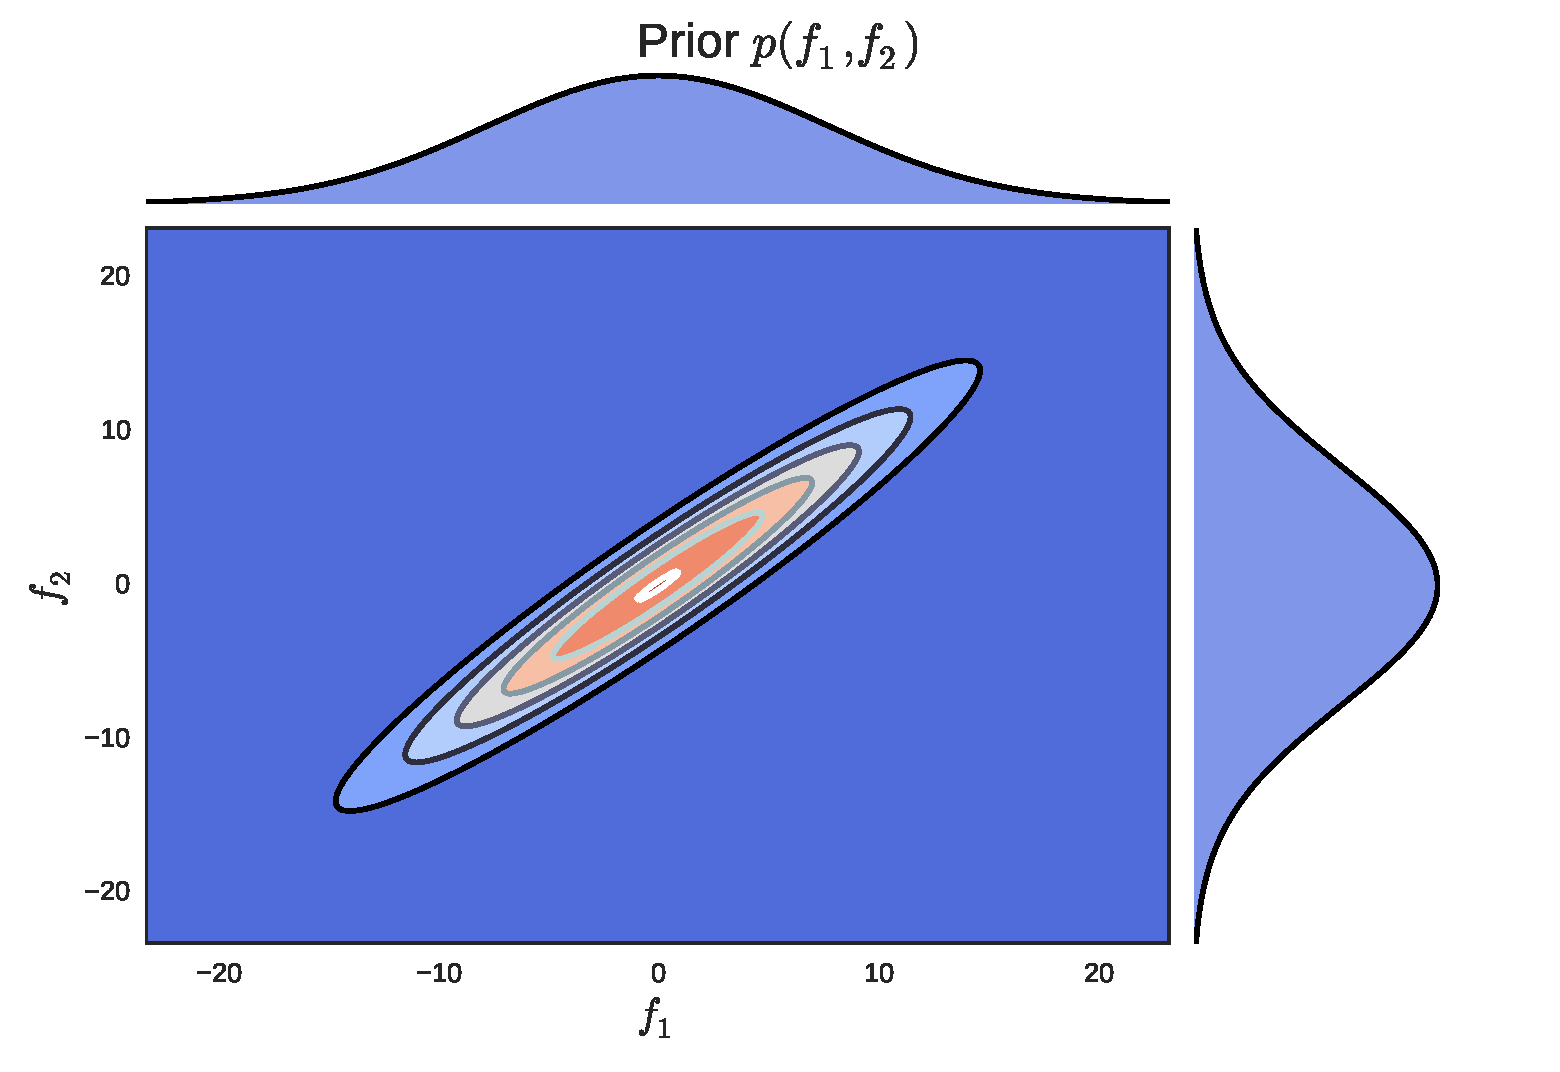
\includegraphics[width=0.55\textwidth]{../diagrams/joint_prior.pdf}
            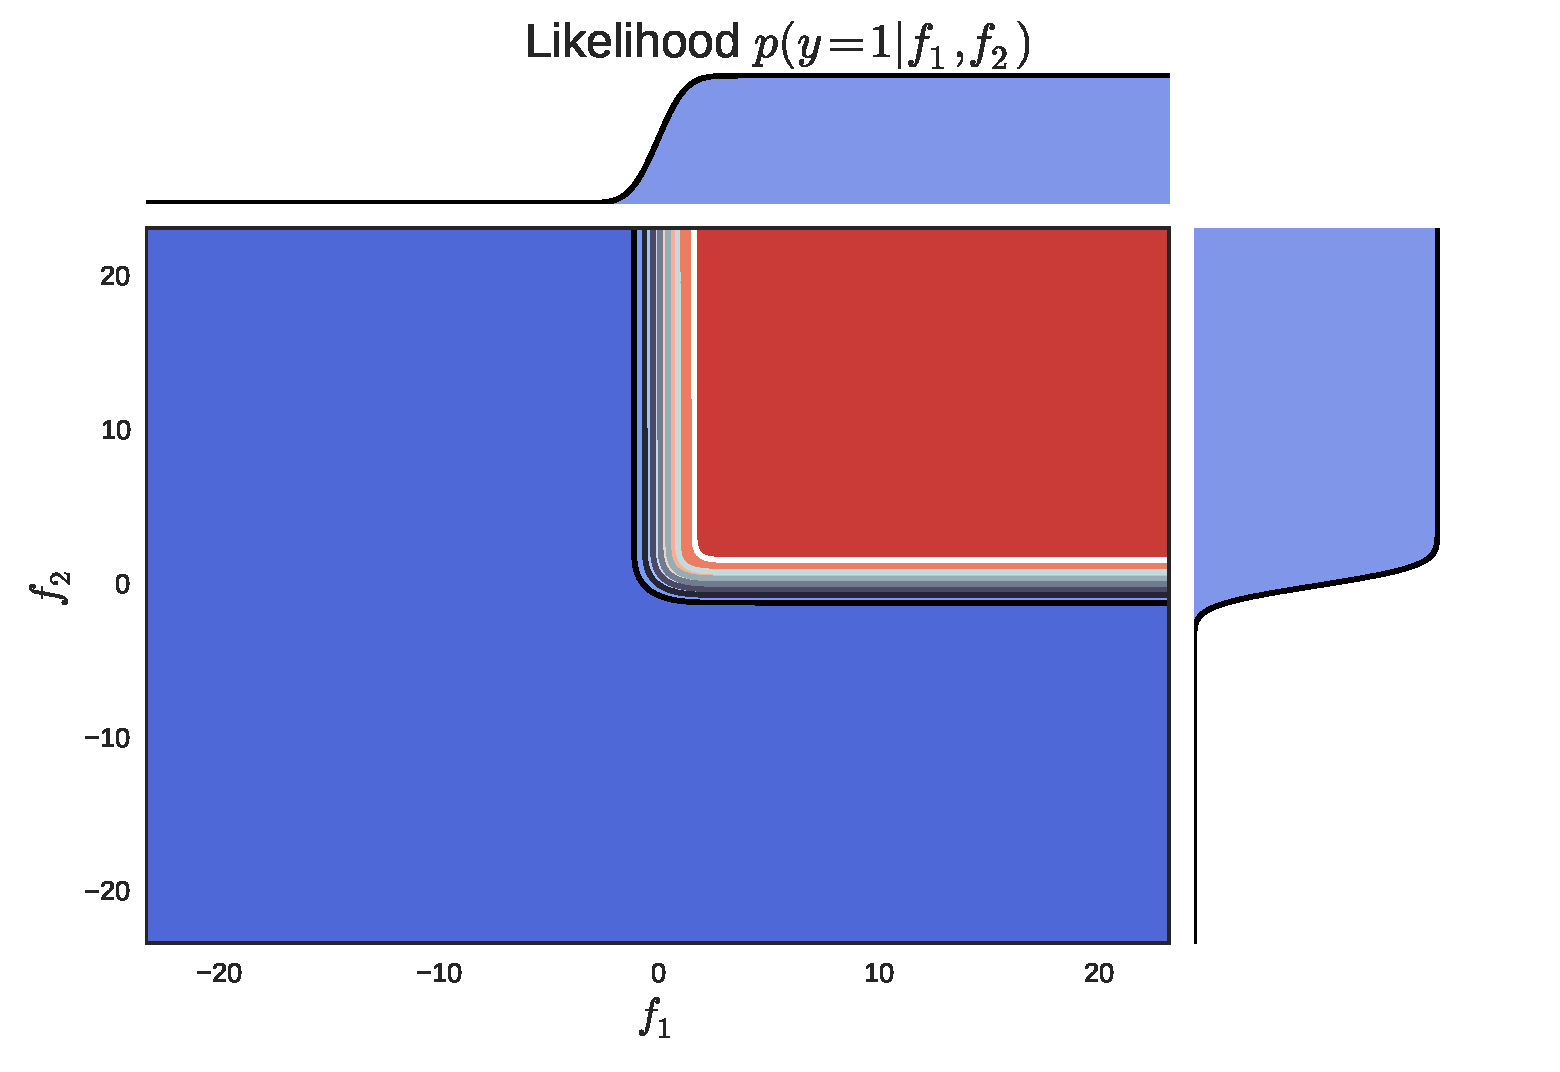
\includegraphics[width=0.55\textwidth]{../diagrams/joint_likelihood.pdf}
        }
        \onslide<2>\centerline{
            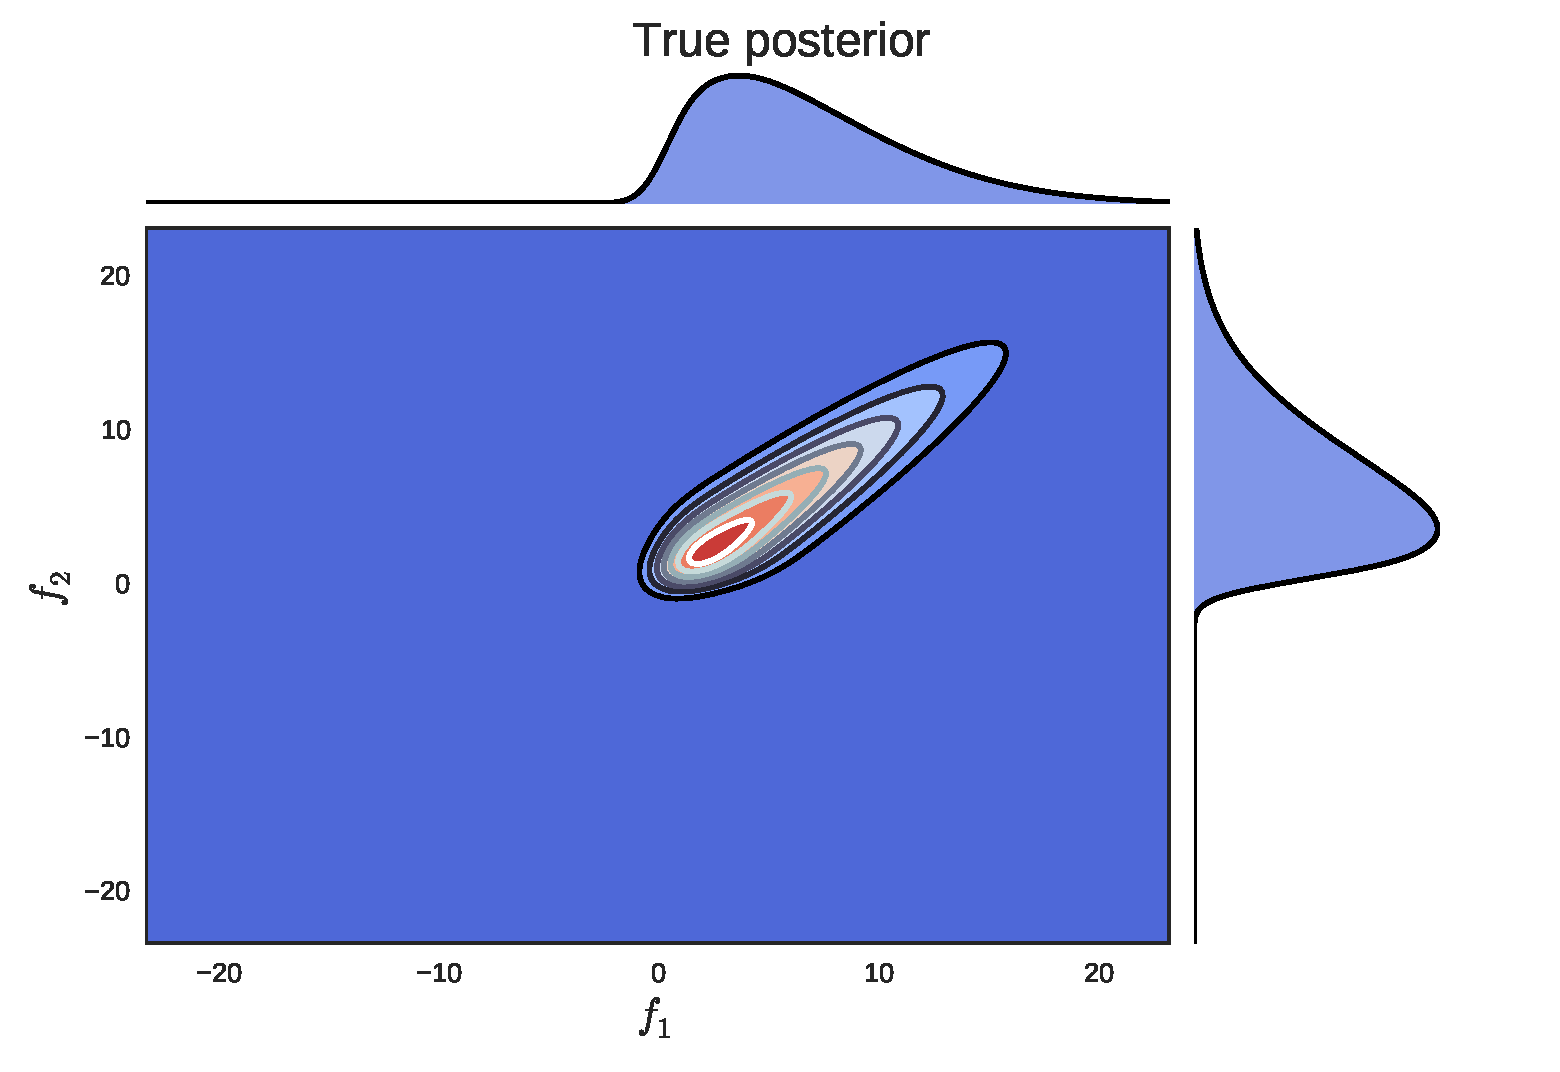
\includegraphics[width=0.55\textwidth]{../diagrams/joint_posterior.pdf}
            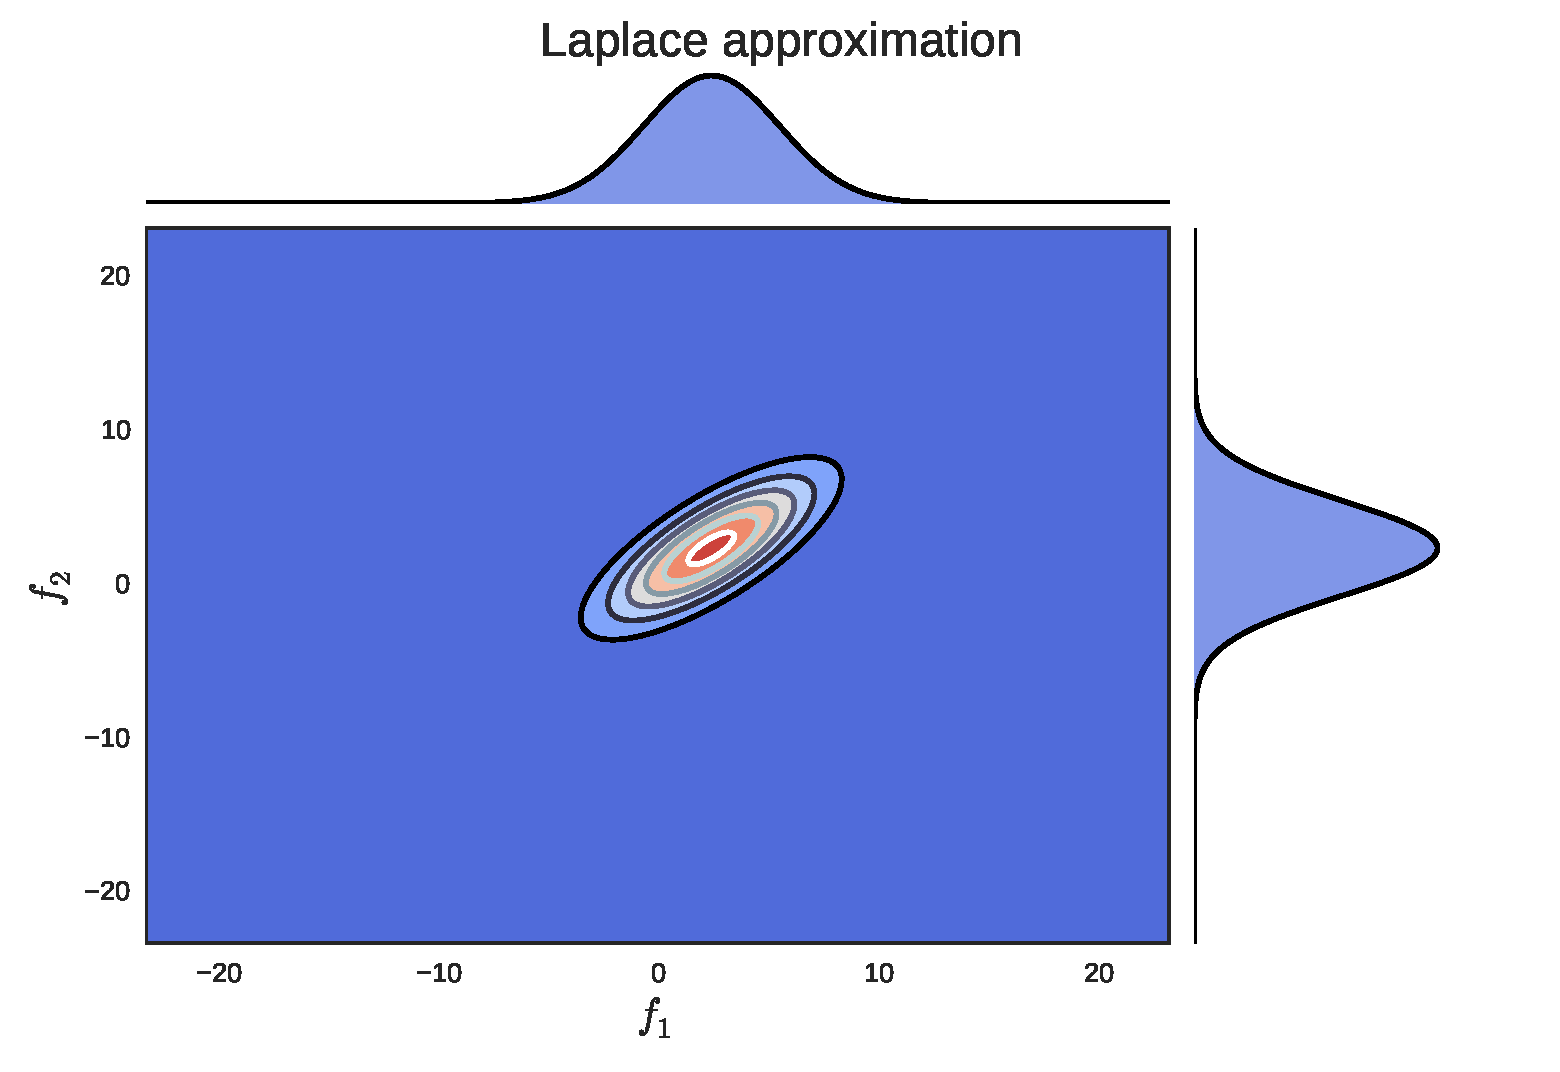
\includegraphics[width=0.55\textwidth]{../diagrams/joint_laplace.pdf}
        }
        \onslide<3>\centerline{
            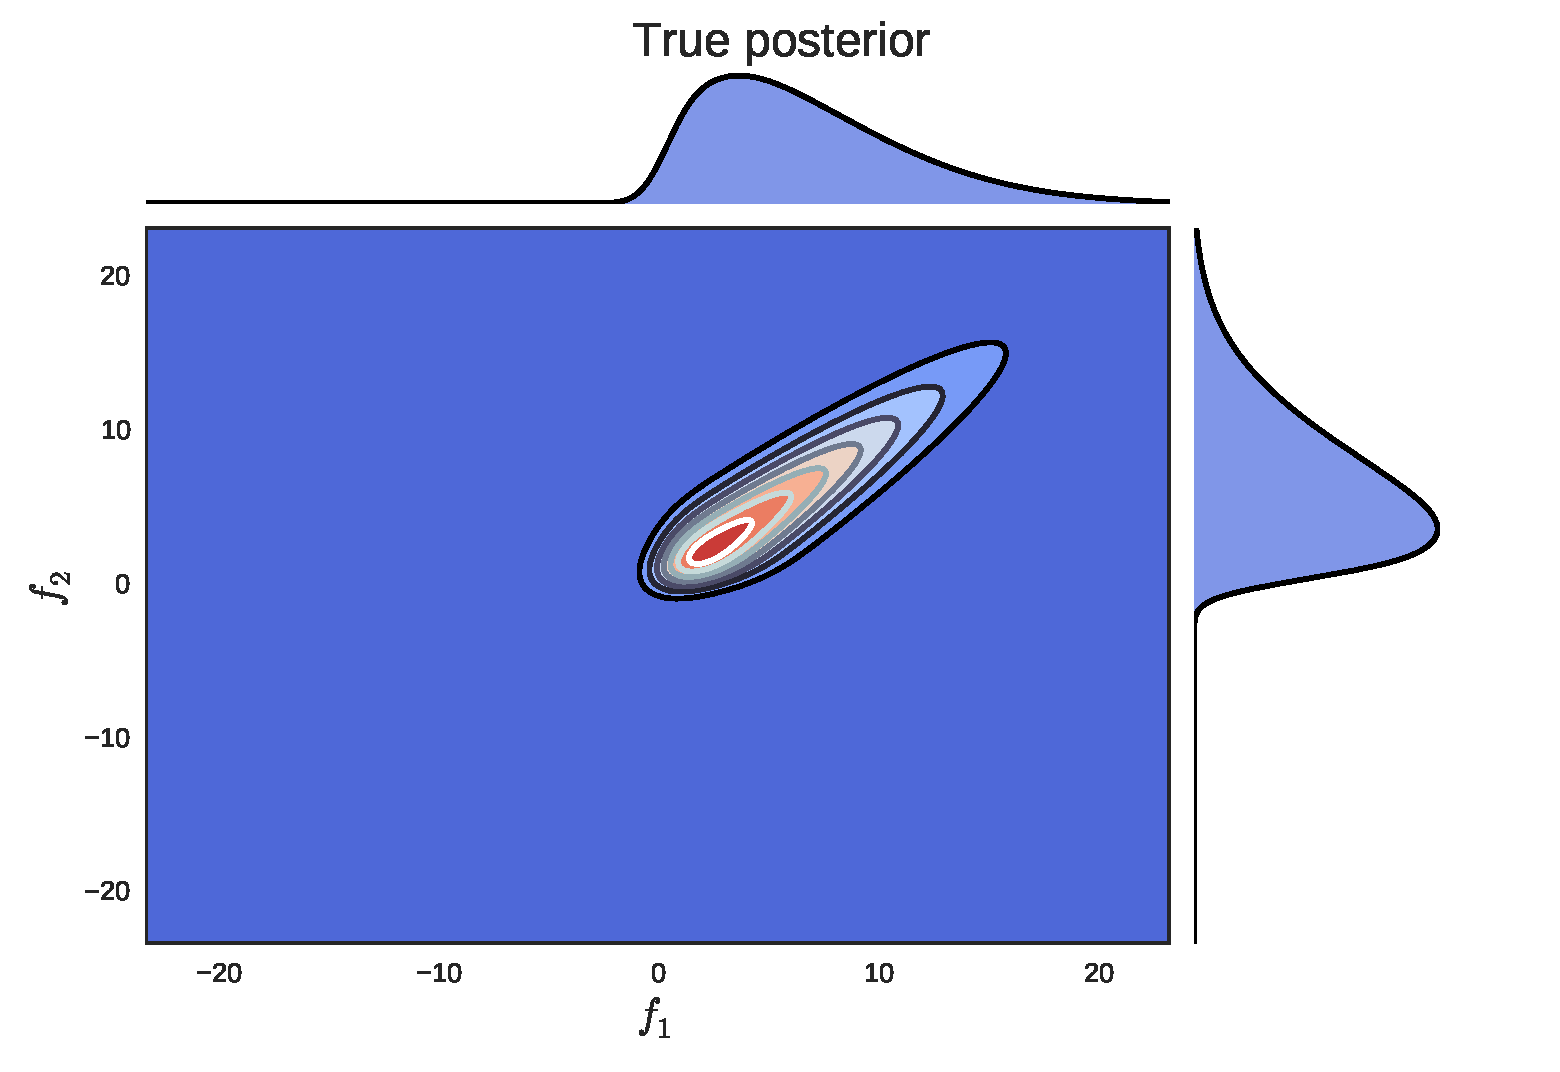
\includegraphics[width=0.55\textwidth]{../diagrams/joint_posterior.pdf}
            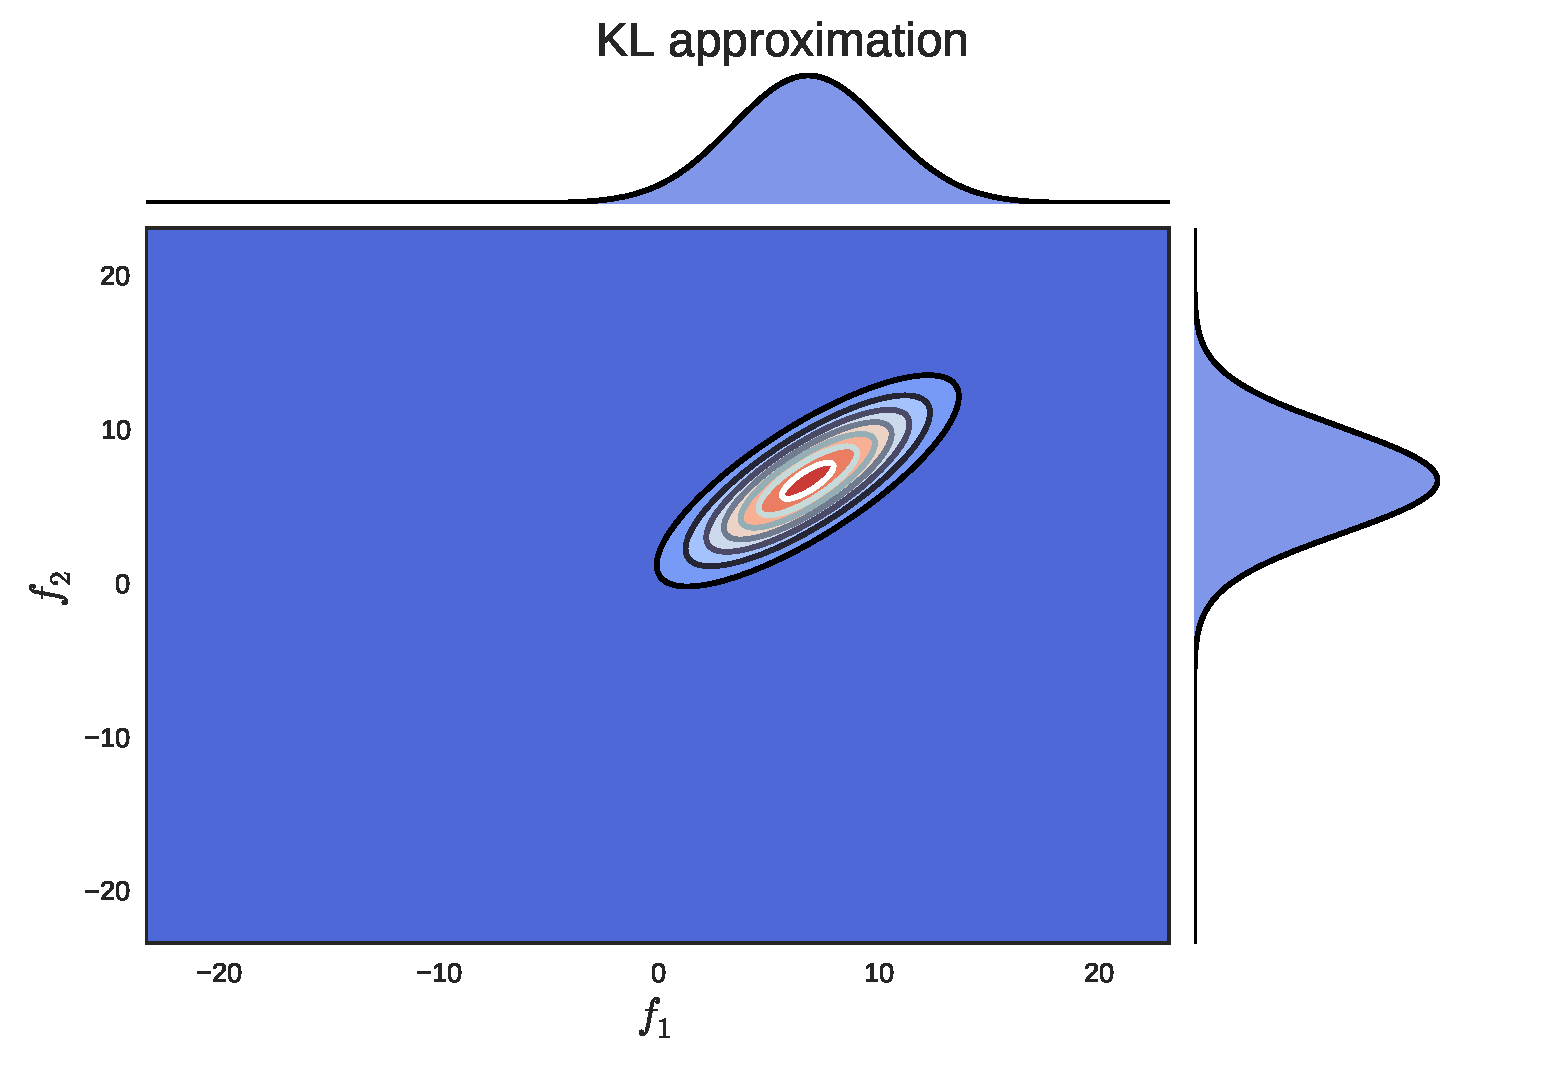
\includegraphics[width=0.55\textwidth]{../diagrams/joint_kl.pdf}
        }
        \onslide<4>\centerline{
            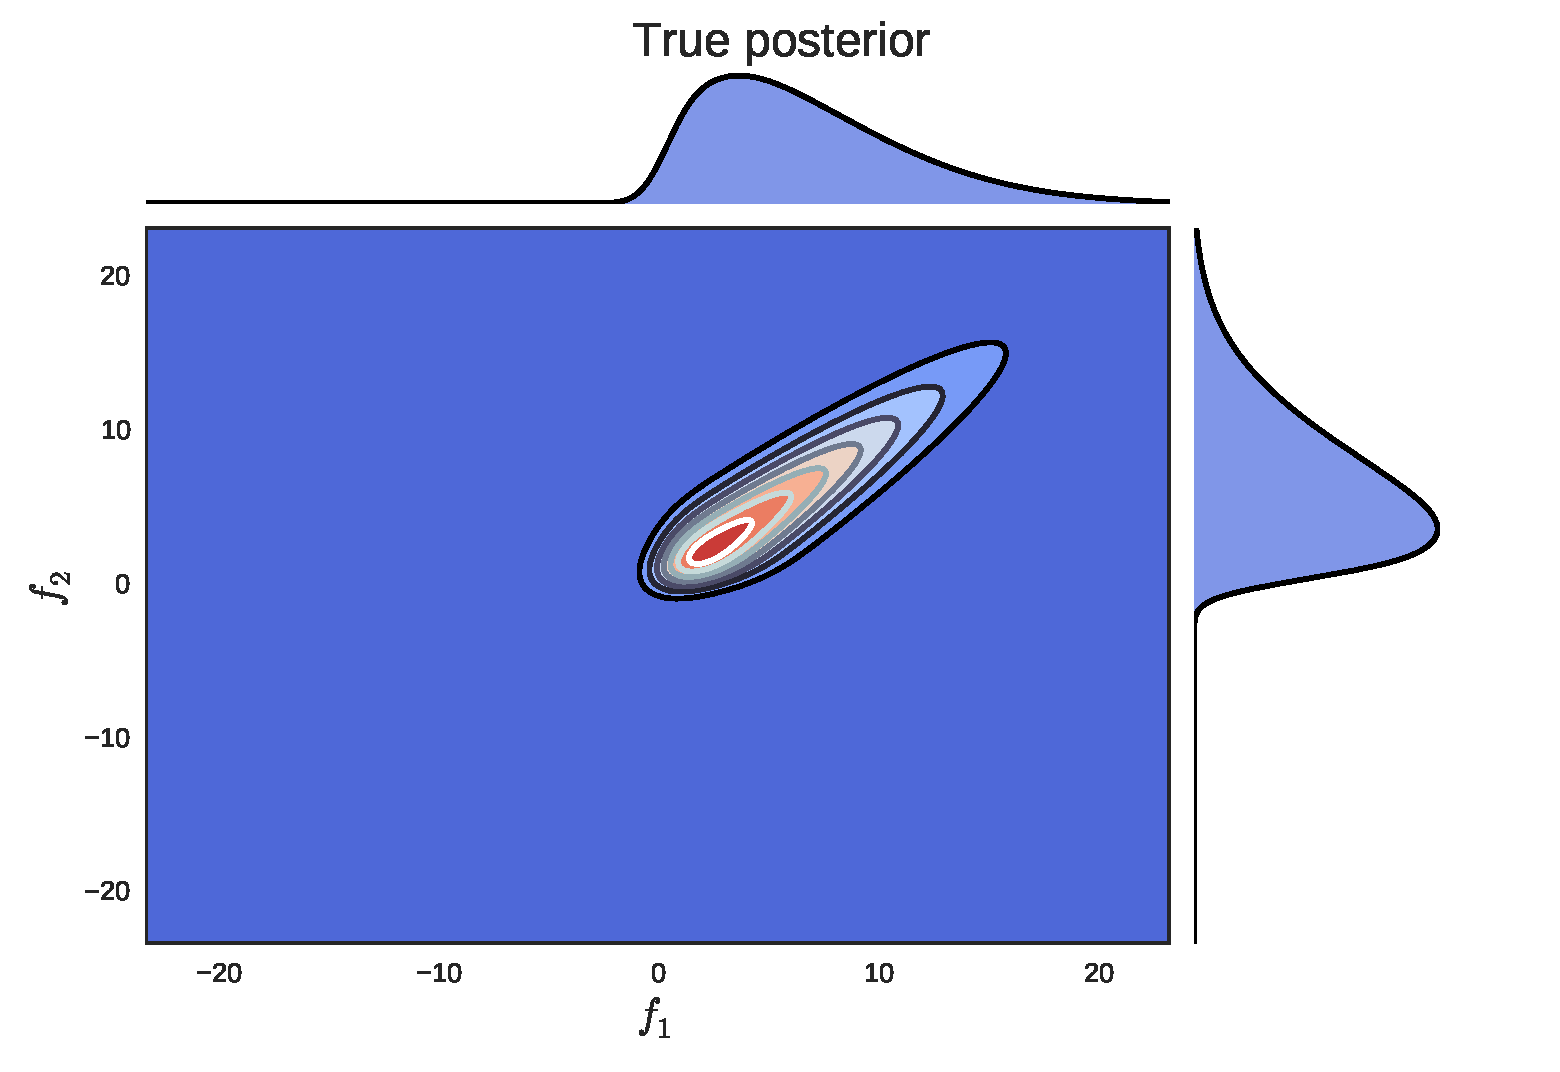
\includegraphics[width=0.55\textwidth]{../diagrams/joint_posterior.pdf}
            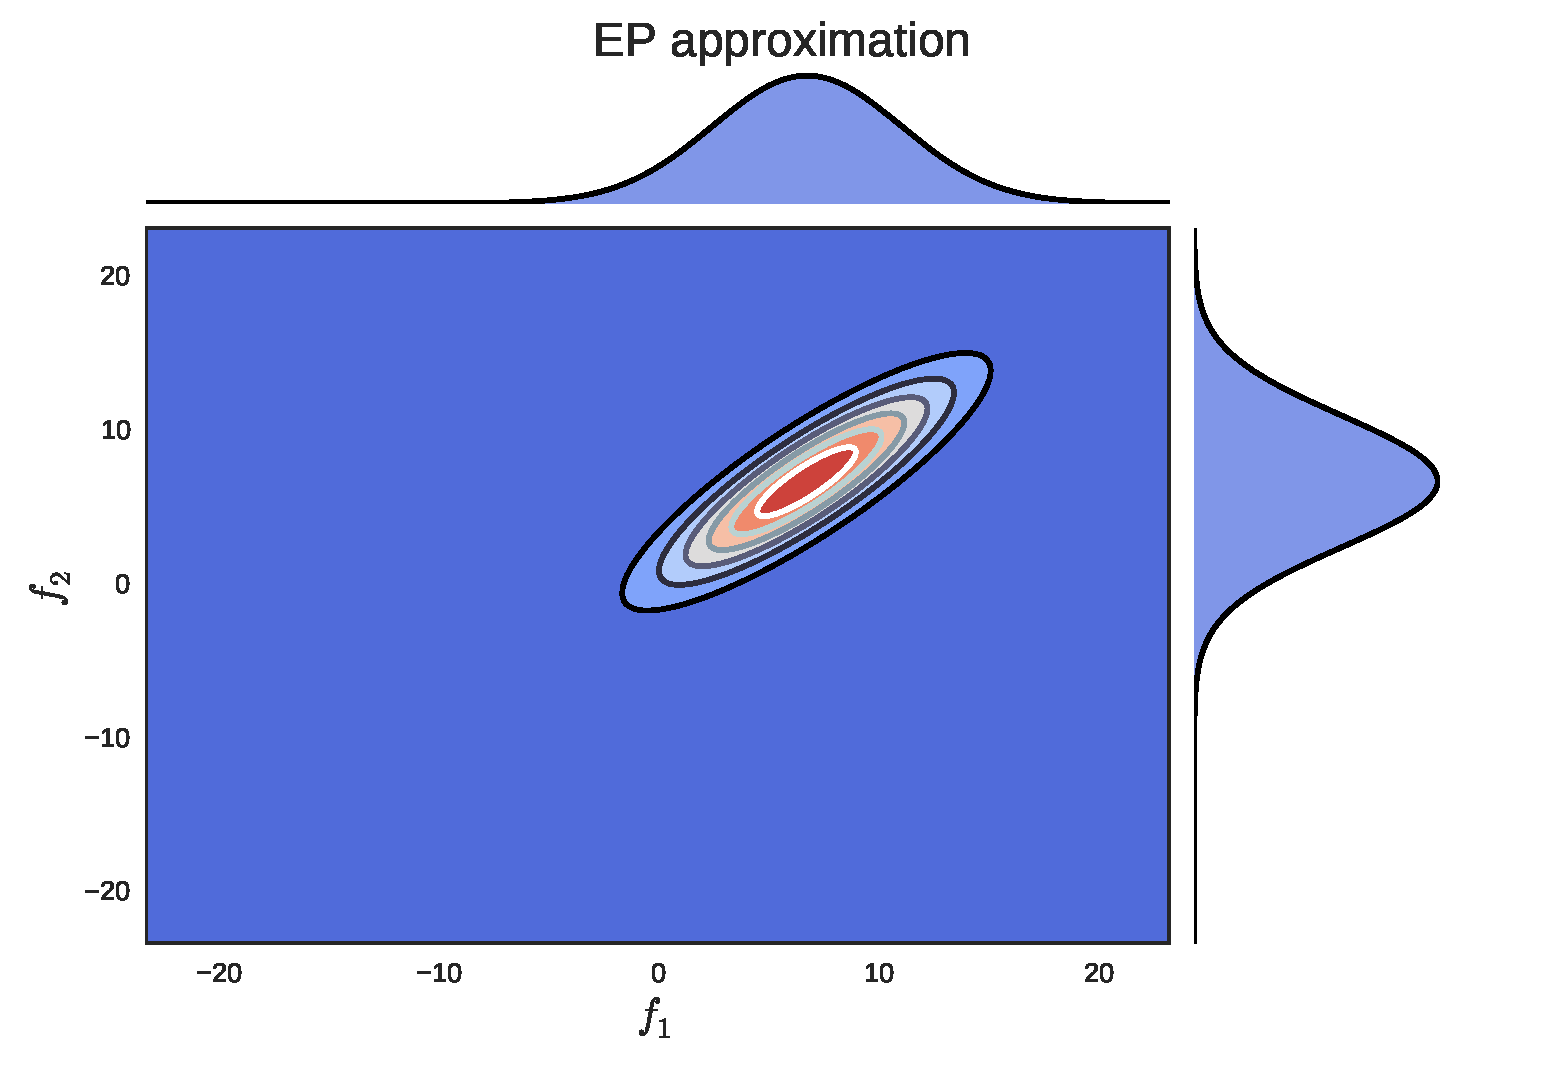
\includegraphics[width=0.55\textwidth]{../diagrams/joint_ep.pdf}
        }
    \end{overprint}
    \begin{overprint}
        \onslide<1> \begin{itemize}
            \item Gaussian prior between two function values $\{\fV_{1}, \fV_{2}\}$, at $\{\xV_{1}, \xV_{2}\}$ respectively. 
            \item Bernoulli likelihood, $\yV_{1} = 1$ and $\yV_{2} = 1$.\end{itemize}
        \onslide<2> \begin{itemize}
            \item $p(\fV|\yV) \propto \frac{p(\yV|\fV)p(\fV)}{p(\yV)}$
            \item True posterior is non-Gaussian.
            \item Laplace approximates with a Gaussian at the mode of the posterior.
        \end{itemize}
        \onslide<3> \begin{itemize}
            \item True posterior is non-Gaussian. 
            \item VB approximate with a Gaussian that has minimal KL divergence, $\KL{q(\fV)}{p(\fV|\yV)}$. 
            \item This leads to distributions that avoid regions in which $p(\fV|\yV)$ is small. 
            \item It has a large penality for assigning density where there is none.
        \end{itemize}
        \onslide<4> \begin{itemize}
            \item True posterior is non-Gaussian. 
            \item EP tends to try and put density where $p(\fV|\yV)$ is large
            \item Cares less about assigning density density where there is none. Contrasts to VB method.
        \end{itemize}
    \end{overprint}
}

\frame{
    \frametitle{Comparing posterior marginal approximations}
        \hspace{0.2em}
        \centerline{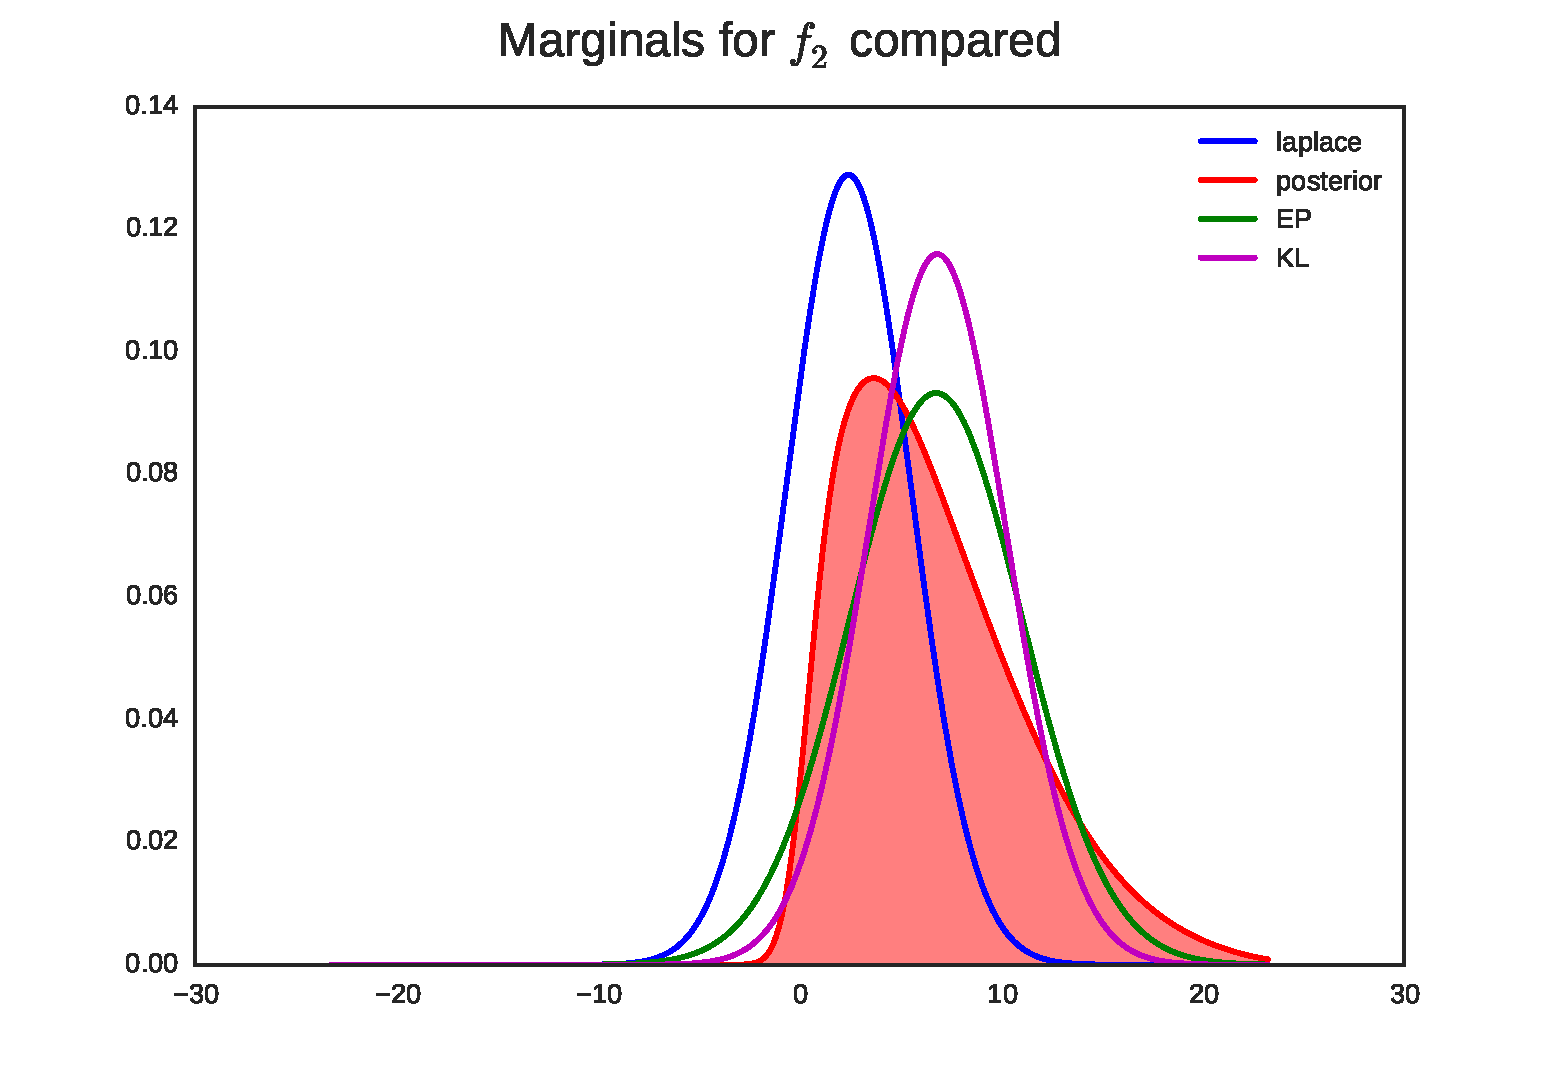
\includegraphics[width=0.6\textwidth,trim={0 1.7cm 0.5cm 0},clip]{../diagrams/marginals.pdf}}
        \hspace{-4em}
        \begin{itemize}
            \item Laplace: Poor approximation.
            \item VB: Avoids assigning density to areas where there is none, at the expense of areas where there is some (right tail).
            \item EP: Assigns density to areas with density, at the expense of areas where there is none (left tail).
        \end{itemize}
}
\frame{
    \frametitle{Pros - Cons - When - Laplace}
    Laplace approximation 
    \begin{itemize}
        \item Pros \begin{itemize}
                \item Very fast.
            \end{itemize}
        \item Cons \begin{itemize}
                \item Poor approximation if the mode does not well describe the posterior, for example Bernoulli likelihood.
            \end{itemize}
        \item When \begin{itemize}
                \item When the posterior \emph{is} well characterized by its mode, for example Poisson.
            \end{itemize}
    \end{itemize}
}

\frame{
    \frametitle{Pros - Cons - When - VB}
    Variational Bayes
    \begin{itemize}
        \item Pros \begin{itemize}
                \item Principled in that it we are directly optimizing a measure of divergence between an approximation and true distribution.
                \item Lends itself to sparse extensions.
                %\item Can be relatively quick, and lends it self to sparse approximations~\citep{Hensman:class15}.
            \end{itemize}
        \item Cons \begin{itemize}
                \item Requires factorizing likelihoods to avoid $\numData$ dimensional integral.
                \item As seen, can result in underestimating the variance, i.e.\ becomes overconfident.
                %\item Often requires numerical quadrature as part of inference, though in practice this can be very accurate.
            \end{itemize}
        \item When \begin{itemize}
                \item Applicable to a range of likelihoods, but is known in some cases to underestimate variance, might need to be careful if you wish to be conservative with predictive uncertainty.
                \item In conjunction with sparse methods.
            \end{itemize}
    \end{itemize}
}

\frame{
    \frametitle{Pros - Cons - When - EP}
    EP method
    \begin{itemize}
        \item Pros \begin{itemize}
                \item Very effective for certain likelihoods (classification).
                \item Also lends itself to sparse approximations.
            \end{itemize}
        \item Cons \begin{itemize}
                \item Standard algorithm is slow though possible to extend to sparse case. 
                \item Convergence issues for some likelihoods.
                \item Must be able to match moments.
            \end{itemize}
        \item When \begin{itemize}
                \item Binary data~\citep{Nickisch:class08,Kuss:robust06}, perhaps with truncated likelihood (censored data)~\citep{Vanhatalo:gpstuff15}.
                \item In conjunction with sparse methods.
            \end{itemize}
    \end{itemize}
}

\frame{
    \frametitle{Pros - Cons - When - MCMC}
    MCMC methods
    \begin{itemize}
        \item Pros \begin{itemize}
                \item Theoretical limit gives true distribution
            \end{itemize}
        \item Cons \begin{itemize}
                \item Can be very slow
            \end{itemize}
        \item When \begin{itemize}
                \item If time is not an issue, but exact accuracy is.
                \item If you are unsure whether a different approximation is appropriate, can be used as a ``ground truth''
            \end{itemize}
    \end{itemize}
}

\frame{
    \frametitle{Conclusion}
    \begin{itemize}
        \item Many real world tasks require non-Gaussian observation models.
        \item Non-Gaussian likelihoods cause complications in applying our framework.
        \item Several different ways to deal with the problem. Many are based on Gaussian approximations.
        \item Different methods have their own advantages and disadvantages.
    \end{itemize}
}

\frame{
    \frametitle{Questions}
    \begin{center}
        {\large Thanks for listening.\\
            \vspace{2em}Any questions?\\
        }
        \vspace{4em}
    \end{center}
}

\frame{
    \frametitle{Bonus - Hetroscedastic likelihoods}
    \centerline{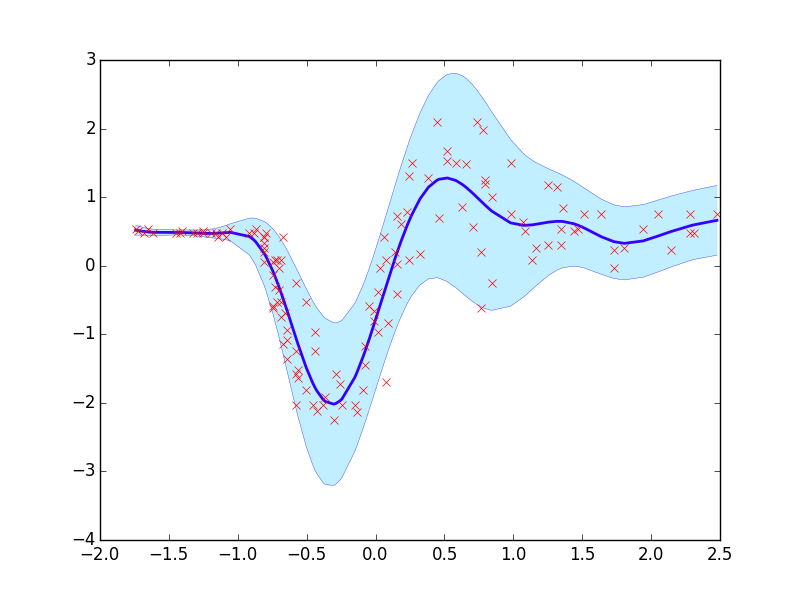
\includegraphics[width=0.7\textwidth]{../diagrams/silverman_het_gauss.png}}
    \begin{itemize}
        \item Likelihood whos parameters are governed by two known functions, $\fV$ and $\mathbf{g}$.
        \item $p(\yV|\fV, \mathbf{g}) = \gaussianDist{\yV}{\mu=\fV}{\sigma^{2}=\exp(\mathbf{g})}$
    \end{itemize}
}

\frame{
    \frametitle{Bonus - non-Gaussian hetroscedastic likelihoods}
    \begin{center}
    \resizebox{1.0\textwidth}{!}{%
        % This file was created by matplotlib v0.1.0.
% Copyright (c) 2010--2014, Nico Schlömer <nico.schloemer@gmail.com>
% All rights reserved.
% 
% The lastest updates can be retrieved from
% 
% https://github.com/nschloe/matplotlib2tikz
% 
% where you can also submit bug reports and leavecomments.
% 
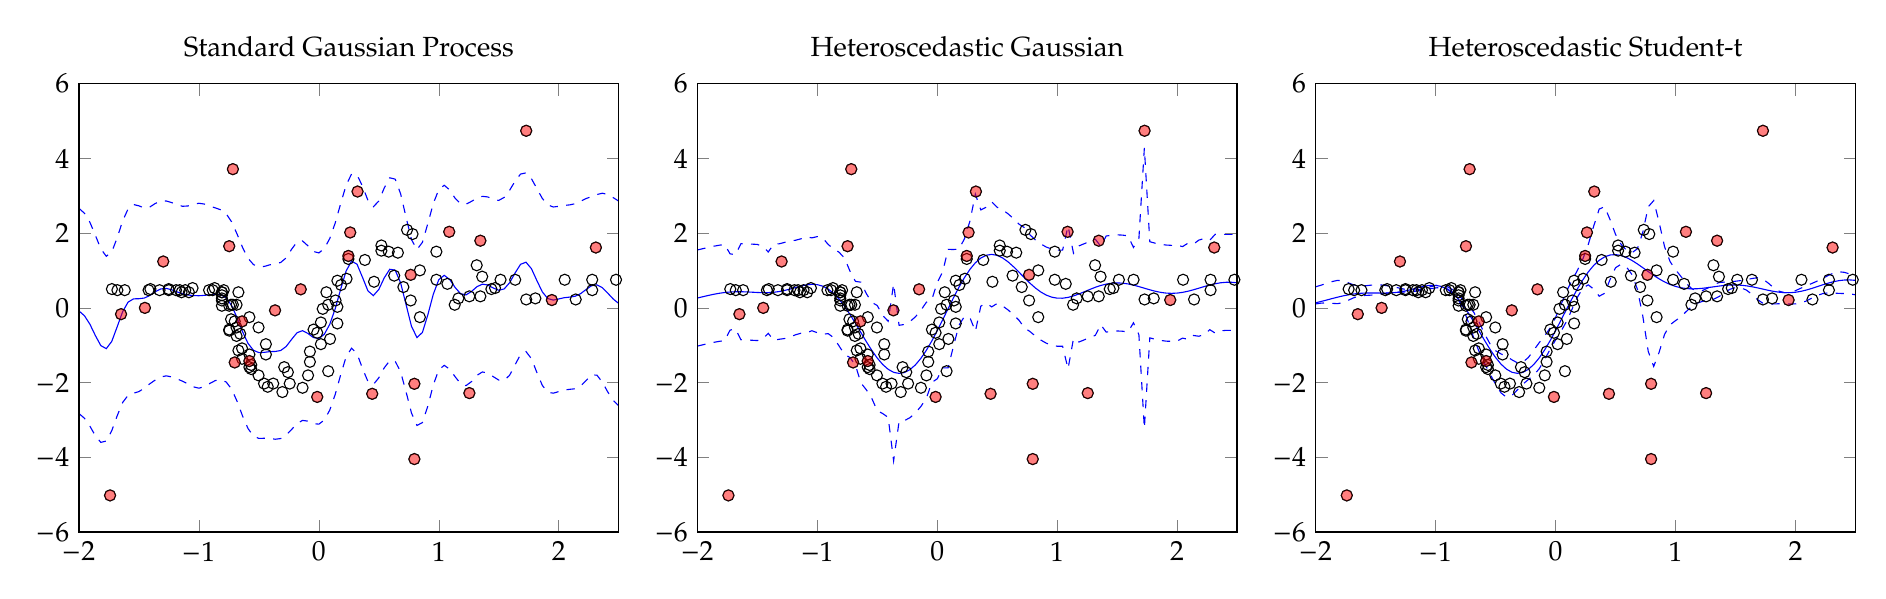
\begin{tikzpicture}

\begin{groupplot}[group style={group size=3 by 1}]
\nextgroupplot[
title={Standard Gaussian Process},
xmin=-2, xmax=2.5,
ymin=-6, ymax=6,
axis on top
]
\addplot [black, mark=o, mark size=2, only marks]
coordinates {
(-1.74116352672168,-5.0195403780745)
(-1.72587604658873,0.503652715299266)
(-1.68001360618987,0.474570898203498)
(-1.64943864592396,-0.168155449259482)
(-1.61886368565805,0.474570898203498)
(-1.45070140419556,0.000133410180054608)
(-1.42012644392965,0.474570898203498)
(-1.4048389637967,0.503652715299266)
(-1.32840156313193,0.474570898203498)
(-1.29782660286602,1.24169382547938)
(-1.25196416246716,0.474570898203498)
(-1.25196416246716,0.503652715299266)
(-1.19081424193535,0.474570898203498)
(-1.16023928166944,0.474570898203498)
(-1.14495180153648,0.41848453666166)
(-1.11437684127058,0.474570898203498)
(-1.08380188100467,0.41848453666166)
(-1.05322692073876,0.530657259745337)
(-0.915639599542178,0.474570898203498)
(-0.885064639276271,0.474570898203498)
(-0.869777159143317,0.530657259745337)
(-0.808627238611502,0.0570390956142563)
(-0.808627238611502,0.25437999733554)
(-0.808627238611502,0.41848453666166)
(-0.808627238611502,0.41848453666166)
(-0.808627238611502,0.198293635793701)
(-0.808627238611502,0.337470903323449)
(-0.793339758478548,0.474570898203498)
(-0.747477318079687,-0.580683607842944)
(-0.747477318079687,1.65110184686199)
(-0.747477318079687,0.0570390956142563)
(-0.747477318079687,-0.609765424938712)
(-0.732189837946733,-0.304406345433147)
(-0.732189837946733,0.0840436400603267)
(-0.716902357813779,0.0840436400603267)
(-0.716902357813779,3.71332902532434)
(-0.701614877680826,-1.46062918600775)
(-0.701614877680826,-0.360492706974986)
(-0.686327397547872,-0.524597246301106)
(-0.686327397547872,0.0840436400603267)
(-0.686327397547872,-0.751019965118157)
(-0.671039917414918,0.41848453666166)
(-0.671039917414918,-1.13946995061163)
(-0.655752437281964,-0.694933603576319)
(-0.640464957149011,-1.08338358906979)
(-0.640464957149011,-0.362328736646449)
(-0.640464957149011,-1.36173812412929)
(-0.579315036617195,-1.42287784457826)
(-0.579315036617195,-0.248319983891309)
(-0.579315036617195,-1.24748812839591)
(-0.579315036617195,-1.58608357029664)
(-0.564027556484242,-1.63801538653908)
(-0.564027556484242,-1.52791993610511)
(-0.502877635952427,-1.8062744711646)
(-0.502877635952427,-0.524597246301106)
(-0.457015195553566,-2.02646537203256)
(-0.441727715420612,-0.971210865986116)
(-0.441727715420612,-1.24748812839591)
(-0.426440235287658,-2.11163355067017)
(-0.380577794888797,-2.02646537203256)
(-0.365290314755843,-0.0662809637383996)
(-0.304140394224028,-2.25288809084961)
(-0.288852914091074,-1.58608357029664)
(-0.258277953825167,-1.72110629252699)
(-0.242990473692213,-2.02646537203256)
(-0.15126559289449,0.496358900368174)
(-0.135978112761537,-2.13863809511624)
(-0.0901156723626754,-1.8062744711646)
(-0.0748281922297217,-1.1685517677074)
(-0.0748281922297217,-1.4448290301172)
(-0.044253231963814,-0.580683607842944)
(-0.0136782716979066,-0.665851786480551)
(-0.0136782716979066,-2.38342677759337)
(0.0168966885680008,-0.389574524070754)
(0.0168966885680008,-0.971210865986116)
(0.0321841687009548,-0.0260518103736526)
(0.0627591289668622,0.41848453666166)
(0.0780466090998159,0.0840436400603267)
(0.0780466090998159,-1.69410174808092)
(0.0933340892327696,-0.832033598456368)
(0.139196529631631,0.198293635793701)
(0.154484009764585,-0.416579068516824)
(0.154484009764585,0.72799816146662)
(0.154484009764585,0.0279572785184882)
(0.185058970030492,0.613748165733246)
(0.230921410429353,0.779929977709063)
(0.246208890562307,1.39026088822429)
(0.246208890562307,1.30963450338198)
(0.261496370695261,2.01896695219706)
(0.322646291227076,3.11414008455091)
(0.383796211758891,1.28262995893591)
(0.444946132290706,-2.30011960226108)
(0.46023361242366,0.698916344370852)
(0.521383532955475,1.53190267689964)
(0.521383532955475,1.67107994442939)
(0.58253345348729,1.50489813245357)
(0.628395893886151,0.863020883696972)
(0.658970854152058,1.4778935880075)
(0.70483329455092,0.557661804191407)
(0.735408254816827,2.08861174701863)
(0.765983215082735,0.884748398209662)
(0.765983215082735,0.198293635793701)
(0.781270695215689,1.97643902393495)
(0.796558175348642,-4.04698513889632)
(0.796558175348642,-2.03223413224145)
(0.842420615747504,-0.248319983891309)
(0.842420615747504,1.00427542387642)
(0.980007936944087,0.752925433262993)
(0.980007936944087,1.50489813245357)
(1.07173281774181,0.642829982829014)
(1.08702029787476,2.03636910171517)
(1.13288273827363,0.0840436400603267)
(1.16345769853953,0.25437999733554)
(1.25518257933726,-2.28100346605642)
(1.25518257933726,0.308389086227681)
(1.31633249986907,1.14137541875647)
(1.34690746013498,0.308389086227681)
(1.34690746013498,1.79827844539709)
(1.36219494026793,0.836016339250902)
(1.4386323409327,0.503652715299266)
(1.46920730119861,0.530657259745337)
(1.51506974159747,0.752925433262993)
(1.6373695826611,0.752925433262993)
(1.72909446345882,4.7408922404752)
(1.72909446345882,0.225298180239772)
(1.80553186412359,0.25437999733554)
(1.94311918532017,0.210000324231941)
(2.05013154625085,0.752925433262993)
(2.14185642704857,0.225298180239772)
(2.27944374824516,0.474570898203498)
(2.27944374824516,0.752925433262993)
(2.31001870851106,1.61551969868625)
(2.47818098997356,0.752925433262993)

};
\addplot [blue]
coordinates {
(-2,-0.0832449691300349)
(-1.95454545454546,-0.211022687739565)
(-1.90909090909091,-0.438076672322211)
(-1.86363636363636,-0.740621325305255)
(-1.81818181818182,-1.00997233941343)
(-1.77272727272727,-1.09117268488707)
(-1.72727272727273,-0.89851384560715)
(-1.68181818181818,-0.505841302493057)
(-1.63636363636364,-0.102284815301943)
(-1.59090909090909,0.154589249426602)
(-1.54545454545455,0.241737557141824)
(-1.5,0.245541240793436)
(-1.45454545454546,0.264024265728379)
(-1.40909090909091,0.335487699159274)
(-1.36363636363636,0.43347436369573)
(-1.31818181818182,0.50628841437746)
(-1.27272727272727,0.521493669214114)
(-1.22727272727273,0.485183342866501)
(-1.18181818181818,0.428158546063383)
(-1.13636363636364,0.378084689912664)
(-1.09090909090909,0.345187408912885)
(-1.04545454545455,0.328377978597273)
(-1,0.325570204038187)
(-0.954545454545455,0.334976248215962)
(-0.90909090909091,0.351721522993558)
(-0.863636363636364,0.365380132810659)
(-0.818181818181819,0.352486699942799)
(-0.772727272727274,0.267972402497669)
(-0.727272727272728,0.0632324452927146)
(-0.681818181818183,-0.263219274738743)
(-0.636363636363637,-0.636921399690413)
(-0.590909090909092,-0.949845671502326)
(-0.545454545454546,-1.13512331815528)
(-0.500000000000001,-1.19759491311146)
(-0.454545454545455,-1.18967348556363)
(-0.40909090909091,-1.17081880881071)
(-0.363636363636364,-1.16631495067396)
(-0.318181818181819,-1.14105337992759)
(-0.272727272727274,-1.03350107503071)
(-0.227272727272728,-0.842817467369431)
(-0.181818181818183,-0.664940367869903)
(-0.136363636363637,-0.609402074093805)
(-0.0909090909090917,-0.68548501492022)
(-0.0454545454545463,-0.793894593535485)
(-8.88178419700125e-16,-0.820313590235041)
(0.0454545454545445,-0.70671557709846)
(0.0909090909090899,-0.439511002117818)
(0.136363636363635,-0.0220209899947078)
(0.181818181818181,0.498760071901329)
(0.227272727272727,0.987641882947926)
(0.272727272727272,1.25179234841586)
(0.318181818181817,1.17000019689518)
(0.363636363636363,0.819319764237387)
(0.409090909090908,0.455547055789174)
(0.454545454545454,0.328279395712209)
(0.499999999999999,0.49452950643933)
(0.545454545454545,0.804120175151375)
(0.59090909090909,1.03351784915993)
(0.636363636363635,1.0108239051344)
(0.681818181818181,0.669816528311532)
(0.727272727272727,0.0887358935994043)
(0.772727272727272,-0.49609200886851)
(0.818181818181817,-0.794115630364363)
(0.863636363636363,-0.656381459329699)
(0.909090909090908,-0.182247587731029)
(0.954545454545454,0.368336049542666)
(0.999999999999999,0.75484760565484)
(1.04545454545454,0.87203034751642)
(1.09090909090909,0.75889230326649)
(1.13636363636364,0.545826467242735)
(1.18181818181818,0.379323125972694)
(1.22727272727273,0.347328050795704)
(1.27272727272727,0.438875316741052)
(1.31818181818182,0.566266952219044)
(1.36363636363636,0.635704550600717)
(1.40909090909091,0.612017316990164)
(1.45454545454545,0.531997823819954)
(1.5,0.472101373229143)
(1.54545454545454,0.507137823957941)
(1.59090909090909,0.674007041954527)
(1.63636363636364,0.934777905418019)
(1.68181818181818,1.16625138779793)
(1.72727272727273,1.22294064745356)
(1.77272727272727,1.04890842524018)
(1.81818181818182,0.730364060818174)
(1.86363636363636,0.426604226033894)
(1.90909090909091,0.250067791452052)
(1.95454545454545,0.208699036135048)
(2,0.238522470801102)
(2.04545454545454,0.272410739834417)
(2.09090909090909,0.288093935163897)
(2.13636363636364,0.311286018960155)
(2.18181818181818,0.378302537146629)
(2.22727272727273,0.488665281342762)
(2.27272727272727,0.590664492090098)
(2.31818181818182,0.61744527075547)
(2.36363636363636,0.54143844307459)
(2.40909090909091,0.394547560287917)
(2.45454545454545,0.23833872226331)
(2.5,0.11930332541959)

};
\addplot [blue, dashed]
coordinates {
(-2,2.66359286845116)
(-1.95454545454546,2.53253428846944)
(-1.90909090909091,2.2904730265806)
(-1.86363636363636,1.94202330581676)
(-1.81818181818182,1.58019125919897)
(-1.77272727272727,1.38161550274139)
(-1.72727272727273,1.49280609515439)
(-1.68181818181818,1.87702798938661)
(-1.63636363636364,2.3275655461609)
(-1.59090909090909,2.64880237995971)
(-1.54545454545455,2.76701797886225)
(-1.5,2.73096784146311)
(-1.45454545454546,2.67261254916238)
(-1.40909090909091,2.7014868629671)
(-1.36363636363636,2.7956991573084)
(-1.31818181818182,2.86118845394684)
(-1.27272727272727,2.86186745905352)
(-1.22727272727273,2.8182946309885)
(-1.18181818181818,2.75861387351977)
(-1.13636363636364,2.71941559879649)
(-1.09090909090909,2.72844394643408)
(-1.04545454545455,2.77140333433993)
(-1,2.80026048245035)
(-0.954545454545455,2.77921537461203)
(-0.90909090909091,2.72526798912276)
(-0.863636363636364,2.6763075671157)
(-0.818181818181819,2.62619601675552)
(-0.772727272727274,2.52051499205912)
(-0.727272727272728,2.30198958439706)
(-0.681818181818183,1.9751513112836)
(-0.636363636363637,1.61926822061445)
(-0.590909090909092,1.32912795449008)
(-0.545454545454546,1.15908972040915)
(-0.500000000000001,1.09942774634186)
(-0.454545454545455,1.11010574958638)
(-0.40909090909091,1.15239182137698)
(-0.363636363636364,1.18320600177517)
(-0.318181818181819,1.21533951116879)
(-0.272727272727274,1.33838529630081)
(-0.227272727272728,1.56877289371508)
(-0.181818181818183,1.76710511990075)
(-0.136363636363637,1.79286812512184)
(-0.0909090909090917,1.66066898483102)
(-0.0454545454545463,1.51060699136141)
(-8.88178419700125e-16,1.47170561822607)
(0.0454545454545445,1.58782484089415)
(0.0909090909090899,1.85673773774304)
(0.136363636363635,2.27223388628461)
(0.181818181818181,2.79034146125257)
(0.227272727272727,3.28455314886889)
(0.272727272727272,3.58262701944065)
(0.318181818181817,3.56386020532088)
(0.363636363636363,3.2580071987828)
(0.409090909090908,2.8800943056111)
(0.454545454545454,2.70665177027845)
(0.499999999999999,2.8605729481318)
(0.545454545454545,3.21128536665316)
(0.59090909090909,3.48161991388812)
(0.636363636363635,3.44690908435528)
(0.681818181818181,3.05411203443997)
(0.727272727272727,2.4258243736148)
(0.772727272727272,1.82562286547411)
(0.818181818181817,1.55896973723164)
(0.863636363636363,1.75647590030665)
(0.909090909090908,2.2608918069675)
(0.954545454545454,2.79579706660054)
(0.999999999999999,3.16679414015022)
(1.04545454545454,3.28249033794198)
(1.09090909090909,3.15670439017002)
(1.13636363636364,2.93457476659553)
(1.18181818181818,2.78691326869348)
(1.22727272727273,2.77503931830152)
(1.27272727272727,2.85129808856265)
(1.31818181818182,2.93864663774266)
(1.36363636363636,2.9861534636498)
(1.40909090909091,2.96920184732614)
(1.45454545454545,2.9052372717744)
(1.5,2.87632530266762)
(1.54545454545454,2.95766634570294)
(1.59090909090909,3.14922202043234)
(1.63636363636364,3.39137204774337)
(1.68181818181818,3.58195278018571)
(1.72727272727273,3.61377458808357)
(1.77272727272727,3.45836166179959)
(1.81818181818182,3.19151381520167)
(1.86363636363636,2.92906372042299)
(1.90909090909091,2.7570109074167)
(1.95454545454545,2.70066025412495)
(2,2.71827990508249)
(2.04545454545454,2.74342892862386)
(2.09090909090909,2.75640530378297)
(2.13636363636364,2.7879306571441)
(2.18181818181818,2.85406342387524)
(2.22727272727273,2.92436691636176)
(2.27272727272727,2.97857247226899)
(2.31818181818182,3.03315198960732)
(2.36363636363636,3.06884768761243)
(2.40909090909091,3.03866069537309)
(2.45454545454545,2.95130635350032)
(2.5,2.85856823104117)

};
\addplot [blue, dashed]
coordinates {
(-2,-2.83008280671123)
(-1.95454545454546,-2.95457966394857)
(-1.90909090909091,-3.16662637122503)
(-1.86363636363636,-3.42326595642727)
(-1.81818181818182,-3.60013593802582)
(-1.77272727272727,-3.56396087251552)
(-1.72727272727273,-3.28983378636869)
(-1.68181818181818,-2.88871059437273)
(-1.63636363636364,-2.53213517676478)
(-1.59090909090909,-2.33962388110651)
(-1.54545454545455,-2.2835428645786)
(-1.5,-2.23988535987624)
(-1.45454545454546,-2.14456401770562)
(-1.40909090909091,-2.03051146464855)
(-1.36363636363636,-1.92875042991694)
(-1.31818181818182,-1.84861162519192)
(-1.27272727272727,-1.81888012062529)
(-1.22727272727273,-1.8479279452555)
(-1.18181818181818,-1.90229678139301)
(-1.13636363636364,-1.96324621897117)
(-1.09090909090909,-2.03806912860831)
(-1.04545454545455,-2.11464737714539)
(-1,-2.14912007437398)
(-0.954545454545455,-2.1092628781801)
(-0.90909090909091,-2.02182494313564)
(-0.863636363636364,-1.94554730149438)
(-0.818181818181819,-1.92122261686992)
(-0.772727272727274,-1.98457018706378)
(-0.727272727272728,-2.17552469381164)
(-0.681818181818183,-2.50158986076108)
(-0.636363636363637,-2.89311101999528)
(-0.590909090909092,-3.22881929749473)
(-0.545454545454546,-3.42933635671971)
(-0.500000000000001,-3.49461757256477)
(-0.454545454545455,-3.48945272071363)
(-0.40909090909091,-3.4940294389984)
(-0.363636363636364,-3.51583590312308)
(-0.318181818181819,-3.49744627102397)
(-0.272727272727274,-3.40538744636222)
(-0.227272727272728,-3.25440782845394)
(-0.181818181818183,-3.09698585564056)
(-0.136363636363637,-3.01167227330945)
(-0.0909090909090917,-3.03163901467146)
(-0.0454545454545463,-3.09839617843239)
(-8.88178419700125e-16,-3.11233279869615)
(0.0454545454545445,-3.00125599509107)
(0.0909090909090899,-2.73575974197868)
(0.136363636363635,-2.31627586627403)
(0.181818181818181,-1.79282131744991)
(0.227272727272727,-1.30926938297304)
(0.272727272727272,-1.07904232260894)
(0.318181818181817,-1.22385981153053)
(0.363636363636363,-1.61936767030803)
(0.409090909090908,-1.96900019403276)
(0.454545454545454,-2.05009297885403)
(0.499999999999999,-1.87151393525314)
(0.545454545454545,-1.60304501635041)
(0.59090909090909,-1.41458421556826)
(0.636363636363635,-1.42526127408648)
(0.681818181818181,-1.7144789778169)
(0.727272727272727,-2.24835258641599)
(0.772727272727272,-2.81780688321114)
(0.818181818181817,-3.14720099796036)
(0.863636363636363,-3.06923881896604)
(0.909090909090908,-2.62538698242956)
(0.954545454545454,-2.05912496751521)
(0.999999999999999,-1.65709892884054)
(1.04545454545454,-1.53842964290914)
(1.09090909090909,-1.63891978363704)
(1.13636363636364,-1.84292183211006)
(1.18181818181818,-2.02826701674809)
(1.22727272727273,-2.08038321671011)
(1.27272727272727,-1.97354745508054)
(1.31818181818182,-1.80611273330457)
(1.36363636363636,-1.71474436244837)
(1.40909090909091,-1.74516721334581)
(1.45454545454545,-1.84124162413449)
(1.5,-1.93212255620934)
(1.54545454545454,-1.94339069778706)
(1.59090909090909,-1.80120793652328)
(1.63636363636364,-1.52181623690733)
(1.68181818181818,-1.24945000458985)
(1.72727272727273,-1.16789329317644)
(1.77272727272727,-1.36054481131923)
(1.81818181818182,-1.73078569356532)
(1.86363636363636,-2.0758552683552)
(1.90909090909091,-2.2568753245126)
(1.95454545454545,-2.28326218185485)
(2,-2.24123496348028)
(2.04545454545454,-2.19860744895503)
(2.09090909090909,-2.18021743345518)
(2.13636363636364,-2.16535861922379)
(2.18181818181818,-2.09745834958198)
(2.22727272727273,-1.94703635367623)
(2.27272727272727,-1.79724348808879)
(2.31818181818182,-1.79826144809638)
(2.36363636363636,-1.98597080146325)
(2.40909090909091,-2.24956557479726)
(2.45454545454545,-2.4746289089737)
(2.5,-2.61996158020199)

};
\addplot [red, opacity=0.5, mark=*, mark size=2, mark options={draw=black}, only marks]
coordinates {
(-0.701614877680826,-1.46062918600775)
(-0.579315036617195,-1.42287784457826)
(-0.716902357813779,3.71332902532434)
(-0.640464957149011,-0.362328736646449)
(-0.15126559289449,0.496358900368174)
(1.08702029787476,2.03636910171517)
(1.72909446345882,4.7408922404752)
(2.31001870851106,1.61551969868625)
(1.25518257933726,-2.28100346605642)
(-1.45070140419556,0.000133410180054608)
(0.322646291227076,3.11414008455091)
(0.796558175348642,-4.04698513889632)
(0.246208890562307,1.39026088822429)
(0.261496370695261,2.01896695219706)
(1.94311918532017,0.210000324231941)
(1.34690746013498,1.79827844539709)
(0.444946132290706,-2.30011960226108)
(-0.0136782716979066,-2.38342677759337)
(-1.29782660286602,1.24169382547938)
(-1.74116352672168,-5.0195403780745)
(-0.747477318079687,1.65110184686199)
(-1.64943864592396,-0.168155449259482)
(0.796558175348642,-2.03223413224145)
(0.765983215082735,0.884748398209662)
(-0.365290314755843,-0.0662809637383996)

};
\path [draw=black, fill opacity=0] (axis cs:13,6)--(axis cs:13,6);

\path [draw=black, fill opacity=0] (axis cs:2.5,13)--(axis cs:2.5,13);

\path [draw=black, fill opacity=0] (axis cs:13,-6)--(axis cs:13,-6);

\path [draw=black, fill opacity=0] (axis cs:-2,13)--(axis cs:-2,13);

\nextgroupplot[
title={Heteroscedastic Gaussian},
xmin=-2, xmax=2.5,
ymin=-6, ymax=6,
axis on top
]
\addplot [black, mark=o, mark size=2, only marks]
coordinates {
(-1.74116352672168,-5.0195403780745)
(-1.72587604658873,0.503652715299266)
(-1.68001360618986,0.474570898203498)
(-1.64943864592396,-0.168155449259482)
(-1.61886368565805,0.474570898203498)
(-1.45070140419556,0.000133410180054608)
(-1.42012644392965,0.474570898203498)
(-1.4048389637967,0.503652715299266)
(-1.32840156313193,0.474570898203498)
(-1.29782660286602,1.24169382547938)
(-1.25196416246716,0.474570898203498)
(-1.25196416246716,0.503652715299266)
(-1.19081424193534,0.474570898203498)
(-1.16023928166944,0.474570898203498)
(-1.14495180153648,0.41848453666166)
(-1.11437684127058,0.474570898203498)
(-1.08380188100467,0.41848453666166)
(-1.05322692073876,0.530657259745337)
(-0.915639599542177,0.474570898203498)
(-0.88506463927627,0.474570898203498)
(-0.869777159143316,0.530657259745337)
(-0.808627238611501,0.0570390956142563)
(-0.808627238611501,0.25437999733554)
(-0.808627238611501,0.41848453666166)
(-0.808627238611501,0.41848453666166)
(-0.808627238611501,0.198293635793701)
(-0.808627238611501,0.337470903323449)
(-0.793339758478547,0.474570898203498)
(-0.747477318079686,-0.580683607842944)
(-0.747477318079686,1.65110184686199)
(-0.747477318079686,0.0570390956142563)
(-0.747477318079686,-0.609765424938712)
(-0.732189837946732,-0.304406345433147)
(-0.732189837946732,0.0840436400603267)
(-0.716902357813778,0.0840436400603267)
(-0.716902357813778,3.71332902532434)
(-0.701614877680825,-1.46062918600775)
(-0.701614877680825,-0.360492706974986)
(-0.686327397547871,-0.524597246301106)
(-0.686327397547871,0.0840436400603267)
(-0.686327397547871,-0.751019965118157)
(-0.671039917414917,0.41848453666166)
(-0.671039917414917,-1.13946995061163)
(-0.655752437281963,-0.694933603576319)
(-0.64046495714901,-1.08338358906979)
(-0.64046495714901,-0.362328736646449)
(-0.64046495714901,-1.36173812412929)
(-0.579315036617194,-1.42287784457826)
(-0.579315036617194,-0.248319983891309)
(-0.579315036617194,-1.24748812839591)
(-0.579315036617194,-1.58608357029664)
(-0.564027556484241,-1.63801538653908)
(-0.564027556484241,-1.52791993610511)
(-0.502877635952426,-1.8062744711646)
(-0.502877635952426,-0.524597246301106)
(-0.457015195553565,-2.02646537203256)
(-0.441727715420611,-0.971210865986116)
(-0.441727715420611,-1.24748812839591)
(-0.426440235287657,-2.11163355067017)
(-0.380577794888796,-2.02646537203256)
(-0.365290314755842,-0.0662809637383996)
(-0.304140394224027,-2.25288809084961)
(-0.288852914091073,-1.58608357029664)
(-0.258277953825166,-1.72110629252699)
(-0.242990473692212,-2.02646537203256)
(-0.15126559289449,0.496358900368174)
(-0.135978112761536,-2.13863809511624)
(-0.0901156723626745,-1.8062744711646)
(-0.0748281922297208,-1.1685517677074)
(-0.0748281922297208,-1.4448290301172)
(-0.0442532319638131,-0.580683607842944)
(-0.0136782716979057,-0.665851786480551)
(-0.0136782716979057,-2.38342677759337)
(0.0168966885680017,-0.389574524070754)
(0.0168966885680017,-0.971210865986116)
(0.0321841687009556,-0.0260518103736526)
(0.062759128966863,0.41848453666166)
(0.0780466090998167,0.0840436400603267)
(0.0780466090998167,-1.69410174808092)
(0.0933340892327704,-0.832033598456368)
(0.139196529631632,0.198293635793701)
(0.154484009764586,-0.416579068516824)
(0.154484009764586,0.72799816146662)
(0.154484009764586,0.0279572785184882)
(0.185058970030493,0.613748165733246)
(0.230921410429354,0.779929977709063)
(0.246208890562308,1.39026088822429)
(0.246208890562308,1.30963450338198)
(0.261496370695262,2.01896695219706)
(0.322646291227077,3.11414008455091)
(0.383796211758892,1.28262995893591)
(0.444946132290707,-2.30011960226108)
(0.460233612423661,0.698916344370852)
(0.521383532955476,1.53190267689964)
(0.521383532955476,1.67107994442939)
(0.58253345348729,1.50489813245357)
(0.628395893886152,0.863020883696972)
(0.658970854152059,1.4778935880075)
(0.704833294550921,0.557661804191407)
(0.735408254816828,2.08861174701863)
(0.765983215082736,0.884748398209662)
(0.765983215082736,0.198293635793701)
(0.781270695215689,1.97643902393495)
(0.796558175348643,-4.04698513889632)
(0.796558175348643,-2.03223413224145)
(0.842420615747505,-0.248319983891309)
(0.842420615747505,1.00427542387642)
(0.980007936944088,0.752925433262993)
(0.980007936944088,1.50489813245357)
(1.07173281774181,0.642829982829014)
(1.08702029787476,2.03636910171517)
(1.13288273827363,0.0840436400603267)
(1.16345769853953,0.25437999733554)
(1.25518257933726,-2.28100346605642)
(1.25518257933726,0.308389086227681)
(1.31633249986907,1.14137541875647)
(1.34690746013498,0.308389086227681)
(1.34690746013498,1.79827844539709)
(1.36219494026793,0.836016339250902)
(1.4386323409327,0.503652715299266)
(1.46920730119861,0.530657259745337)
(1.51506974159747,0.752925433262993)
(1.6373695826611,0.752925433262993)
(1.72909446345882,4.7408922404752)
(1.72909446345882,0.225298180239772)
(1.80553186412359,0.25437999733554)
(1.94311918532017,0.210000324231941)
(2.05013154625085,0.752925433262993)
(2.14185642704857,0.225298180239772)
(2.27944374824516,0.474570898203498)
(2.27944374824516,0.752925433262993)
(2.31001870851106,1.61551969868625)
(2.47818098997356,0.752925433262993)

};
\addplot [blue]
coordinates {
(-2,0.263020921812879)
(-1.95454545454545,0.298602406025911)
(-1.90909090909091,0.332771470045058)
(-1.86363636363636,0.363933782302442)
(-1.81818181818182,0.390538301751672)
(-1.77272727272727,0.411264888709005)
(-1.72727272727273,0.425227412679449)
(-1.68181818181818,0.432165480588712)
(-1.63636363636364,0.432592145648574)
(-1.59090909090909,0.427863377224485)
(-1.54545454545455,0.420139134598496)
(-1.5,0.412216303847049)
(-1.45454545454545,0.407230143966943)
(-1.40909090909091,0.408241580762322)
(-1.36363636363636,0.417749793287991)
(-1.31818181818182,0.43718928021164)
(-1.27272727272727,0.466483915349168)
(-1.22727272727273,0.503733852265685)
(-1.18181818181818,0.545102290432744)
(-1.13636363636364,0.5849478348626)
(-1.09090909090909,0.616216566669013)
(-1.04545454545455,0.631070319397838)
(-1,0.62168998186365)
(-0.954545454545454,0.581161499058813)
(-0.909090909090909,0.504333565886318)
(-0.863636363636363,0.388533887761581)
(-0.818181818181818,0.23404659030718)
(-0.772727272727273,0.0442849301118572)
(-0.727272727272727,-0.174364098397806)
(-0.681818181818182,-0.413000499108205)
(-0.636363636363636,-0.660912673436416)
(-0.590909090909091,-0.90642436185202)
(-0.545454545454545,-1.13777809831348)
(-0.5,-1.34395063943195)
(-0.454545454545455,-1.51531704971449)
(-0.409090909090909,-1.64411324550639)
(-0.363636363636363,-1.72468488005216)
(-0.318181818181818,-1.75354589582844)
(-0.272727272727273,-1.72929620316207)
(-0.227272727272727,-1.65246034862923)
(-0.181818181818182,-1.52530637505756)
(-0.136363636363636,-1.35168823514153)
(-0.0909090909090908,-1.13693067779749)
(-0.0454545454545454,-0.887748659660062)
(0,-0.612170452577697)
(0.0454545454545454,-0.319419998376179)
(0.0909090909090908,-0.019712785472503)
(0.136363636363636,0.276069084407374)
(0.181818181818182,0.556835295846799)
(0.227272727272727,0.811864398374632)
(0.272727272727273,1.0314572088044)
(0.318181818181818,1.20760209460474)
(0.363636363636364,1.33457555218038)
(0.409090909090909,1.40940179552743)
(0.454545454545455,1.43210795941386)
(0.5,1.40573485467626)
(0.545454545454545,1.33609306361395)
(0.590909090909091,1.23128561607967)
(0.636363636363636,1.10104656679382)
(0.681818181818182,0.955965340171087)
(0.727272727272727,0.806677036842159)
(0.772727272727273,0.66309815082931)
(0.818181818181818,0.533776300359905)
(0.863636363636364,0.425404105989509)
(0.909090909090909,0.342524681239251)
(0.954545454545454,0.287433032056964)
(1,0.260257311283653)
(1.04545454545455,0.259188763923287)
(1.09090909090909,0.280820549689981)
(1.13636363636364,0.320553412555137)
(1.18181818181818,0.373029289493485)
(1.22727272727273,0.432560614888408)
(1.27272727272727,0.493531230784054)
(1.31818181818182,0.550752590669708)
(1.36363636363636,0.599765014920283)
(1.40909090909091,0.637077519265458)
(1.45454545454545,0.660341344189678)
(1.5,0.668452521439421)
(1.54545454545455,0.661578729511492)
(1.59090909090909,0.641106450822284)
(1.63636363636364,0.609506918428805)
(1.68181818181818,0.570123905326879)
(1.72727272727273,0.526892838622773)
(1.77272727272727,0.484008212692961)
(1.81818181818182,0.445563602398604)
(1.86363636363636,0.415194327720997)
(1.90909090909091,0.395755683555265)
(1.95454545454545,0.389068685422328)
(2,0.395760139754731)
(2.04545454545455,0.415214862037425)
(2.09090909090909,0.445646043625369)
(2.13636363636364,0.484276641556725)
(2.18181818181818,0.527612051386827)
(2.22727272727273,0.571774019658999)
(2.27272727272727,0.612859237832411)
(2.31818181818182,0.647284240120085)
(2.36363636363636,0.672081289651068)
(2.40909090909091,0.685117323239523)
(2.45454545454545,0.685218542216831)
(2.5,0.672195273600828)

};
\addplot [blue, dashed]
coordinates {
(-2,1.54951346643547)
(-1.95454545454545,1.5850949506485)
(-1.90909090909091,1.61926401466764)
(-1.86363636363636,1.65042632692503)
(-1.81818181818182,1.67703084637426)
(-1.77272727272727,1.69775743333159)
(-1.72727272727273,1.4454138347689)
(-1.68181818181818,1.42747909249579)
(-1.63636363636364,1.71908086727012)
(-1.59090909090909,1.71435592184701)
(-1.54545454545455,1.70663167922108)
(-1.5,1.69870884846963)
(-1.45454545454545,1.64455053652908)
(-1.40909090909091,1.49659202687917)
(-1.36363636363636,1.70424233791058)
(-1.31818181818182,1.71474492441666)
(-1.27272727272727,1.75297638929902)
(-1.22727272727273,1.7902263968058)
(-1.18181818181818,1.80999882302375)
(-1.13636363636364,1.84891726834504)
(-1.09090909090909,1.90270911091793)
(-1.04545454545455,1.87383595944471)
(-1,1.90818252648624)
(-0.954545454545454,1.8676540436814)
(-0.909090909090909,1.69807036253092)
(-0.863636363636363,1.57533111807918)
(-0.818181818181818,1.48922327426044)
(-0.772727272727273,1.330777456111)
(-0.727272727272727,0.981680018328984)
(-0.681818181818182,0.709268567370696)
(-0.636363636363636,0.688754280434483)
(-0.590909090909091,0.380174898688279)
(-0.545454545454545,0.148714459894054)
(-0.5,0.0628921867378218)
(-0.454545454545455,-0.201706322921323)
(-0.409090909090909,-0.357620445063383)
(-0.363636363636363,0.644484533583654)
(-0.318181818181818,-0.467054236416455)
(-0.272727272727273,-0.442996306994333)
(-0.227272727272727,-0.365967804006645)
(-0.181818181818182,-0.238813830434972)
(-0.136363636363636,-0.0649751915785557)
(-0.0909090909090908,0.149538263643849)
(-0.0454545454545454,0.219358702574961)
(0,0.674897716890233)
(0.0454545454545454,0.966896664218285)
(0.0909090909090908,1.56650563011791)
(0.136363636363636,1.56256155057249)
(0.181818181818182,1.57502699683065)
(0.227272727272727,1.85148128381095)
(0.272727272727273,2.32221486073489)
(0.318181818181818,3.04467640852377)
(0.363636363636364,2.62106809680297)
(0.409090909090909,2.69589434015002)
(0.454545454545455,2.83745753617094)
(0.5,2.69222738556732)
(0.545454545454545,2.62258560810138)
(0.590909090909091,2.51777816070226)
(0.636363636363636,2.38753911126392)
(0.681818181818182,2.2424578843831)
(0.727272727272727,2.14724140140809)
(0.772727272727273,1.9577093391976)
(0.818181818181818,1.82026888337501)
(0.863636363636364,1.71189666110582)
(0.909090909090909,1.62901722586184)
(0.954545454545454,1.57392557669122)
(1,1.5467499960296)
(1.04545454545455,1.54568130854587)
(1.09090909090909,2.19257908231903)
(1.13636363636364,1.46217509362664)
(1.18181818181818,1.65952085119524)
(1.22727272727273,1.71905315951094)
(1.27272727272727,1.78002099642621)
(1.31818181818182,1.83724513529231)
(1.36363636363636,1.64934356558168)
(1.40909090909091,1.92357006388804)
(1.45454545454545,1.94670104585852)
(1.5,1.95487145963418)
(1.54545454545455,1.94807127413408)
(1.59090909090909,1.92759899544487)
(1.63636363636364,1.61837143941589)
(1.68181818181818,1.85661644994947)
(1.72727272727273,4.28019788711613)
(1.77272727272727,1.77050075731555)
(1.81818181818182,1.73143225597041)
(1.86363636363636,1.70168687234358)
(1.90909090909091,1.68224822817785)
(1.95454545454545,1.67366966710697)
(2,1.68225268437732)
(2.04545454545455,1.63924668895906)
(2.09090909090909,1.73213858824796)
(2.13636363636364,1.70734342015661)
(2.18181818181818,1.81410459600941)
(2.22727272727273,1.85826656428159)
(2.27272727272727,1.80894738089837)
(2.31818181818182,1.97008384795387)
(2.36363636363636,1.95857383427365)
(2.40909090909091,1.97160986786211)
(2.45454545454545,1.97171108683942)
(2.5,1.95868781822341)

};
\addplot [blue, dashed]
coordinates {
(-2,-1.02347162280971)
(-1.95454545454545,-0.987890138596675)
(-1.90909090909091,-0.953721074577528)
(-1.86363636363636,-0.922558762320144)
(-1.81818181818182,-0.895954242870915)
(-1.77272727272727,-0.875227655913582)
(-1.72727272727273,-0.594959009409999)
(-1.68181818181818,-0.563148131318363)
(-1.63636363636364,-0.853896575972976)
(-1.59090909090909,-0.858629167398039)
(-1.54545454545455,-0.866353410024091)
(-1.5,-0.874276240775538)
(-1.45454545454545,-0.830090248595195)
(-1.40909090909091,-0.680108865354526)
(-1.36363636363636,-0.868742751334595)
(-1.31818181818182,-0.84036636399338)
(-1.27272727272727,-0.820008558600679)
(-1.22727272727273,-0.782758692274435)
(-1.18181818181818,-0.719794242158262)
(-1.13636363636364,-0.67902159861984)
(-1.09090909090909,-0.670275977579902)
(-1.04545454545455,-0.611695320649031)
(-1,-0.664802562758937)
(-0.954545454545454,-0.705331045563774)
(-0.909090909090909,-0.689403230758289)
(-0.863636363636363,-0.798263342556015)
(-0.818181818181818,-1.02113009364608)
(-0.772727272727273,-1.24220759588729)
(-0.727272727272727,-1.3304082151246)
(-0.681818181818182,-1.53526956558711)
(-0.636363636363636,-2.01057962730732)
(-0.590909090909091,-2.19302362239232)
(-0.545454545454545,-2.42427065652101)
(-0.5,-2.75079346560173)
(-0.454545454545455,-2.82892777650766)
(-0.409090909090909,-2.93060604594939)
(-0.363636363636363,-4.09385429368797)
(-0.318181818181818,-3.04003755524042)
(-0.272727272727273,-3.01559609932981)
(-0.227272727272727,-2.93895289325182)
(-0.181818181818182,-2.81179891968015)
(-0.136363636363636,-2.6384012787045)
(-0.0909090909090908,-2.42339961923882)
(-0.0454545454545454,-1.99485602189508)
(0,-1.89923862204563)
(0.0454545454545454,-1.60573666097064)
(0.0909090909090908,-1.60593120106291)
(0.136363636363636,-1.01042338175774)
(0.181818181818182,-0.461356405137056)
(0.227272727272727,-0.227752487061687)
(0.272727272727273,-0.259300443126087)
(0.318181818181818,-0.629472219314291)
(0.363636363636364,0.0480830075577932)
(0.409090909090909,0.122909250904848)
(0.454545454545455,0.0267583826567896)
(0.5,0.119242323785189)
(0.545454545454545,0.0496005191265159)
(0.590909090909091,-0.0552069285429169)
(0.636363636363636,-0.185445977676278)
(0.681818181818182,-0.330527204040927)
(0.727272727272727,-0.533887327723772)
(0.772727272727273,-0.631513037538976)
(0.818181818181818,-0.752716282655196)
(0.863636363636364,-0.861088449126805)
(0.909090909090909,-0.943967863383335)
(0.954545454545454,-0.999059512577288)
(1,-1.0262353734623)
(1.04545454545455,-1.0273037806993)
(1.09090909090909,-1.63093798293907)
(1.13636363636364,-0.821068268516369)
(1.18181818181818,-0.913462272208265)
(1.22727272727273,-0.853931929734129)
(1.27272727272727,-0.792958534858107)
(1.31818181818182,-0.73573995395289)
(1.36363636363636,-0.449813535741109)
(1.40909090909091,-0.649415025357127)
(1.45454545454545,-0.626018357479164)
(1.5,-0.617966416755339)
(1.54545454545455,-0.624913815111094)
(1.59090909090909,-0.645386093800303)
(1.63636363636364,-0.399357602558282)
(1.68181818181818,-0.716368639295707)
(1.72727272727273,-3.22641220987058)
(1.77272727272727,-0.802484331929626)
(1.81818181818182,-0.8403050511732)
(1.86363636363636,-0.871298216901589)
(1.90909090909091,-0.890736861067322)
(1.95454545454545,-0.895532296262316)
(2,-0.890732404867855)
(2.04545454545455,-0.808816964884208)
(2.09090909090909,-0.840846500997217)
(2.13636363636364,-0.738790137043157)
(2.18181818181818,-0.758880493235759)
(2.22727272727273,-0.714718524963587)
(2.27272727272727,-0.583228905233551)
(2.31818181818182,-0.675515367713703)
(2.36363636363636,-0.614411254971518)
(2.40909090909091,-0.601375221383063)
(2.45454545454545,-0.601274002405755)
(2.5,-0.614297271021758)

};
\addplot [red, opacity=0.5, mark=*, mark size=2, mark options={draw=black}, only marks]
coordinates {
(-0.701614877680825,-1.46062918600775)
(-0.579315036617194,-1.42287784457826)
(-0.716902357813778,3.71332902532434)
(-0.64046495714901,-0.362328736646449)
(-0.15126559289449,0.496358900368174)
(1.08702029787476,2.03636910171517)
(1.72909446345882,4.7408922404752)
(2.31001870851106,1.61551969868625)
(1.25518257933726,-2.28100346605642)
(-1.45070140419556,0.000133410180054608)
(0.322646291227077,3.11414008455091)
(0.796558175348643,-4.04698513889632)
(0.246208890562308,1.39026088822429)
(0.261496370695262,2.01896695219706)
(1.94311918532017,0.210000324231941)
(1.34690746013498,1.79827844539709)
(0.444946132290707,-2.30011960226108)
(-0.0136782716979057,-2.38342677759337)
(-1.29782660286602,1.24169382547938)
(-1.74116352672168,-5.0195403780745)
(-0.747477318079686,1.65110184686199)
(-1.64943864592396,-0.168155449259482)
(0.796558175348643,-2.03223413224145)
(0.765983215082736,0.884748398209662)
(-0.365290314755842,-0.0662809637383996)

};
\path [draw=black, fill opacity=0] (axis cs:13,6)--(axis cs:13,6);

\path [draw=black, fill opacity=0] (axis cs:2.5,13)--(axis cs:2.5,13);

\path [draw=black, fill opacity=0] (axis cs:13,-6)--(axis cs:13,-6);

\path [draw=black, fill opacity=0] (axis cs:-2,13)--(axis cs:-2,13);

\nextgroupplot[
title={Heteroscedastic Student-t},
xmin=-2, xmax=2.5,
ymin=-6, ymax=6,
axis on top
]
\addplot [black, mark=o, mark size=2, only marks]
coordinates {
(-1.74116352672168,-5.0195403780745)
(-1.72587604658873,0.503652715299266)
(-1.68001360618987,0.474570898203498)
(-1.64943864592396,-0.168155449259482)
(-1.61886368565805,0.474570898203498)
(-1.45070140419556,0.000133410180054608)
(-1.42012644392965,0.474570898203498)
(-1.4048389637967,0.503652715299266)
(-1.32840156313193,0.474570898203498)
(-1.29782660286602,1.24169382547938)
(-1.25196416246716,0.474570898203498)
(-1.25196416246716,0.503652715299266)
(-1.19081424193534,0.474570898203498)
(-1.16023928166944,0.474570898203498)
(-1.14495180153648,0.41848453666166)
(-1.11437684127058,0.474570898203498)
(-1.08380188100467,0.41848453666166)
(-1.05322692073876,0.530657259745337)
(-0.915639599542177,0.474570898203498)
(-0.88506463927627,0.474570898203498)
(-0.869777159143316,0.530657259745337)
(-0.808627238611501,0.0570390956142563)
(-0.808627238611501,0.25437999733554)
(-0.808627238611501,0.41848453666166)
(-0.808627238611501,0.41848453666166)
(-0.808627238611501,0.198293635793701)
(-0.808627238611501,0.337470903323449)
(-0.793339758478547,0.474570898203498)
(-0.747477318079686,-0.580683607842944)
(-0.747477318079686,1.65110184686199)
(-0.747477318079686,0.0570390956142563)
(-0.747477318079686,-0.609765424938712)
(-0.732189837946732,-0.304406345433147)
(-0.732189837946732,0.0840436400603267)
(-0.716902357813778,0.0840436400603267)
(-0.716902357813778,3.71332902532434)
(-0.701614877680825,-1.46062918600775)
(-0.701614877680825,-0.360492706974986)
(-0.686327397547871,-0.524597246301106)
(-0.686327397547871,0.0840436400603267)
(-0.686327397547871,-0.751019965118157)
(-0.671039917414917,0.41848453666166)
(-0.671039917414917,-1.13946995061163)
(-0.655752437281963,-0.694933603576319)
(-0.64046495714901,-1.08338358906979)
(-0.64046495714901,-0.362328736646449)
(-0.64046495714901,-1.36173812412929)
(-0.579315036617195,-1.42287784457826)
(-0.579315036617195,-0.248319983891309)
(-0.579315036617195,-1.24748812839591)
(-0.579315036617195,-1.58608357029664)
(-0.564027556484241,-1.63801538653908)
(-0.564027556484241,-1.52791993610511)
(-0.502877635952426,-1.8062744711646)
(-0.502877635952426,-0.524597246301106)
(-0.457015195553565,-2.02646537203256)
(-0.441727715420611,-0.971210865986116)
(-0.441727715420611,-1.24748812839591)
(-0.426440235287657,-2.11163355067017)
(-0.380577794888796,-2.02646537203256)
(-0.365290314755842,-0.0662809637383996)
(-0.304140394224027,-2.25288809084961)
(-0.288852914091073,-1.58608357029664)
(-0.258277953825166,-1.72110629252699)
(-0.242990473692212,-2.02646537203256)
(-0.15126559289449,0.496358900368174)
(-0.135978112761536,-2.13863809511624)
(-0.0901156723626745,-1.8062744711646)
(-0.0748281922297208,-1.1685517677074)
(-0.0748281922297208,-1.4448290301172)
(-0.0442532319638131,-0.580683607842944)
(-0.0136782716979057,-0.665851786480551)
(-0.0136782716979057,-2.38342677759337)
(0.0168966885680017,-0.389574524070754)
(0.0168966885680017,-0.971210865986116)
(0.0321841687009556,-0.0260518103736526)
(0.062759128966863,0.41848453666166)
(0.0780466090998168,0.0840436400603267)
(0.0780466090998168,-1.69410174808092)
(0.0933340892327705,-0.832033598456368)
(0.139196529631632,0.198293635793701)
(0.154484009764586,-0.416579068516824)
(0.154484009764586,0.72799816146662)
(0.154484009764586,0.0279572785184882)
(0.185058970030493,0.613748165733246)
(0.230921410429354,0.779929977709063)
(0.246208890562308,1.39026088822429)
(0.246208890562308,1.30963450338198)
(0.261496370695262,2.01896695219706)
(0.322646291227077,3.11414008455091)
(0.383796211758892,1.28262995893591)
(0.444946132290707,-2.30011960226108)
(0.460233612423661,0.698916344370852)
(0.521383532955476,1.53190267689964)
(0.521383532955476,1.67107994442939)
(0.58253345348729,1.50489813245357)
(0.628395893886152,0.863020883696972)
(0.658970854152059,1.4778935880075)
(0.704833294550921,0.557661804191407)
(0.735408254816828,2.08861174701863)
(0.765983215082736,0.884748398209662)
(0.765983215082736,0.198293635793701)
(0.781270695215689,1.97643902393495)
(0.796558175348643,-4.04698513889632)
(0.796558175348643,-2.03223413224145)
(0.842420615747505,-0.248319983891309)
(0.842420615747505,1.00427542387642)
(0.980007936944088,0.752925433262993)
(0.980007936944088,1.50489813245357)
(1.07173281774181,0.642829982829014)
(1.08702029787476,2.03636910171517)
(1.13288273827363,0.0840436400603267)
(1.16345769853953,0.25437999733554)
(1.25518257933726,-2.28100346605642)
(1.25518257933726,0.308389086227681)
(1.31633249986907,1.14137541875647)
(1.34690746013498,0.308389086227681)
(1.34690746013498,1.79827844539709)
(1.36219494026793,0.836016339250902)
(1.4386323409327,0.503652715299266)
(1.46920730119861,0.530657259745337)
(1.51506974159747,0.752925433262993)
(1.6373695826611,0.752925433262993)
(1.72909446345882,4.7408922404752)
(1.72909446345882,0.225298180239772)
(1.80553186412359,0.25437999733554)
(1.94311918532018,0.210000324231941)
(2.05013154625085,0.752925433262993)
(2.14185642704857,0.225298180239772)
(2.27944374824516,0.474570898203498)
(2.27944374824516,0.752925433262993)
(2.31001870851106,1.61551969868625)
(2.47818098997356,0.752925433262993)

};
\addplot [blue]
coordinates {
(-2,0.136444166869307)
(-1.95454545454545,0.172311674093648)
(-1.90909090909091,0.210440153722961)
(-1.86363636363636,0.24919458180465)
(-1.81818181818182,0.286672786363347)
(-1.77272727272727,0.320892690014118)
(-1.72727272727273,0.350033167104836)
(-1.68181818181818,0.37270222371842)
(-1.63636363636364,0.388194694991538)
(-1.59090909090909,0.396694244790546)
(-1.54545454545455,0.399373608973592)
(-1.5,0.39835444561261)
(-1.45454545454545,0.39650424242553)
(-1.40909090909091,0.397071213061763)
(-1.36363636363636,0.403185979536399)
(-1.31818181818182,0.417286638711901)
(-1.27272727272727,0.440546330942927)
(-1.22727272727273,0.472394643021152)
(-1.18181818181818,0.510222315233758)
(-1.13636363636364,0.549341220906394)
(-1.09090909090909,0.583239697626297)
(-1.04545454545455,0.604131179417168)
(-1,0.603748227008065)
(-0.954545454545455,0.574292290867534)
(-0.909090909090909,0.509419525964271)
(-0.863636363636364,0.405130678923728)
(-0.818181818181818,0.260441485186896)
(-0.772727272727273,0.0777384266470027)
(-0.727272727272727,-0.137231336923613)
(-0.681818181818182,-0.375734947381775)
(-0.636363636363636,-0.626741560658689)
(-0.590909090909091,-0.877828987513147)
(-0.545454545454545,-1.11619035291011)
(-0.5,-1.32961691810237)
(-0.454545454545455,-1.50734815719298)
(-0.409090909090909,-1.64071102184534)
(-0.363636363636364,-1.72351027127359)
(-0.318181818181818,-1.7521727016329)
(-0.272727272727273,-1.7256824088638)
(-0.227272727272727,-1.64536615722878)
(-0.181818181818182,-1.51459481565354)
(-0.136363636363636,-1.33845934486348)
(-0.0909090909090908,-1.12346161697961)
(-0.0454545454545454,-0.877237023260778)
(0,-0.608303548417886)
(0.0454545454545454,-0.325816103431811)
(0.0909090909090908,-0.039298798331705)
(0.136363636363636,0.241667682547322)
(0.181818181818182,0.507813121411814)
(0.227272727272728,0.750590337821307)
(0.272727272727273,0.962605688563313)
(0.318181818181818,1.13802553630989)
(0.363636363636364,1.27291024443307)
(0.409090909090909,1.36543031352468)
(0.454545454545455,1.41593141478298)
(0.5,1.42683392393336)
(0.545454545454545,1.4023744327781)
(0.590909090909091,1.34821745630454)
(0.636363636363636,1.27098141009057)
(0.681818181818182,1.17773129515039)
(0.727272727272728,1.07549037551704)
(0.772727272727273,0.970815132211607)
(0.818181818181818,0.869464020922107)
(0.863636363636364,0.776174052732203)
(0.909090909090909,0.694543202977901)
(0.954545454545455,0.627003957262395)
(1,0.574865801906799)
(1.04545454545455,0.538402790669315)
(1.09090909090909,0.516965837248881)
(1.13636363636364,0.509106433658777)
(1.18181818181818,0.512706821947015)
(1.22727272727273,0.525118923119171)
(1.27272727272727,0.543318657467048)
(1.31818181818182,0.564082596656233)
(1.36363636363636,0.584190101528622)
(1.40909090909091,0.600647136094511)
(1.45454545454545,0.610919479336512)
(1.5,0.613155137326707)
(1.54545454545455,0.606370390399909)
(1.59090909090909,0.590572629724831)
(1.63636363636364,0.566796705837206)
(1.68181818181818,0.537039762957595)
(1.72727272727273,0.504091400837213)
(1.77272727272727,0.471269714839577)
(1.81818181818182,0.44208714558567)
(1.86363636363636,0.419880937320828)
(1.90909090909091,0.407449533792079)
(1.95454545454545,0.406737271758964)
(2,0.418604960334838)
(2.04545454545455,0.442713955249351)
(2.09090909090909,0.477537546690926)
(2.13636363636364,0.52049784502581)
(2.18181818181818,0.568211093891834)
(2.22727272727273,0.616811594609667)
(2.27272727272727,0.66231589832879)
(2.31818181818182,0.700985649213307)
(2.36363636363636,0.729649670823114)
(2.40909090909091,0.745952995564853)
(2.45454545454546,0.748511278926909)
(2.5,0.736961703011644)

};
\addplot [blue, dashed]
coordinates {
(-2,0.106127632344652)
(-1.95454545454545,0.128150193614172)
(-1.90909090909091,0.132819901076062)
(-1.86363636363636,0.121324271287383)
(-1.81818181818182,0.113105464822164)
(-1.77272727272727,0.140618445121575)
(-1.72727272727273,0.206435656286539)
(-1.68181818181818,0.273051202979622)
(-1.63636363636364,0.314718158954878)
(-1.59090909090909,0.332850381271187)
(-1.54545454545455,0.339956167136266)
(-1.5,0.35127794059663)
(-1.45454545454545,0.37212011521157)
(-1.40909090909091,0.393083434790158)
(-1.36363636363636,0.406923374424611)
(-1.31818181818182,0.416304266428293)
(-1.27272727272727,0.424593319012483)
(-1.22727272727273,0.431868894157531)
(-1.18181818181818,0.441289677773098)
(-1.13636363636364,0.457934028574694)
(-1.09090909090909,0.482735149008491)
(-1.04545454545455,0.511227257702143)
(-1,0.536022589053885)
(-0.954545454545455,0.545166164201007)
(-0.909090909090909,0.517947746258965)
(-0.863636363636364,0.431358559382143)
(-0.818181818181818,0.265240212606889)
(-0.772727272727273,-0.00281628852359053)
(-0.727272727272727,-0.382568992076507)
(-0.681818181818182,-0.809287295545583)
(-0.636363636363636,-1.18163992452312)
(-0.590909090909091,-1.49101366491365)
(-0.545454545454545,-1.77566585538359)
(-0.5,-2.0467622230128)
(-0.454545454545455,-2.27715639282977)
(-0.409090909090909,-2.39350280852715)
(-0.363636363636364,-2.34280934668285)
(-0.318181818181818,-2.19326227848347)
(-0.272727272727273,-2.04245674397519)
(-0.227272727272727,-1.91896431757276)
(-0.181818181818182,-1.80008671072058)
(-0.136363636363636,-1.62866658931952)
(-0.0909090909090908,-1.38173314127537)
(-0.0454545454545454,-1.10961046138795)
(0,-0.856798563912853)
(0.0454545454545454,-0.623945076403555)
(0.0909090909090908,-0.365186272850047)
(0.136363636363636,-0.0434520307988321)
(0.181818181818182,0.285499522810382)
(0.227272727272728,0.530403131176822)
(0.272727272727273,0.616656014333476)
(0.318181818181818,0.500409168032556)
(0.363636363636364,0.312696886183981)
(0.409090909090909,0.390650757719609)
(0.454545454545455,0.762852547180595)
(0.5,1.07458045488635)
(0.545454545454545,1.16810059671882)
(0.590909090909091,1.0956912003335)
(0.636363636363636,0.894309593445255)
(0.681818181818182,0.504731435698571)
(0.727272727272728,-0.220043794661365)
(0.772727272727273,-1.16565889339593)
(0.818181818181818,-1.56718758862472)
(0.863636363636364,-1.18593552630379)
(0.909090909090909,-0.70542673706681)
(0.954545454545455,-0.452470019338292)
(1,-0.341949476780341)
(1.04545454545455,-0.237542377655028)
(1.09090909090909,-0.0931239718347007)
(1.13636363636364,0.0408145060971497)
(1.18181818181818,0.127802763611003)
(1.22727272727273,0.176527791750274)
(1.27272727272727,0.202732966587061)
(1.31818181818182,0.231739374781948)
(1.36363636363636,0.303773575221644)
(1.40909090909091,0.410664720590995)
(1.45454545454545,0.49901068965837)
(1.5,0.542430349619951)
(1.54545454545455,0.536592726013761)
(1.59090909090909,0.477653888423613)
(1.63636363636364,0.365687464139341)
(1.68181818181818,0.227835160184345)
(1.72727272727273,0.127233446823511)
(1.77272727272727,0.0986695847416757)
(1.81818181818182,0.106139912363994)
(1.86363636363636,0.110769749741567)
(1.90909090909091,0.107234260600027)
(1.95454545454545,0.103149019098545)
(2,0.107225362083898)
(2.04545454545455,0.13139272757531)
(2.09090909090909,0.184966633214853)
(2.13636363636364,0.259536317647717)
(2.18181818181818,0.332102273310686)
(2.22727272727273,0.38238728721974)
(2.27272727272727,0.401777158614525)
(2.31818181818182,0.397252347810682)
(2.36363636363636,0.387874309462809)
(2.40909090909091,0.383987692164521)
(2.45454545454546,0.376033794887025)
(2.5,0.351090198545353)

};
\addplot [blue, dashed]
coordinates {
(-2,0.565659607229602)
(-1.95454545454545,0.608514658364047)
(-1.90909090909091,0.655304891030775)
(-1.86363636363636,0.703933041063502)
(-1.81818181818182,0.736393849302619)
(-1.77272727272727,0.723811083214851)
(-1.72727272727273,0.668540852984587)
(-1.68181818181818,0.61310374537951)
(-1.63636363636364,0.586904249903222)
(-1.59090909090909,0.58962273298009)
(-1.54545454545455,0.606743876822881)
(-1.5,0.618349575574723)
(-1.45454545454545,0.613233055633863)
(-1.40909090909091,0.595817732376083)
(-1.36363636363636,0.571555268123605)
(-1.31818181818182,0.540754805576426)
(-1.27272727272727,0.507983788586423)
(-1.22727272727273,0.484465730853943)
(-1.18181818181818,0.478438360989818)
(-1.13636363636364,0.49204190889238)
(-1.09090909090909,0.523240034936976)
(-1.04545454545455,0.564350774811621)
(-1,0.599347264606877)
(-0.954545454545455,0.608290044412378)
(-0.909090909090909,0.577028646274804)
(-0.863636363636364,0.497910011651653)
(-0.818181818181818,0.371817463542659)
(-0.772727272727273,0.218718285736248)
(-0.727272727272727,0.0650491615646622)
(-0.681818181818182,-0.119666247277964)
(-0.636363636363636,-0.390033441531396)
(-0.590909090909091,-0.702980214608623)
(-0.545454545454545,-0.971801893515219)
(-0.5,-1.14717559760437)
(-0.454545454545455,-1.23282229518127)
(-0.409090909090909,-1.29448306080905)
(-0.363636363636364,-1.39122703935716)
(-0.318181818181818,-1.47015040239417)
(-0.272727272727273,-1.45270012590533)
(-0.227272727272727,-1.32814086033831)
(-0.181818181818182,-1.13247272416472)
(-0.136363636363636,-0.930532554332067)
(-0.0909090909090908,-0.74846230623343)
(-0.0454545454545454,-0.537321049413645)
(0,-0.255593464363953)
(0.0454545454545454,0.0897302844979865)
(0.0909090909090908,0.438606484531856)
(0.136363636363636,0.732984938853901)
(0.181818181818182,1.00226504823875)
(0.227272727272728,1.30874371351855)
(0.272727272727273,1.6989690069985)
(0.318181818181818,2.19322656369032)
(0.363636363636364,2.64438727555803)
(0.409090909090909,2.7085778110365)
(0.454545454545455,2.36035847237689)
(0.5,1.96664177760926)
(0.545454545454545,1.70441206040411)
(0.590909090909091,1.54494010017678)
(0.636363636363636,1.47606084857011)
(0.681818181818182,1.58017930012599)
(0.727272727272728,2.02364227953657)
(0.772727272727273,2.70631376556036)
(0.818181818181818,2.87212250160179)
(0.863636363636364,2.28658638632007)
(0.909090909090909,1.63421413042482)
(0.954545454545455,1.24127285067289)
(1,1.02211344374581)
(1.04545454545455,0.840860620801978)
(1.09090909090909,0.652983116480803)
(1.13636363636364,0.511042985841327)
(1.18181818181818,0.452759088261033)
(1.22727272727273,0.468329069203867)
(1.27272727272727,0.537225007013976)
(1.31818181818182,0.625047337043765)
(1.36363636363636,0.678542198154721)
(1.40909090909091,0.6902704115954)
(1.45454545454545,0.697618628262839)
(1.5,0.713110413294631)
(1.54545454545455,0.731788513143541)
(1.59090909090909,0.754518169793606)
(1.63636363636364,0.785249792811668)
(1.68181818181818,0.807367601713806)
(1.72727272727273,0.773174669192165)
(1.77272727272727,0.665883025554885)
(1.81818181818182,0.539386522380567)
(1.86363636363636,0.447828826588249)
(1.90909090909091,0.407221067166219)
(1.95454545454545,0.414889617758028)
(2,0.461039977888488)
(2.04545454545455,0.527164203618395)
(2.09090909090909,0.593035234430751)
(2.13636363636364,0.653381491442779)
(2.18181818181818,0.716471339460021)
(2.22727272727273,0.788468409064919)
(2.27272727272727,0.865927764642145)
(2.31818181818182,0.932945037547659)
(2.36363636363636,0.96531621104856)
(2.40909090909091,0.951516813309193)
(2.45454545454546,0.903624396471225)
(2.5,0.840136884655267)

};
\addplot [red, opacity=0.5, mark=*, mark size=2, mark options={draw=black}, only marks]
coordinates {
(-0.701614877680825,-1.46062918600775)
(-0.579315036617195,-1.42287784457826)
(-0.716902357813778,3.71332902532434)
(-0.64046495714901,-0.362328736646449)
(-0.15126559289449,0.496358900368174)
(1.08702029787476,2.03636910171517)
(1.72909446345882,4.7408922404752)
(2.31001870851106,1.61551969868625)
(1.25518257933726,-2.28100346605642)
(-1.45070140419556,0.000133410180054608)
(0.322646291227077,3.11414008455091)
(0.796558175348643,-4.04698513889632)
(0.246208890562308,1.39026088822429)
(0.261496370695262,2.01896695219706)
(1.94311918532018,0.210000324231941)
(1.34690746013498,1.79827844539709)
(0.444946132290707,-2.30011960226108)
(-0.0136782716979057,-2.38342677759337)
(-1.29782660286602,1.24169382547938)
(-1.74116352672168,-5.0195403780745)
(-0.747477318079686,1.65110184686199)
(-1.64943864592396,-0.168155449259482)
(0.796558175348643,-2.03223413224145)
(0.765983215082736,0.884748398209662)
(-0.365290314755842,-0.0662809637383996)

};
\path [draw=black, fill opacity=0] (axis cs:13,6)--(axis cs:13,6);

\path [draw=black, fill opacity=0] (axis cs:2.5,13)--(axis cs:2.5,13);

\path [draw=black, fill opacity=0] (axis cs:13,-6)--(axis cs:13,-6);

\path [draw=black, fill opacity=0] (axis cs:-2,13)--(axis cs:-2,13);

\end{groupplot}

\end{tikzpicture}

    }
    \end{center}
    \begin{itemize}
        \item Likelihood whos parameters are governed by two known functions, $\fV$ and $\mathbf{g}$.
        \item $p(\yV|\fV, \mathbf{g}) = t(\yV|\mu=\fV, \sigma^{2}=\exp(\mathbf{g}), \nu=3.0)$
    \end{itemize}
}
%\caption{Corrupted motorcycle dataset, fitted with a Gaussian
%process model with a Gaussian likelihood, a Gaussian process
%with input-dependent noise (heteroscedastic) with a Gaussian
%likelihood, and a Gaussian process with Student-$t$ likelihood,
%with an input-dependent shape parameter. The mean is
%shown in solid and the variance is shown as dotted}

\frame{
    \frametitle{Bonus - non-Gaussian hetroscedastic likelihoods}
    \begin{center}
        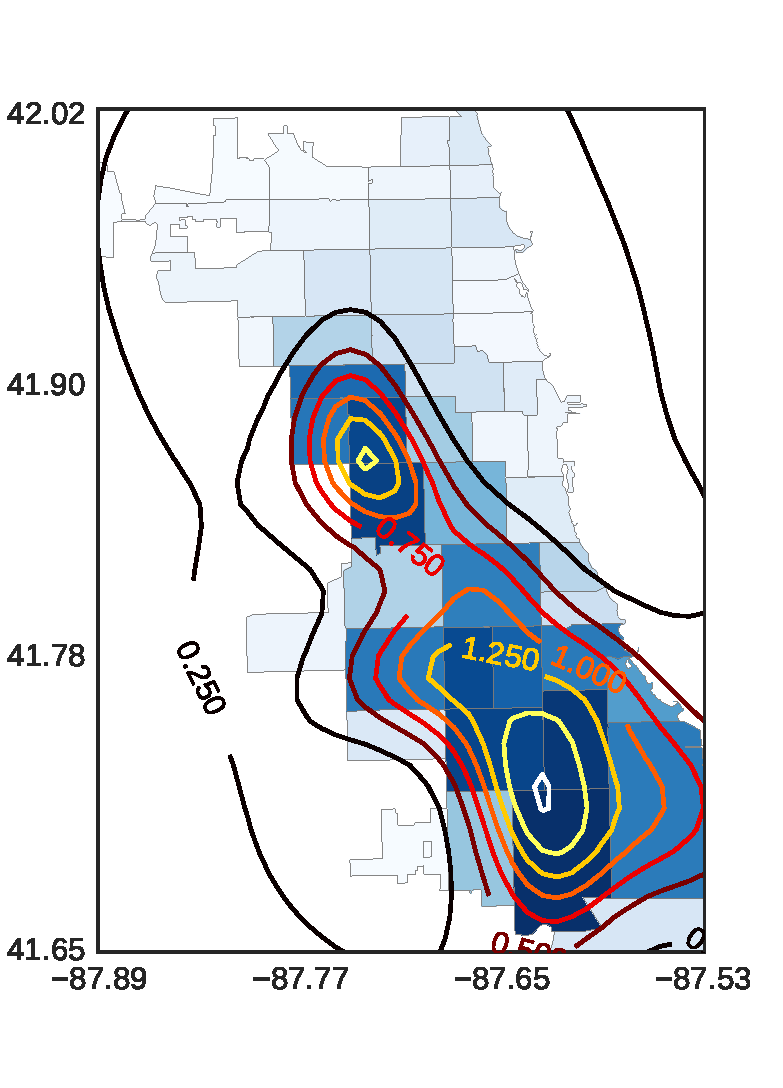
\includegraphics[width=0.33\textwidth,keepaspectratio]{../diagrams/crime_func_f_fast.pdf}
        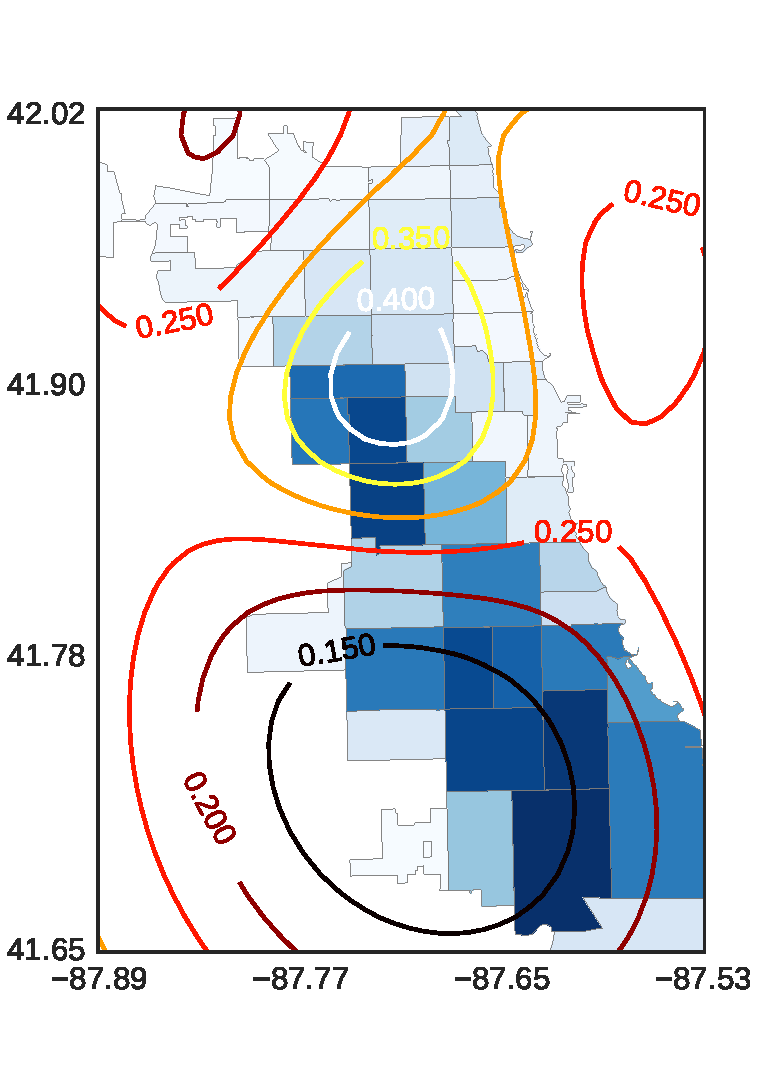
\includegraphics[width=0.33\textwidth,keepaspectratio]{../diagrams/crime_func_g_slow.pdf}\\
        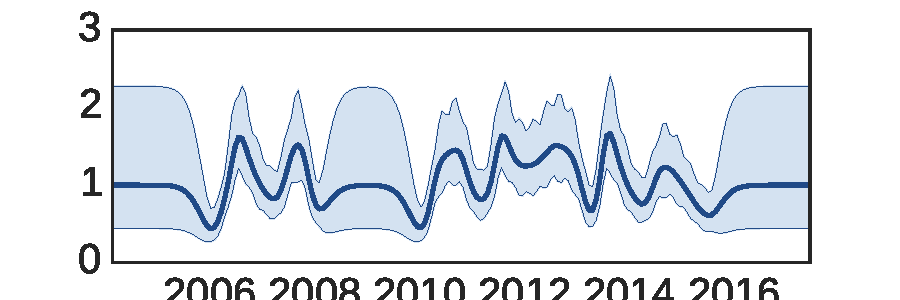
\includegraphics[width=0.33\textwidth,keepaspectratio]{../diagrams/time_f_fig.pdf}
        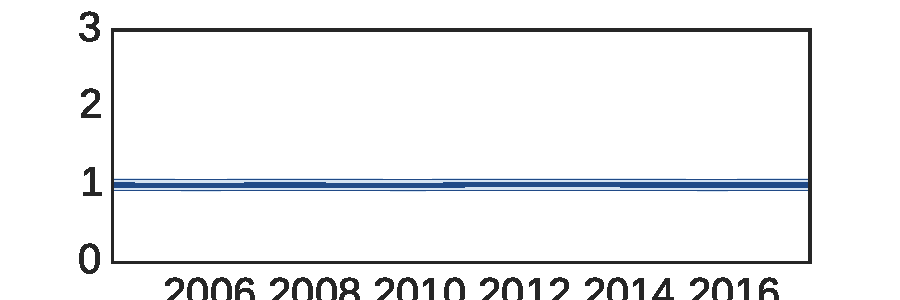
\includegraphics[width=0.33\textwidth,keepaspectratio]{../diagrams/time_g_fig.pdf}\\
    \end{center}
    \begin{itemize}
        %\item Rate parameter of Poisson as sum of spatial GP and temporal GP.
        \item $\Lambda(\xV, \mathbf{t}) = \lambda_1(\xV)\mu_1(\mathbf{t}) + \lambda_2(\xV)\mu_2(\mathbf{t})$
    \end{itemize}
}
%Homicide rate maps for Chicago. The short length scale spatial process, $\lambda_1(x)$ (above-left) is multiplied in the model by a temporal process, $\mu_1(t)$ (below-left) which fluctuates with passing seasons. Contours of spatial process are plotted as deaths per month per zip code area. Error bars on temporal processes are at 5th and 95th percentile. The longer length scale spatial process, $\lambda_2(x)$ (above-right) has been modeled with little to no fluctuation temporally $\mu_2(t)$ (below-right)


\frame[allowframebreaks]{%
    \frametitle{References}
    {\small
    \bibliography{lawrence,other,zbooks,../library}
    %\bibliography{lawrence.bib,other.bib,zbooks.bib,../library.bib}
    }
}

\end{document}
